% LaTeX source for textbook ``How to think like a computer scientist''
% Copyright (C) 1999  Allen B. Downey
% Copyright (C) 2009  Thomas Scheffler


\documentclass[a4paper]{book}
\usepackage[ngerman,english]{babel}
\usepackage[latin1]{inputenc}
\usepackage[T1]{fontenc}
\usepackage{lmodern}
\usepackage{epsfig}
\usepackage{imakeidx}
\usepackage{url}
\usepackage{fancyhdr}
\usepackage{multicol}
\usepackage[hidelinks]{hyperref}
\usepackage{longtable}
\usepackage{ifthen}
\usepackage{boxedminipage}
\usepackage{todonotes}
% conditional compilation of the document for different languages


%\newboolean{German}
%\setboolean{German}{false}

% the exercise environment

\newcounter{exercisenum}                                                  
     
% by default, the exercise number includes the chapter number             
% this way, an exercise label is a complete, unique exercise id           
     
\renewcommand{\theexercisenum}{{\thechapter}.\arabic{exercisenum}}  

% Standard font size for exercise/problem text                            

\newenvironment{exercisesize}{\begin{small}}{\end{small}}                 

\newcommand{\exerciseheader}[2]{                                          
     
  \begin{exercisesize}                                                    
     
  % Use alphabetic chars for subparts of exercises,                            
  % and roman numerals for subparts of them.
     
  \def\theenumi{\alph{enumi}}                                             
  \def\labelenumi{\theenumi.}                                             
  \def\theenumii{\roman{enumii}}                                          
  \def\labelenumii{\theenumii.}                                           
  {\bf Exercise {#1}{#2}}\hspace{0.1in}                 
}                                                                         

\newcommand{\startexercise}[1]{%
  \refstepcounter{exercisenum}                                            
  \exerciseheader{\theexercisenum}{#1}                                    
}                                                                         

\newcommand{\stopexercise}{%                                                   
  {\hfill}                                                               
  \end{exercisesize}      
}                                                         
     
\newcommand{\normaldif}{}                                                 
     
\newcommand{\bigdif}{\dag{}}                                              
     
\newcommand{\verybigdif}{\ddag{}}             

\newenvironment{exercise}{\startexercise{\normaldif{}}}{\stopexercise}    
     
\newenvironment{hardexercise}{\startexercise{\bigdif{}}}{\stopexercise}   
     
%% end of the exercise environment


%%------------------------------------------------------------
% formatting commands

\sloppy
\setlength{\topmargin}{0.125in}
\setlength{\oddsidemargin}{0.875in}
\setlength{\evensidemargin}{0.875in}

\setlength{\headsep}{3ex}
\setlength{\textheight}{8in}

\setlength{\parindent}{0.0in}
\setlength{\parskip}{1.7ex plus 0.5ex minus 0.5ex}
\renewcommand{\baselinestretch}{1.02}

% see LaTeX Companion page 62
\setlength{\topsep}{-0.0\parskip}
\setlength{\partopsep}{-0.5\parskip}
\setlength{\itemindent}{0.0in}
\setlength{\listparindent}{0.0in}

% see LaTeX Companion page 26
% these are copied from /usr/local/teTeX/share/texmf/tex/latex/base/book.cls
% all I changed is afterskip

\makeatletter
\renewcommand{\section}{\@startsection 
    {section} {1} {0mm}%
    {-3.5ex \@plus -1ex \@minus -.2ex}%
    {0.7ex \@plus.2ex}%
    {\normalfont\Large\bfseries}}
\renewcommand\subsection{\@startsection {subsection}{2}{0mm}%
    {-3.25ex\@plus -1ex \@minus -.2ex}%
    {0.3ex \@plus .2ex}%
    {\normalfont\large\bfseries}}
\renewcommand\subsubsection{\@startsection {subsubsection}{3}{0mm}%
    {-3.25ex\@plus -1ex \@minus -.2ex}%
    {0.3ex \@plus .2ex}%
    {\normalfont\normalsize\bfseries}}

\makeatother

\newcommand{\beforeverb}{\vspace{0.6\parskip}}
\newcommand{\afterverb}{\vspace{0.6\parskip}}

\newcommand{\adjustpage}[1]{\enlargethispage{#1\baselineskip}}
\newcommand{\clearemptydoublepage}{\newpage{\pagestyle{empty}\cleardoublepage}}
\newcommand{\blankpage}{\pagestyle{empty}\vspace*{1in}\newpage}

\newcommand{\beforefig}{\vspace{1.3\parskip}}
\newcommand{\afterfig}{\vspace{-0.2\parskip}}
\newcommand{\myfig}[1]{
    \beforefig
    \centerline{\epsfig{#1,scale=0.8}}
    \afterfig
}

\newcommand{\beforechapter}{
%    \clearemptydoublepage 
    \cleardoublepage 
    \setcounter{exercisenum}{0}
}

\pagestyle{fancyplain}

\renewcommand{\chaptermark}[1]{\markboth{#1}{}}
\renewcommand{\sectionmark}[1]{\markright{\thesection\ #1}{}}

\lhead[\fancyplain{}{\bfseries\thepage}]%
      {\fancyplain{}{\bfseries\rightmark}}
\rhead[\fancyplain{}{\bfseries\leftmark}]%
      {\fancyplain{}{\bfseries\thepage}}
\cfoot{}

% turn off the rule under the header
%\setlength{\headrulewidth}{0pt}

% the following is a brute-force way to prevent the headers
% from getting transformed into all-caps
\renewcommand\MakeUppercase{}


\sloppy
\setlength{\topmargin}{0.75in}
\setlength{\headsep}{0.5in}
\setlength{\oddsidemargin}{1.0in}
\setlength{\evensidemargin}{.95in}
\makeindex


%%-----------------------------------------------------------
% beginning of the document

\begin{document}

\thispagestyle{empty}

\begin{flushright}
\vspace*{2.5in}

{\huge How to Think Like a Computer Scientist}

\vspace{0.25in}

{\LARGE C Version}

\vspace{1in}

{\Large Michael Penta}

{based on previous work by Allen B. Downey and Thomas Scheffler}

\vspace{1in}

{\Large Version 1.11}

{\small February 1, 2023}
\vfill

\end{flushright}



Copyright (C) 1999  Allen B. Downey\\
Copyright (C) 2009  Thomas Scheffler\\
Copyright (C) 2023 Michael Penta\\

\vspace{0.25in}

Permission is granted to copy, distribute, transmit and adapt this
work under the Creative Commons Attribution-NonCommercial-ShareAlike 4.0
International License: \url{https://creativecommons.org/licenses/by-nc/4.0/}.

If you are interested in distributing a commercial version of this
work, please contact the author(s).

The \LaTeX\ source and code for this book is available from: \\
\url{https://github.com/tscheffl/ThinkC}

\frontmatter
\tableofcontents


\mainmatter
% LaTeX source for textbook ``How to think like a computer scientist''
% Copyright (C) 1999  Allen B. Downey
% Copyright (C) 2009  Thomas Scheffler

\chapter{The way of the program}
\label{chap01}

The goal of this book, and this class, is to teach you to think like a
computer scientist.  I like the way computer scientists think because
they combine some of the best features of Mathematics, Engineering,
and Natural Science.  Like mathematicians, computer scientists use formal
languages to denote ideas (specifically computations).  Like
engineers, they design things, assembling components into systems and
evaluating tradeoffs among alternatives.  Like scientists,
they observe the behavior of complex systems, form hypotheses, and test
predictions.

The single most important skill for a computer scientist is {\bf
problem-solving}.  By that I mean the ability to formulate problems,
think creatively about solutions, and express a solution clearly and
accurately.  As it turns out, the process of learning to program is an
excellent opportunity to practice problem-solving skills.  That's why
this chapter is called ``The way of the program.''

On one level, you will be learning to program, which is a useful
skill by itself.  On another level you will use programming
as a means to an end.  As we go along, that end will
become clearer.

\section{What is a programming language?}
\index{programming language}
\index{language!programming}

The programming language you will be learning is C, which was developed
in the early 1970s by Dennis M. Ritchie at the Bell Laboratories.  C is
an example of a {\bf high-level language}; other high-level languages
you might have heard of are Pascal, C++ and Java.

As you might infer from the name ``high-level language,'' there are
also {\bf low-level languages}, sometimes referred to as machine
language or assembly language.  Loosely-speaking, computers can only
execute programs written in low-level languages.  Thus, programs
written in a high-level language have to be translated before they can
run.  This translation takes some time, which is a small disadvantage
of high-level languages.

\index{portable}
\index{high-level language}
\index{low-level language}
\index{language!high-level}
\index{language!low-level}

But the advantages are enormous.  First,
it is {\em much} easier to program in a high-level language;
by ``easier'' I mean that the program takes less time to write,
it's shorter and easier to read, and it's more likely to be
correct.  Secondly, high-level languages are {\bf portable},
meaning that they can run on different kinds of computers with
few or no modifications.  Low-level programs can only run
on one kind of computer, and have to be rewritten to run on
another.

Due to these advantages, almost all programs are written in
high-level languages.  Low-level languages are only used for
a few special applications.

\index{compile}
\index{interpret}

There are two ways to translate a program;
{\bf interpreting} or {\bf compiling}.  An interpreter
is a program that reads a high-level program
and does what it says.  In effect, it translates
the program line-by-line, alternately reading lines and
carrying out commands.

\vskip 0.7em
\centerline{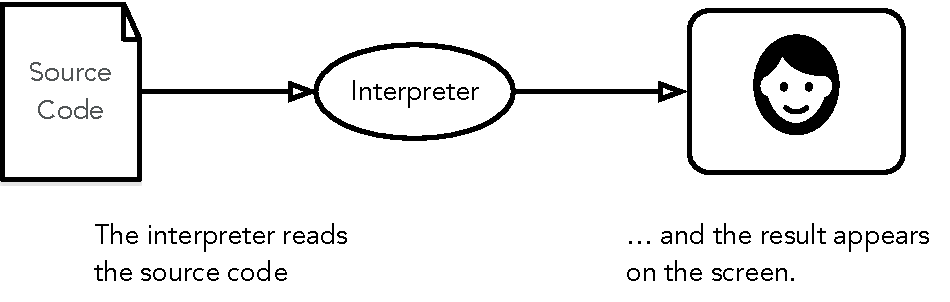
\includegraphics[height=3cm]{figs/Interpreter}}

A compiler is a program that reads a high-level program and
translates it all at once, before executing any of the commands.
Often you compile the program as a separate step, and then
execute the compiled code later.  In this case, the high-level
program is called the {\bf source code}, and the translated
program is called the {\bf object code} or the {\bf executable}.

As an example, suppose you write a program in C.  You might
use a text editor to write the program (a text editor is
a simple word processor).  When the program is finished, you
might save it in a file named {\tt program.c}, where ``program''
is an arbitrary name you make up, and the suffix {\tt .c} is
a convention that indicates that the file contains C source
code.

Then, depending on what your programming environment is like,
you might leave the text editor and run the compiler.  The
compiler would read your source code, translate it, and create
a new file named {\tt program.o} to contain the object code,
or {\tt program.exe} to contain the executable. 

\vskip 0.7em
\centerline{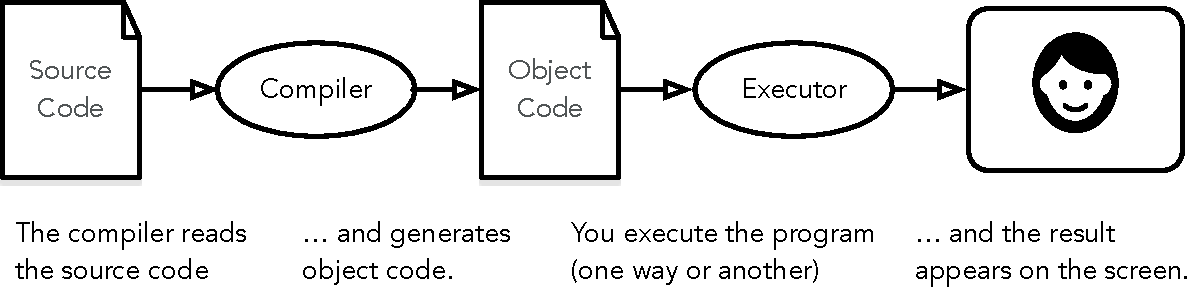
\includegraphics[height=3cm]{figs/Compiler}}


The next step is to run the program, which requires some kind of executor. 
The role of the executor is to load the program (copy it from disk into memory) 
and make the computer start executing the program. 


Although this process may seem complicated, in most programming
environments (sometimes called development environments), these steps
are automated for you.  Usually you will only have to write a program
and press a button or type a single command to compile and run it.  On
the other hand, it is useful to know what the steps are that are
happening in the background, so that if something goes wrong you can
figure out what it is.

% Leftover: when is compilation better than interpretation?

\section{What is a program?}

A program is a sequence of instructions that
specifies how to perform a computation.  The computation might be
something mathematical, like solving a system of equations or finding
the roots of a polynomial, but it can also be a symbolic computation,
like searching and replacing text in a document or (strangely enough)
compiling a program.

\index{statement}

The instructions, which we will call {\bf statements}, look different
in different programming languages, but there are a few basic
operations most languages can perform:

\begin{description}

\item[input:] Get data from the keyboard, or a file, or some
other device.

\item[output:] Display data on the screen or send data to a
file or other device.

\item[math:] Perform basic mathematical operations like addition and
multiplication.

\item[testing:] Check for certain conditions and execute the
appropriate sequence of statements.

\item[repetition:] Perform some action repeatedly, usually with
some variation.

\end{description}

That's pretty much all there is to it.
Every program you've ever used, no matter how complicated, is
made up of statements that perform these operations.  Thus,
one way to describe programming is the process of breaking a
large, complex task up into smaller and smaller subtasks
until eventually the subtasks are simple enough to be performed
with one of these basic operations.

\section{What is debugging?}
\index{debugging}
\index{bug}

Programming is a complex process, and since it is done by
human beings, it often leads to errors.  For whimsical reasons,
programming errors are called {\bf bugs} and the process
of tracking them down and correcting them is called
{\bf debugging}.

There are a few different kinds of errors that can occur
in a program, and it is useful to distinguish between them
in order to track them down more quickly.

\subsection{Compile-time errors}
\index{compile-time error}
\index{error!compile-time}

The compiler can only translate a program if the program is
syntactically correct; otherwise, the compilation fails and
you will not be able to run your program.  {\bf Syntax}
refers to the structure of your program and the rules about
that structure.

\index{syntax}

For example, in English, a sentence must begin with a capital
letter and end with a period.  this sentence contains a syntax
error.  So does this one

For most readers, a few syntax errors are not a significant
problem, which is why we can read the poetry of E.~E.~Cummings
without spewing error messages.

Compilers are not so forgiving.  If there is a single syntax
error anywhere in your program, the compiler will print an
error message and quit, and you will not be able to run
your program.

To make matters worse, there are more syntax rules in C
than there are in English, and the error messages you get from
the compiler are often not very helpful.  During the first
few weeks of your programming career, you will probably
spend a lot of time tracking down syntax errors.  As you
gain experience, though, you will make fewer errors and find
them faster.

\subsection{Run-time errors}
\label{run-time}
\index{run-time error}
\index{error!run-time}
%\index{exception}
\index{safe language}
\index{language!safe}

The second type of error is a run-time error, so-called because
the error does not appear until you run the program.  

C is not a {\bf safe} language, such as Java, where
run-time errors are rare. Programming in C allows you to get very close to the actual
computing hardware. Most run-time errors C occur because the
language provides no protection against the accessing or
overwriting of data in memory.

For the simple sorts of programs we will be writing for the next few weeks, 
run-time errors are rare, so it might be a little while before you encounter one.


\subsection{Logic errors and semantics}
\index{semantics}
\index{logic error}
\index{error!logic}

The third type of error is the {\bf logical} or {\bf semantic}
error.  If there is a logical error in your program, it will
compile and run successfully, in the sense that the computer
will not generate any error messages, but it will not do the
right thing.  It will do something else.  Specifically, it will
do what you told it to do.

The problem is that the program you wrote is not the program
you wanted to write.  The meaning of the program (its semantics)
is wrong.  Identifying logical errors can be tricky, since
it requires you to work backwards by looking at the output
of the program and trying to figure out what it is doing.

\subsection{Experimental debugging}

One of the most important skills you will acquire in this
class is debugging.  Although it can be frustrating, debugging
is one of the most intellectually rich, challenging, and
interesting parts of programming.

In some ways debugging is like detective work.  You are
confronted with clues and you have to infer the processes
and events that lead to the results you see.

Debugging is also like an experimental science.  Once you have an idea
what is going wrong, you modify your program and try again.  If your
hypothesis was correct, then you can predict the result of the
modification, and you take a step closer to a working program.  If
your hypothesis was wrong, you have to come up with a new one.  As
Sherlock Holmes pointed out, ``When you have eliminated the
impossible, whatever remains, however improbable, must be the truth.''
(from A. Conan Doyle's {\em The Sign of Four}).

\index{Holmes, Sherlock}
\index{Doyle, Arthur Conan}

For some people, programming and debugging are the
same thing.  That is, programming is the process of gradually
debugging a program until it does what you want.  The idea
is that you should always start with a working program that
does {\em something}, and make small modifications, debugging
them as you go, so that you always have a working program.

For example, Linux is an operating system that contains thousands of
lines of code, but it started out as a simple program Linus Torvalds
used to explore the Intel 80386 chip.  According to Larry Greenfield,
``One of Linus's earlier projects was a program that would switch
between printing AAAA and BBBB.  This later evolved to Linux''
(from {\em The Linux Users' Guide} Beta Version 1).

\index{Linux}

In later chapters I will make more suggestions about debugging
and other programming practices.

\section{Formal and natural languages}
\index{formal language}
\index{natural language}
\index{language!formal}
\index{language!natural}

{\bf Natural languages} are the languages that people speak,
like English, Spanish, and French.  They were not designed
by people (although people try to impose some order on them);
they evolved naturally.

{\bf Formal languages} are languages that are designed by people for
specific applications.  For example, the notation that mathematicians
use is a formal language that is particularly good at denoting
relationships among numbers and symbols.  Chemists use a formal
language to represent the chemical structure of molecules.  And
most importantly:

\begin{quote}
{\bf Programming languages are formal languages that have been
designed to express computations.}
\end{quote}

As I mentioned before, formal languages tend to have strict rules
about syntax.  For example, $3+3=6$ is a syntactically correct
mathematical statement, but $3=+6\$$ is not.  Also, $H_2O$ is a
syntactically correct chemical name, but $_2Zz$ is not.

Syntax rules come in two flavors, pertaining to tokens and structure.
Tokens are the basic elements of the language, like words and numbers
and chemical elements.  One of the problems with {\tt 3=+6\$} is that
{\tt \$} is not a legal token in mathematics (at least as far as I
know).  Similarly, $_2Zz$ is not legal because there is no element with
the abbreviation $Zz$.

The second type of syntax rule pertains to the structure of a
statement; that is, the way the tokens are arranged.  The statement
{\tt 3=+6\$} is structurally illegal, because you can't have a plus
sign immediately after an equals sign.  Similarly, molecular formulas
have to have subscripts after the element name, not before.

When you read a sentence in English or a statement in a formal
language, you have to figure out what the structure of the sentence is
(although in a natural language you do this unconsciously).  This
process is called {\bf parsing}.

\index{parse}

For example, when you hear the sentence, ``The other shoe fell,'' you
understand that ``the other shoe'' is the subject and ``fell'' is the
verb.  Once you have parsed a sentence, you can figure out what it
means, that is, the semantics of the sentence.  Assuming that you know
what a shoe is, and what it means to fall, you will understand the
general implication of this sentence.

Although formal and natural languages have many features in
common---tokens, structure, syntax and semantics---there are many
differences.

\index{ambiguity}
\index{redundancy}
\index{literalness}

\begin{description}

\item[ambiguity:] Natural languages are full of ambiguity, which
people deal with by using contextual clues and other information.
Formal languages are designed to be nearly or completely unambiguous,
which means that any statement has exactly one meaning,
regardless of context.

\item[redundancy:] In order to make up for ambiguity and reduce
misunderstandings, natural languages employ lots of
redundancy.  As a result, they are often verbose.  Formal languages
are less redundant and more concise.

\item[literalness:] Natural languages are full of idiom and
metaphor.  If I say, ``The other shoe fell,'' there is probably
no shoe and nothing falling.  Formal languages mean
exactly what they say.

\end{description}

People who grow up speaking a natural language (everyone) often have a
hard time adjusting to formal languages.  In some ways the difference
between formal and natural language is like the difference between
poetry and prose, but more so:

\index{poetry}
\index{prose}

\begin{description}

\item[Poetry:] Words are used for their sounds as well as for
their meaning, and the whole poem together creates an effect or
emotional response.  Ambiguity is not only common but often
deliberate.

\item[Prose:] The literal meaning of words is more important
and the structure contributes more meaning.  Prose is more amenable to
analysis than poetry, but still often ambiguous.

\item[Programs:] The meaning of a computer program is unambiguous
and literal, and can be understood entirely by analysis of the
tokens and structure.

\end{description}

Here are some suggestions for reading programs (and other formal
languages).  First, remember that formal languages are much more dense
than natural languages, so it takes longer to read them.  Also, the
structure is very important, so it is usually not a good idea to read
from top to bottom, left to right.  Instead, learn to parse the
program in your head, identifying the tokens and interpreting the
structure.  Finally, remember that the details matter.  Little things
like spelling errors and bad punctuation, which you can get away
with in natural languages, can make a big difference in a formal
language.

\section{The first program}
\label{hello}
\index{hello world}

Traditionally the first program people write in a new language
is called ``Hello, World.'' because all it does is display the
words ``Hello, World.''  In C, this program looks like this:

\begin{verbatim}
  #include <stdio.h>
  #include <stdlib.h>

  /* main: generate some simple output */

  int main(void)
  {
        printf("Hello, World.\n");
        return(EXIT_SUCCESS);
  }

\end{verbatim}
%
Some people judge the quality of a programming language by
the simplicity of the ``Hello, World.'' program.  By this
standard, C does reasonably well.  Even so, this simple program 
contains several features that are hard to explain 
to beginning programmers. For now, we will ignore some of them, 
like the first two lines.

\index{comment}
\index{statement!comment}

The third line begins with {\tt /*} and ends with  {\tt */}, which indicates
that it is a {\bf comment}.  A comment is a bit of
English text that you can put in the middle of a program,
usually to explain what the program does.  When the compiler
sees a {\tt /*}, it ignores everything from there until it finds the corresponding
 {\tt */}.

In the forth line, you notice the word {\tt main}.  {\tt main} is a
special name that indicates the place in the program where execution
begins.  When the program runs, it starts by executing the first
{\bf statement} in {\tt main()} and it continues, in order, until it gets
to the last statement, and then it quits.


\index{printf()}
\index{statement!printf}	

There is no limit to the number of statements that can be in 
{\tt main()}, but the example contains only two. 
The first  is an {\bf output} statement, 
meaning that it displays or prints a message on the screen.
The second statement tells the operating system that our program
executed successfully.  

The statement that prints things on the screen is
{\tt printf()}, and the characters between the quotation marks
will get printed. Notice the {\tt \textbackslash n} after the 
last character. This is a special character called \emph{newline} that is appended at the end 
of a line of text  and causes the cursor to move to the next line of the display. 
The next time you output something, the new text appears on the next line.
At the end of the statement
there is a semicolon ({\tt ;}), which is required at the end
of every statement.

There are a few other things you should notice about the syntax
of this program.  First, C uses curly-brackets (\{ and
\}) to group things together. 
In this case, the output statement
is enclosed in curly-brackets, indicating that it is {\em inside} the
definition of {\tt main()}.  Also, notice that the statement is
indented, which helps to show visually which lines are inside the
definition.

At this point it would be a good idea to sit down in front of
a computer and compile and run this program.  The details of how
to do that depend on your programming environment, this book 
assumes that you know how to do it.

As I mentioned, the C compiler is very pedantic with syntax.
If you make any errors when you type in the program, chances
are that it will not compile successfully.  For example, if
you misspell {\tt stdio.h}, you might get an error message like
the following:

\begin{verbatim}
   hello_world.c:1:19: error: sdtio.h: No such file or directory
\end{verbatim}
%
There is a lot of information on this line, but it is presented
in a dense format that is not easy to interpret.  A more friendly
compiler might say something like:

\begin{quote}
``On line 1 of the source code file named hello\_world.c, you tried to
include a header file named sdtio.h.  I didn't find anything
with that name, but I did find something named stdio.h.  Is
that what you meant, by any chance?''
\end{quote}

Unfortunately, few compilers are so accommodating.  The compiler
is not really very smart, and in most cases the error message
you get will be only a hint about what is wrong.  It will take
some time for you to learn to interpret different compiler messages.

Nevertheless, the compiler can be a useful tool for learning the
syntax rules of a language.  Starting with a working program
(like hello\_world.c), modify it in various ways and see what happens.
If you get an error message, try to remember what the message says
and what caused it, so if you see it again in the future you
will know what it means.





\section{Glossary}

\begin{description}

\item[problem-solving:]  The process of formulating a problem, finding
a solution, and expressing the solution.

\item[high-level language:]  A programming language like C that
is designed to be easy for humans to read and write.

\item[low-level language:]  A programming language that is designed
to be easy for a computer to execute.  Also called ``machine
language'' or ``assembly language.''

\item[formal language:]  Any of the languages people have designed
for specific purposes, like representing mathematical ideas or
computer programs.  All programming languages are formal languages.

\item[natural language:]  Any of the languages people speak that
have evolved naturally.

\item[portability:]  A property of a program that can run on more
than one kind of computer.

\item[interpret:]  To execute a program in a high-level language
by translating it one line at a time.

\item[compile:]  To translate a program in a high-level language
into a low-level language, all at once, in preparation for later
execution.

\item[source code:]  A program in a high-level language, before
being compiled.

\item[object code:]  The output of the compiler, after translating
the program.

\item[executable:]  Another name for object code that is ready
to be executed.

\item[statement:] A part of a program that specifies an action
that will be performed when the program runs.  A print statement
causes output to be displayed on the screen.

\item[comment:] A part of a program that contains information
about the program, but that has no effect when the program runs.

\item[algorithm:]  A general process for solving a category of
problems.

\item[bug:]  An error in a program.

\item[syntax:]  The structure of a program.

\item[semantics:]  The meaning of a program.

\item[parse:]  To examine a program and analyze the syntactic structure.

\item[syntax error:]  An error in a program that makes it impossible
to parse (and therefore impossible to compile).

%\item[exception:]  An error in a program that makes it fail at
%run-time.  Also called a run-time error.

\item[logical error:]  An error in a program that makes it do something
other than what the programmer intended.

\item[debugging:]  The process of finding and removing any of
the three kinds of errors.

\index{problem-solving}
\index{high-level language}
\index{low-level language}
\index{formal language}
\index{natural language}
\index{interpret}
\index{compile}
\index{syntax}
\index{semantics}
\index{parse}
%\index{exception}
\index{error}
\index{debugging}
\index{statement}
\index{comment}

\end{description}

\section{Exercises}

% LaTeX source for textbook ``How to think like a computer scientist''
% Copyright (C) 1999  Allen B. Downey
% Copyright (C) 2009  Thomas Scheffler

\begin{exercise}

Computer scientists have the annoying habit of using common
English words to mean something different from their common
English meaning.  For example, in English, a statement and
a comment are pretty much the same thing, but when we are
talking about a program, they are very different.

The glossary at the end of each chapter is intended to highlight
words and phrases that have special meanings in computer science.
When you see familiar words, don't assume that you know what 
they mean!

\begin{enumerate}

\item In computer jargon, what's the difference between a statement
and a comment?

\item What does it mean to say that a program is portable?

\item What is an executable?

\end{enumerate}

\end{exercise}

\begin{exercise}

Before you do anything else, find out how to compile and run a C
program in your environment.  Some environments provide sample programs
similar to the example in Section~\ref{hello}.

\begin{enumerate}

\item Type in the ``Hello World'' program, then compile and run it.

\item Add a second print statement that prints a second message after
the ``Hello World.''.  Something witty like, ``How are you?''
Compile and run the program again.

\item Add a comment line to the program (anywhere) and recompile
it.  Run the program again.  The new comment should not affect the
execution of the program.

\end{enumerate}

This exercise may seem trivial, but it is the starting place for many
of the programs we will work with.  In order to debug with confidence,
you have to have confidence in your programming environment.  In some
environments, it is easy to lose track of which program is executing,
and you might find yourself trying to debug one program while you are
accidentally executing another.  Adding (and changing) print statements
is a simple way to establish the connection between the program you
are looking at and the output when the program runs.

\end{exercise}


\begin{exercise}

It is a good idea to commit as many errors as you can think of,
so that you see what error messages the compiler produces.
Sometimes the compiler will tell you exactly what is wrong, and all
you have to do is fix it.  Sometimes, though, the compiler will produce
wildly misleading messages.  You will develop a sense for when you can
trust the compiler and when you have to figure things out yourself.

\begin {enumerate}

\item Remove the closing curly-bracket (\}).

\item Remove the opening curly-bracket (\{).

\item Remove the {\tt int} before {\tt main}.

\item Instead of {\tt main}, write {\tt mian}.

\item Remove the closing {\tt */} from a comment.

\item Replace {\tt printf} with {\tt pintf}.

% Example of a logical error:
%
%\item Replace {\tt printf} with {\tt print}.  This one is
%tricky because it is a logical error, not a syntax error.
%The statement {\tt System.out.print} is legal, but it may or may
%not do what you expect.

\item Delete one of the parentheses:  {\tt (} or  {\tt )}.  Add an extra one.

\item Delete the semicolon after the {\tt return} statement.

\end {enumerate}
\end{exercise}


% LaTeX source for textbook ``How to think like a computer scientist''
% Copyright (C) 1999  Allen B. Downey
% Copyright (C) 2009  Thomas Scheffler

\setcounter{chapter}{1}
\chapter{Variables and types}

\section{More output}
\index{output}
\index{statement!output}

As I mentioned in the last chapter, you can put as many statements as
you want in {\tt main()}.  For example, to output more than one line:

\begin{verbatim}

  #include <stdio.h>
  #include <stdlib.h>

  /* main: generate some simple output */

  int main (void)
  {
        printf ("Hello World.\n");		    /* output one line */
        printf ("How are you?\n");		    /* output another line */       
        return (EXIT_SUCCESS);
  }

\end{verbatim}
%
As you can see, it is legal to put comments at the
end of a line, as well as on a line by themselves.

\index{String}
\index{type!String}

The phrases that appear in quotation marks are called {\bf strings},
because they are made up of a sequence (string) of letters.  Actually,
strings can contain any combination of letters, numbers, punctuation
marks, and other special characters.

\index{newline}

Often it is useful to display the output from multiple output
statements all on one line.  You can do this by leaving out
the {\tt $\backslash$n} from the first {\tt printf}:

\begin{verbatim}
  int main (void)
  {
        printf ("Goodbye, ");
        printf ("cruel world!\n");	     
        return (EXIT_SUCCESS);
  }
\end{verbatim}
%
In this case the output appears on a single line as
{\tt Goodbye, cruel world!}.  Notice that there is a space
between the word ``Goodbye,'' and the second quotation mark.
This space appears in the output, so it affects the behavior
of the program.

Spaces that appear outside of quotation marks generally do
not affect the behavior of the program.  For example, I
could have written:

\begin{verbatim}
  int main(void)
  {
  printf("Goodbye, ");
  printf("cruel world!\n");	     
  return(EXIT_SUCCESS);
  }
\end{verbatim}
%
This program would compile and run just as well as the original.
The breaks at the ends of lines (newlines) do not affect
the program's behavior either, so I could have written:

\begin{verbatim}
  int main(void){printf("Goodbye, ");printf("cruel world!\n");
  return(EXIT_SUCCESS);}
\end{verbatim}
%
That would work, too, although you have probably noticed that
the program is getting harder and harder to read.  Newlines and
spaces are useful for organizing your program visually, making
it easier to read the program and locate syntax errors.

\section{Values}
\index{value}
\index{type}

Computer programs operate on values stored in 
computer memory.
A value ---like a letter or
a number--- is one of the fundamental things that a program manipulates.  
The only values we have
manipulated so far are the strings we have been outputting, like
{\tt "Hello, world."}.  You (and the compiler) can identify
these string values because they are enclosed in quotation marks.
%constant values

There are different kinds of values, including integers and characters.
It is important for the program to know exactly what kind of value
is manipulated because not all manipulations will make sense on all
values.
We therefore distinguish between different {\bf types} of values.  
%Example 'a' + 'a'

An integer is a whole number like 1 or 17.  You can output
integer values in a similar way as you output strings:

\begin{verbatim}
   printf("%i\n", 17);
\end{verbatim}
%
When we look at the \texttt{printf()} statement more closely, we
notice that the value we are outputting no longer appears
inside the quotes, but behind them separated by comma.
The string is still there, but now contains a {\tt \%i} instead of
any text. 
The {\tt \%i} a placeholder that tells the \texttt{printf()} command
to print an integer value. Several such placeholders exist
for different data types and formatting options of the output.
We will see the next one just now.

A character value is a letter or digit or punctuation mark
enclosed in single quotes, like {\tt 'a'} or {\tt '5'}.
You can output character values in a similar way:

\begin{verbatim}
   printf("%c\n", '}');
\end{verbatim}
%
This example outputs a single closing curly-bracket on a line
by itself. It uses the {\tt \%c} placeholder to signify the output of a character
value.

It is easy to confuse different types of values, like {\tt "5"}, {\tt
'5'} and {\tt 5}, but if you pay attention to the punctuation, it
should be clear that the first is a string, the second is a character
and the third is an integer.  The reason this distinction is important
should become clear soon.

\section {Variables}
\index{variable}
\index{value}

One of the most powerful features of a programming language is the
ability to manipulate values through the use of {\bf variables}.  So far
the values that we have used in our statements where fixed to what 
was written in the statement. Now we will use a variable as a named 
location that stores a value.  

Just as there are different types of values (integer, character,
etc.), there are different types of variables.  When you create a new
variable, you have to declare what type it is.  For example, the
character type in C is called {\tt char}.  The following statement
creates a new variable named {\tt fred} that has type {\tt char}.

\begin{verbatim}
    char fred;
\end{verbatim}
%
This kind of statement is called a {\bf declaration}.

The type of a variable determines what kind of values it can
store.  A {\tt char} variable can contain characters, and it should
come as no surprise that {\tt int} variables can store integers.

Contrary to other programming languages, C does not have a 
dedicated variable type for the storage of string values. We will see in
a later chapter how string values are stored in C. 
%but we
%are going to skip that for now (see Chapter~\ref{strings}).

\index{declaration}
\index{statement!declaration}

To create an integer variable, the syntax is 

\begin{verbatim}
    int bob;
\end{verbatim}
%
where {\tt bob} is the arbitrary name you choose to identify the
variable.  In general, you will want to make up variable names
that indicate what you plan to do with the variable.  For
example, if you saw these variable declarations:

\begin{verbatim}
    char first_letter;
    char last_letter;
    int hour, minute;
\end{verbatim}
%
you could probably make a good guess at what values
would be stored in them.  This example
also demonstrates the syntax for declaring multiple variables
with the same type: {\tt hour} and {\tt minute}
are both integers ({\tt int} type).

ATTENTION: The older C89 standard allows variable declarations
only at the beginning of a block of code. It is therefore necessary
to put variable declarations before any other statements,
even if the variable itself is only needed much later in your program.

\section{Assignment}
\index{assignment}
\index{statement!assignment}

Now that we have created some variables, we would like to
store values in them.  We do that with an {\bf assignment
statement}.

\begin{verbatim}
    first_letter = 'a';   /* give first_letter the value 'a' */
    hour = 11;            /* assign the value 11 to hour */
    minute = 59;          /* set minute to 59 */
\end{verbatim}
%
This example shows three assignments, and the comments show
three different ways people sometimes talk about assignment
statements.  The vocabulary can be confusing here, but the
idea is straightforward:

\begin{itemize}

\item When you declare a variable, you create a named storage location.

\item When you make an assignment to a variable, you give it a value.

\end{itemize}

A common way to represent variables on paper is to draw a box
with the name of the variable on the outside and the value
of the variable on the inside.  This kind of figure is called
a {\bf state diagram} because is shows what state each 
variable is in (you can think of it as the variable's ``state of
mind'').
This diagram shows the effect of the three assignment statements:

%\vspace{0.1in}
%\centerline{\epsfig{figure=figs/assign.eps}}
%\vspace{0.1in}

\setlength{\unitlength}{1mm}
\begin{picture}(20,17)
\put(7,12){\large \texttt{first\_letter}}
\put(46,12){\large \texttt{hour}}
\put(74,12){\large \texttt{minute}}
\put(10,0){\framebox(20,10){{\large \textsf{a}}}}
\put(40,0){\framebox(20,10){{\large \textsf{11}}}}
\put(70,0){\framebox(20,10){{\large \textsf{59}}}}
\end{picture}

When we assign values to variables, we have to make sure that
the assigned value correspondents to the type of the variable.
In C  a variable has to have the same type as the
value you assign.  For example, you cannot store a string in
an {\tt int} variable.  The following statement generates a compiler
warning:

\begin{verbatim}
    int hour;
    hour = "Hello.";       /* WRONG !! */
\end{verbatim}
%
This rule is sometimes a source of confusion, because there are many
ways that you can convert values from one type to another, and C
sometimes converts things automatically.  But for now you should
remember that as a general rule variables and values have the same
type, and we'll talk about special cases later.

Another source of confusion is that some strings {\em look}
like integers, but they are not.  For example,
the string {\tt "123"}, which is made up of the
characters {\tt 1}, {\tt 2} and {\tt 3}, is not
the same thing as the {\em number} {\tt 123}.
This assignment is illegal:

\begin{verbatim}
    minute = "59";         /* WRONG!! */
\end{verbatim}
%
\section{Outputting variables}
\label{output variables}

You can output the value of a variable using the same commands
we used to output simple values.

\begin{verbatim}

    int hour, minute;
    char colon;

    hour = 11;
    minute = 59;
    colon = ':';

    printf ("The current time is ");
    printf ("%i", hour);
    printf ("%c", colon);
    printf ("%i", minute);
    printf ("\n"); 
  
\end{verbatim}
%
This program creates two integer variables named {\tt hour} and {\tt
minute}, and a character variable named {\tt colon}.  It assigns
appropriate values to each of the variables and then uses a series
of output statements to generate the following:

\begin{verbatim}
    The current time is 11:59
\end{verbatim}

When we talk about ``outputting a variable,'' we mean outputting the
{\em value} of the variable.  The name of a variable only has significance for
the programmer. The compiled program no longer contains a human readable
reference to the variable name in your program. 

The \texttt{ printf()} command is capable of outputting several variables
in a single statement. To do this, we need to put placeholders
in the so called \emph{format string}, that indicate the position where the variable value will
be put. The variables will be inserted in the order of their appearance in 
the statement. It is important to observe the right order and type for the variables.

By using a single output statement, we can make the previous program more
concise:

\begin{verbatim}
    
    int hour, minute;
    char colon;

    hour = 11;
    minute = 59;
    colon = ':';

    printf ("The current time is %i%c%i\n", hour, colon, minute);
    
\end{verbatim}
%
On one line, this program outputs a string, two integers and a character.  Very impressive!

\section{Keywords}
\index{keyword}

A few sections ago, I said that you can make up any name you
want for your variables, but that's not quite true.  There
are certain words that are reserved in C because they are
used by the compiler to parse the structure of your program,
and if you use them as variable names, it will get confused.
These words, called {\bf keywords}, include {\tt int},
{\tt char}, {\tt void} and many more.

\vskip 1em

\setlength{\fboxsep}{6pt} 
\begin{center}
\begin{boxedminipage}[c]{.9\linewidth}
\begin{center}
\begin{multicols}{5}[\underline{Reserved keywords in the C language}]
\begin{verbatim}
auto 
break 
case 
char 
const 
continue 
default 
do 
double 
else 
enum 
extern 
float 
for 
goto 
if 
inline 
int 
long 
register 
restrict 
return 
short 
signed 
sizeof 
static 
struct 
switch 
typedef 
union 
unsigned 
void 
volatile 
while 
_Bool 
_Complex 
_Imaginary 
\end{verbatim}
\end{multicols}
\end{center}
\end{boxedminipage}
\end{center}

\vskip 1em
The complete list of keywords is included in the C Standard, which
is the official language definition adopted by the the International
Organization for Standardization (ISO) on September 1, 1998.  

%You can download a copy electronically from
%
%\begin{verbatim}
%    http://www.ansi.org/
%\end{verbatim}
%
Rather than memorize the list, I would suggest that you
take advantage of a feature provided in many development
environments: code highlighting.  As you type, different
parts of your program should appear in different colors.  For
example, keywords might be blue, strings red, and other code
black.  If you type a variable name and it turns blue, watch
out!  You might get some strange behavior from the compiler.

\section{Operators}
\label{operators}
\index{operator}


{\bf Operators} are special symbols that are used to represent
simple computations like addition and multiplication.  Most
of the operators in C do exactly what you would expect them
to do, because they are common mathematical symbols.  For
example, the operator for adding two integers is {\tt +}.

The following are all legal C expressions whose meaning is
more or less obvious:

\begin{verbatim}
    1+1        hour-1       hour*60+minute     minute/60
\end{verbatim}
%
{\bf Expressions} can contain both variables
names and values.  In each case the name of the variable is
replaced with its value before the computation is performed.

\index{expression}

Addition, subtraction and multiplication all do what you
expect, but you might be surprised by division.  For example,
the following program:

\begin{verbatim}

  int hour, minute;
  hour = 11;
  minute = 59;
  printf ("Number of minutes since midnight: %i\n", hour*60 + minute);
  printf ("Fraction of the hour that has passed: %i\n", minute/60);

\end{verbatim}
%
would generate the following output:

\begin{verbatim}
    Number of minutes since midnight: 719
    Fraction of the hour that has passed: 0
\end{verbatim}
%
The first line is what we expected, but the second line is
odd.  The value of the variable {\tt minute} is 59, and
59 divided by 60 is 0.98333, not 0.  The reason for the
discrepancy is that C is performing {\bf integer division}.

\index{type!int}
\index{integer division}
\index{arithmetic!integer}
\index{division!integer}
\index{operand}

When both of the {\bf operands} are integers (operands are the things
operators operate on), the result must also be an integer,
and by definition integer division always rounds {\em down},
even in cases like this where the next integer is so close.

A possible alternative in this case is to calculate a percentage
rather than a fraction:

\begin{verbatim}
    printf ("Percentage of the hour that has passed: ");
    printf ("%i\n", minute*100/60);
\end{verbatim}
%
The result is:

\begin{verbatim}
    Percentage of the hour that has passed: 98
\end{verbatim}
%
Again the result is rounded down, but at least now the answer
is approximately correct.  In order to get an even more accurate
answer, we could use a different type of variable, called
floating-point, that is capable of storing fractional values.
We'll get to that in the next chapter.

\section{Order of operations}
\index{precedence}
\index{order of operations}

When more than one operator appears in an expression the order
of evaluation depends on the rules of {\bf precedence}.  A
complete explanation of precedence can get complicated, but
just to get you started:

\begin{itemize}

\item Multiplication and division happen before
addition and subtraction.  So {\tt 2*3-1} yields 5, not 4, and {\tt
2/3-1} yields -1, not 1.
%(remember that in integer division {\tt 2/3} is 0).

\item If the operators have the same precedence they are evaluated
from left to right.  So in the expression {\tt minute*100/60},
the multiplication happens first, yielding {\tt 5900/60}, which
in turn yields {\tt 98}.  If the operations had gone from right
to left, the result would be {\tt 59*1} which is {\tt 59}, which
is wrong.

\item Any time you want to override the rules of precedence (or
you are not sure what they are) you can use parentheses.  Expressions
in parentheses are evaluated first, so {\tt 2*(3-1)} is 4.
You can also use parentheses to make an expression easier to
read, as in {\tt (minute*100)/60}, even though it doesn't
change the result.

\end{itemize}

\section{Operators for characters}
\index{character operator}
\index{operator!character}

Interestingly, the same mathematical operations that work on
integers also work on characters.  For example,

\begin{verbatim}
    char letter;
    letter = 'a' + 1;
    printf ("%c\n", letter);
\end{verbatim}
%
outputs the letter {\tt b}.  Although it is syntactically legal
to multiply characters, it is almost never useful to do it.

Earlier I said that you can only assign integer values to
integer variables and character values to character variables,
but that is not completely true.  In some cases, C converts
automatically between types.  For example, the following is
legal.

\begin{verbatim}
    int number;
    number = 'a';
    printf ("%i\n", number);
\end{verbatim}
%
The result is 97, which is the number that is used internally
by C to represent the letter {\tt 'a'}.  However, it is
generally a good idea to treat characters as characters, and
integers as integers, and only convert from one to the other
if there is a good reason.

Automatic type conversion is an example of a common problem in designing a
programming language, which is that there is a conflict between {\bf
formalism}, which is the requirement that formal languages should have
simple rules with few exceptions, and {\bf convenience}, which is the
requirement that programming languages be easy to use in practice.

More often than not, convenience wins, which is usually good for
expert programmers, who are spared from rigorous but unwieldy
formalism, but bad for beginning programmers, who are often baffled
by the complexity of the rules and the number of exceptions.  In this
book I have tried to simplify things by emphasizing the rules and
omitting many of the exceptions.


\section{Composition}
\index{composition}
\index{expression}

So far we have looked at the elements of a programming
language---variables, expressions, and statements---in
isolation, without talking about how to combine them.

One of the most useful features of programming languages
is their ability to take small building blocks and
{\bf compose} them.  For example, we know how to multiply
integers and we know how to output values; it turns out we can
do both at the same time:

\begin{verbatim}
    printf ("%i\n", 17 * 3);
\end{verbatim}
%
Actually, I shouldn't say ``at the same time,'' since in reality
the multiplication has to happen before the output, but
the point is that any expression, involving numbers, characters,
and variables, can be used inside an output statement.  We've
already seen one example:

\begin{verbatim}
    printf ("%i\n", hour * 60 + minute);
\end{verbatim}
%
You can also put arbitrary expressions on the right-hand
side of an assignment statement:

\begin{verbatim}
    int percentage;
    percentage = (minute * 100) / 60;
\end{verbatim}
%
This ability may not seem so impressive now, but we will see
other examples where composition makes it possible
to express complex computations neatly and concisely.

WARNING: There are limits on where you can use certain
expressions; most notably, the left-hand side of an assignment
statement has to be a {\em variable} name, not an expression.
That's because the left side indicates the storage location
where the result will go.  Expressions
do not represent storage locations, only values.  So the
following is illegal:  {\tt minute + 1 = hour;}.

\section{Glossary}

\begin{description}

\item[variable:] A named storage location for values.  All
variables have a type, which determines which values it can
store.

\item[value:] A letter, or number, or other thing that can be
stored in a variable.  

\item[type:] The meaning of values.  The types
we have seen so far are integers ({\tt int} in C) and characters ({\tt
char} in C).

\item[keyword:]  A reserved word that is used by the compiler
to parse programs.  Examples we have seen include {\tt int},
{\tt void} and {\tt char}.

\item[statement:] A line of code that represents a command or
action.  So far, the statements we have seen are declarations,
assignments, and output statements.

\item[declaration:] A statement that creates a new variable and
determines its type.

\item[assignment:] A statement that assigns a value to a variable.

\item[expression:] A combination of variables, operators and
values that represents a single result value.  Expressions also
have types, as determined by their operators and operands.

\item[operator:] A special symbol that represents a simple
computation like addition or multiplication.

\item[operand:] One of the values on which an operator operates. 

\item[precedence:] The order in which operations are evaluated.

\item[composition:] The ability to combine simple
expressions and statements into compound statements and expressions
in order to represent complex computations concisely.

\index{variable}
\index{value}
\index{type}
\index{keyword}
\index{statement}
\index{assignment}
\index{expression}
\index{operator}
\index{operand}
\index{composition}

\end{description}


\section{Exercises}
\setcounter{exercisenum}{0}

% LaTeX source for textbook ``How to think like a computer scientist''
% Copyright (C) 1999  Allen B. Downey
% Copyright (C) 2009  Thomas Scheffler

\begin{exercise}
\label{ex.date}

\begin{enumerate}

\item Create a new program named {\tt MyDate.c}.  Copy or
type in something like the "Hello, World" program and make
sure you can compile and run it.

\item Following the example in Section~\ref{output variables}, write a program
that creates variables named {\tt day}, {\tt month}
and {\tt year}
What type is each variable?

Assign values to those variables that represent today's date.

\item Print the value of each variable on a line by itself.  This is
an intermediate step that is useful for checking that everything is
working so far.

\item Modify the program so that it prints the date in standard
American form: {\tt {\tt mm/dd/yyyy}}.

\item Modify the program again so that the total output is:

\begin{verbatim}
American format:
3/18/2009
European format:
18.3.2009
\end{verbatim}

\end{enumerate}

The point of this exercise is to use the output function {\tt printf} to display
values with different types, and to
practice developing programs gradually by adding a few statements
at a time.



\end{exercise}


\begin{exercise}

\begin{enumerate}

\item Create a new program called {\tt MyTime.c}.  From now
on, I won't remind you to start with a small, working program,
but you should.

\item Following the example in Section~\ref{operators}, create variables
named {\tt hour}, {\tt minute} and {\tt second}, and assign
them values that are roughly the current time.  Use a 24-hour
clock, so that at 2pm the value of {\tt hour} is 14.

\item Make the program calculate and print the number of
seconds since midnight.

\item Make the program calculate and print the number of
seconds remaining in the day.

\item Make the program calculate and print the percentage of
the day that has passed.

\item Change the values of {\tt hour}, {\tt minute} and {\tt second}
to reflect the current time (I assume that some time has elapsed), and
check to make sure that the program works correctly with different
values.

\end{enumerate}

The point of this exercise is to use some of the arithmetic
operations, and to start thinking about compound entities like the
time of day that are represented with multiple values.  Also,
you might run into problems computing percentages with {\tt ints},
which is the motivation for floating point numbers in the next
chapter.

HINT: you may want to use additional variables to hold values
temporarily during the computation.  Variables like this, that
are used in a computation but never printed, are sometimes called
intermediate or temporary variables.

\end{exercise}


\begin{exercise}
	
Rewrite the date program so that it asks the user to input numbers for the day, month, and year. 
Print both date formats as before, but use the user's input		
		

The point of this exercise is to scan user input and print what was entered.
\end{exercise}






% LaTeX source for textbook ``How to think like a computer scientist''
% Copyright (C) 1999  Allen B. Downey
% Copyright (C) 2009  Thomas Scheffler

\setcounter{chapter}{2}
\chapter{Function}

\section{Floating-point}
\index{floating-point number}
\index{type!double}
\index{double (floating-point)}

In the last chapter we had some problems dealing with numbers
that were not integers.  We worked around the problem by measuring
percentages instead of fractions, but a more general solution is
to use floating-point numbers, which can represent fractions
as well as integers.  In C, there are two floating-point types,
called {\tt float} and {\tt double}.  In this book we will use
{\tt double}s exclusively.

You can create floating-point variables and assign values to them
using the same syntax we used for the other types.  For example:

\begin{verbatim}
  double pi;
  pi = 3.14159;
\end{verbatim}
%
It is also legal to declare a variable and assign a value to it at the
same time:

\begin{verbatim}
  int x = 1;
  char first_char = "a";
  double pi = 3.14159;
\end{verbatim}
%
In fact, this syntax is quite common.  A combined declaration
and assignment is sometimes called an {\bf initialization}.

\index{initialization}

Although floating-point numbers are useful, they are
often a source of confusion because there seems to be an
overlap between integers and floating-point numbers.  For
example, if you have the value {\tt 1}, is that an integer,
a floating-point number, or both?

Strictly speaking, C distinguishes the integer value {\tt 1}
from the floating-point value {\tt 1.0}, even though they
seem to be the same number.  They belong to
different types, and strictly speaking, you are not allowed
to make assignments between types.  For example, the following
is illegal:

\begin{verbatim}
    int x = 1.1;
\end{verbatim}
%
Because the variable on the left is an {\tt int}
and the value on the right is a {\tt double}.  But it is easy
to forget this rule, especially because there are places where C
automatically converts from one type to another.
For example,

\begin{verbatim}
    double y = 1;
\end{verbatim}
%
should technically not be legal, but C allows it by converting the
{\tt int} to a {\tt double} automatically.  This is convenient for the programmer,
but it can cause problems; for example:

\begin{verbatim}
    double y = 1 / 3;
\end{verbatim}
%
You might expect the variable {\tt y} to be given the value
{\tt 0.333333}, which is a legal floating-point value, but in
fact it will get the value {\tt 0.0}.  The reason is that the
expression on the right appears to be the ratio of two integers,
so C does {\em integer} division, which yields the integer
value {\tt 0}.  Converted to floating-point, the result is
{\tt 0.0}.

One way to solve this problem (once you figure out what
it is) is to make the right-hand side a floating-point
expression:

\begin{verbatim}
    double y = 1.0 / 3.0;
\end{verbatim}
%
This sets {\tt y} to {\tt 0.333333}, as expected.

\index{arithmetic!floating-point}

All the operations we have seen---addition, subtraction,
multiplication, and division---work on floating-point values,
although you might be interested to know that the underlying mechanism
is completely different.  In fact, most processors have special
hardware just for performing floating-point operations.

\section{Constants}
\label{sec:Constants}
\index{constants}
\index{constant values}

In the previous section we have assigned the value 3.14159 to a
floating point variable. An important thing to remember about variables
is, that they can hold -- as their name implies -- 
different values at different points in your program. 
For example, we could assign
the value 3.14159 to the variable {\tt pi} now and assign 
some other value to it later on:

\begin{verbatim}
    double pi = 3.14159;
    ...
    pi = 10.999;  /* probably a logical error in your program */
\end{verbatim}
%

The second value is probably not what you intended when you first created the named
storage location {\tt pi} . The value for $\pi$ is  constant and does not
change over time. Using the storage location {\tt pi} to hold arbitrary other values can 
cause some very hard to find bugs in your program.

C allows you to specify the static nature of storage locations through
the use of the keyword {\tt const}. It must be used in conjunction with the 
required type of the constant. A value will be assigned at initialisation but can
never be changed again during the runtime of the program.  

\begin{verbatim}
    const double PI = 3.14159;
    printf ("Pi: %f\n", PI);
     ...
    PI = 10.999;  /* wrong, error caught by the compiler  */
\end{verbatim}
%

It is no longer possible to change the value for  {\tt PI} once it has been initialised, but 
other than this we can use it just like a variable.

In order to visually separate constants from variables we will use
all uppercase letters in their names. 



%todo: typecasting �berarbeiten  - siehe deutsche Folien

\section{Converting from {\tt double} to {\tt int}}
\label{rounding}
\label{typecasting} 
\index{rounding}
\index{typecasting}

As I mentioned, C converts {\tt int}s
to {\tt double}s automatically if necessary, because no
information is lost in the translation.  On the other hand,
going from a {\tt double} to an {\tt int} requires rounding
off.  C doesn't perform this operation automatically, in
order to make sure that you, as the programmer, are aware
of the loss of the fractional part of the number.

The simplest way to convert a floating-point value to an integer is to
use a {\bf typecast}.  Typecasting is so called because it allows you
to take a value that belongs to one type and ``cast'' it into another
type (in the sense of molding or reforming, not throwing).

The syntax for typecasting requires the explicit specification of
the target type, set in parenthesis before the expression {\tt (Type)}.
For example:

\begin{verbatim}
  const double PI = 3.14159;
  int x = (int) PI;
\end{verbatim}
%
The {\tt (int)} operator casts the value of PI into an integer, so {\tt x} gets the value
3.  Converting to an integer always rounds down, even if the fraction
part is 0.99999999.

For every type in C, there is a corresponding operator that
typecasts its argument to the appropriate type.

\section{Math functions}
\index{math function}
\index{function!math}
\index{expression}
\index{argument}

In mathematics, you have probably seen functions like $\sin$ and
$\log$, and you have learned to evaluate expressions like
$\sin(\pi/2)$ and $\log(1/x)$.  First, you evaluate the
expression in parentheses, which is called the {\bf argument} of the
function.  For example, $\pi/2$ is approximately 1.571, and $1/x$ is
0.1 (if $x$ happens to be 10).

Then you can evaluate the function itself, either by looking it up in
a table or by performing various computations.  The $\sin$ of 1.571 is
1, and the $\log$ of 0.1 is -1 (assuming that $\log$ indicates the
logarithm base 10).

This process can be applied repeatedly to evaluate more complicated
expressions like $\log(1/\sin(\pi/2))$.  First we evaluate the
argument of the innermost function, then evaluate the function,
and so on.

C provides a set of built-in functions that includes most
of the mathematical operations you can think of.
The math functions are invoked using a syntax that is similar to
mathematical notation:

\begin{verbatim}
     double log = log (17.0);
     double angle = 1.5;
     double height = sin (angle);
\end{verbatim}
%
The first example sets {\tt log} to the logarithm of 17, base
$e$.  There is also a function called {\tt log10} that takes
logarithms base 10.

The second example finds the sine of the value of the variable
{\tt angle}.  C assumes that the
values you use with {\tt sin} and the other trigonometric functions
({\tt cos}, {\tt tan}) are in {\em radians}.  To
convert from degrees to radians, you can divide by 360
and multiply by $2 \pi$.  

If you don't happen to know $\pi$ to 15 digits, you can
calculate it using the {\tt acos} function.  The arccosine
(or inverse cosine) of -1 is $\pi$, because the cosine of
$\pi$ is -1.

\begin{verbatim}
  const double PI = acos(-1.0);
  double degrees = 90;
  double angle = degrees * 2 * PI / 360.0;
\end{verbatim}
%
Before you can use any of the math functions, you have to
include the math {\bf header file}.  Header files contain
information the compiler needs about functions that are defined
outside your program.  For example, in the ``Hello, world!''
program we included a header file named {\tt stdio.h} using
an {\bf include} statement:

\begin{verbatim}
#include <stdio.h>
\end{verbatim}
%
{\tt stdio.h} contains information about input and output
(I/O) functions available in C.

\index{header file}
\index{<stdio.h>}
\index{<math.h>}
\index{header file!stdio.h}
\index{header file!math.h}

Similarly, the math header file contains information
about the math functions.  You can include it at the beginning
of your program along with {\tt stdio.h}:

\begin{verbatim}
#include <math.h>
\end{verbatim}

\section {Composition}
\label{composition}
\index{composition}
\index{expression}

Just as with mathematical functions, C functions can be {\bf
composed}, meaning that you use one expression as part of another.
For example, you can use any expression as an argument to a function:

\begin{verbatim}
    double x = cos (angle + PI/2);
\end{verbatim}
%
This statement takes the value of {\tt PI}, divides it by two and
adds the result to the value of {\tt angle}.  The sum is
then passed as an argument to the {\tt cos} function.

You can also take the result of one function and pass it as
an argument to another:

\begin{verbatim}
    double x = exp (log (10.0));
\end{verbatim}
%
This
statement finds the log base $e$ of 10 and then raises $e$ to that
power.  The result gets assigned to {\tt x}; I hope you know what it
is.

\section{Adding new functions}
\index{function!definition}
\index{main}
\index{function!main}

So far we have only been using the functions that are built into C,
but it is also possible to add new functions.  Actually, we have already
seen one function definition: {\tt main()}.  The function named {\tt main()}
is special because it indicates where the execution of the program
begins, but the syntax for {\tt main()} is the same as for any other
function definition:

\begin{verbatim}
  void NAME ( LIST OF PARAMETERS ) 
  {
      STATEMENTS
  }
\end{verbatim}
%
You can make up any name you want for your function, except
that you can't call it {\tt main} or any other
C keyword.  The list of
parameters specifies what information, if any, you have to
provide in order to use (or {\bf call}) the new function.

{\tt main()} doesn't take any parameters, as indicated by
the parentheses containing the keyword {\tt (void)} in it's definition.  The first couple
of functions we are going to write also have no parameters, so the
syntax looks like this:

\begin{verbatim}
  void PrintNewLine (void) 
  {
      printf ("\n");
  }
\end{verbatim}
%
This function is named {\tt PrintNewLine()}. It contains only a single
statement, which outputs a newline character. Notice that we start
the function name with an uppercase letter. The following words of the
function name are also capitalized. We will use this convention for the naming 
of functions consistently throughout the book.

In {\tt main()} we can call this new function using syntax that
is similar to the way we call the built-in C commands:

\begin{verbatim}
  int main (void)
  {
     printf ("First Line.\n");
     PrintNewLine ();
     printf ("Second Line.\n");
     return EXIT_SUCCESS;
  }
\end{verbatim}
%
The output of this program is:
\vskip 0.5em

\begin{verbatim}
   First line.

   Second line.
\end{verbatim}
%
Notice the extra space between the two lines.  What if we wanted
more space between the lines?  We could call the same
function repeatedly:

\begin{verbatim}
  int main (void)
  {
      printf ("First Line.\n");
      NewLine ();
      NewLine ();
      NewLine ();
      printf ("Second Line.\n");
  }
\end{verbatim}
%
Or we could write a new function, named {\tt PrintThreeLines()}, that 
prints three new lines:

\begin{verbatim}
  void PrintThreeLines (void)
  {
    PrintNewLine ();  PrintNewLine ();  PrintNewLine ();
  }

  int main (void)
  {
      printf ("First Line.\n");
      PrintThreeLines ();
      printf ("Second Line.\n");
      return EXIT_SUCCESS;
  }
\end{verbatim}
%
You should notice a few things about this program:

\begin{itemize}

\item You can call the same procedure repeatedly.  In
fact, it is quite common and useful to do so.

\item You can have one function call another function.  In this
case, {\tt main()} calls {\tt PrintThreeLines()} and {\tt PrintThreeLines()}
calls {\tt PrintNewLine()}.  Again, this is common and useful.

\item In {\tt PrintThreeLines()} I wrote three statements all on the
same line, which is syntactically legal (remember that spaces
and new lines usually don't change the meaning of a program).
On the other hand, it is usually a better idea to put each
statement on a line by itself, to make your program easy to
read.  I sometimes break that rule in this book to save space.

\end{itemize}

So far, it may not be clear why it is worth the trouble to
create all these new functions.  Actually, there are a lot
of reasons, but this example only demonstrates two:

\begin{enumerate}

\item Creating a new function gives you an opportunity to
give a name to a group of statements.  Functions can simplify a program
by hiding a complex computation behind a single command, and by using
English words in place of arcane code.  Which is clearer, {\tt
PrintNewLine()} or {\tt printf("$\backslash$n")}?

\item Creating a new function can make a program smaller by eliminating
repetitive code.  For example, a short way to print nine consecutive
new lines is to call {\tt PrintThreeLines()} three times.  How would you
print 27 new lines?

\end{enumerate}

\section {Definitions and uses}

Pulling together all the code fragments from the previous
section, the whole program looks like this:

\begin{verbatim}
  #include <stdio.h>
  #include <stdlib.h>

  void PrintNewLine (void) 
  {
      printf ("\n");
  }

  void PrintThreeLines (void)
  {
      PrintNewLine ();  PrintNewLine ();  PrintNewLine ();
  }

  int main (void)
  {
     printf ("First Line.\n");
     PrintThreeLines ();
     printf ("Second Line.\n");
     return EXIT_SUCCESS;
  }

\end{verbatim}

This program contains three function definitions: {\tt PrintNewLine()},
{\tt PrintThreeLine()}, and {\tt main()}.

Inside the definition of {\tt main()}, there is a statement that
uses or calls {\tt PrintThreeLine()}.  Similarly, {\tt PrintThreeLine()} calls
{\tt PrintNewLine()} three times.  Notice that the definition of each
function appears above the place where it is used.

This is necessary in C; the definition of a function must
appear before (above) the first use of the function.  You
should try compiling this program with the functions in a
different order and see what error messages you get.

\section {Programs with multiple functions}

When you look at the C source code that contains several functions, it
is tempting to read it from top to bottom, but that is likely to be
confusing, because that is not the {\bf order of execution} of the
program.

Execution always begins at the first statement of {\tt main()},
regardless of where it is in the program (often it is at the bottom).
Statements are executed one at a time, in order, until you reach a
function call.  Function calls are like a detour in the flow of
execution.  Instead of going to the next statement, you go to the
first line of the called function, execute all the statements there,
and then come back and pick up again where you left off.

That sounds simple enough, except that you have to remember that one
function can call another.  Thus, while we are in the middle of {\tt
main()}, we might have to go off and execute the statements in {\tt
PrintThreeLines()}.  But while we are executing {\tt PrintThreeLines()}, we get
interrupted three times to go off and execute {\tt PrintNewLine()}.

Fortunately, C is adept at keeping track of where it is, so
each time {\tt PrintNewLine()} completes, the program picks up where it left
off in {\tt PrintThreeLine()}, and eventually gets back to {\tt main()} so the
program can terminate.

What's the moral of this sordid tale?  When you read a program, don't
read from top to bottom.  Instead, follow the flow of execution.

\section {Parameters and arguments}
\index{parameter}
\index{argument}

Some of the built-in functions we have used have {\bf parameters},
which are values that you provide to let the function do its
job.  For example, if you want to find the sine of a number,
you have to indicate what the number is.  Thus, {\tt sin()}
takes a {\tt double} value as a parameter.

Some functions take more than one parameter, like {\tt pow()},
which takes two {\tt doubles}, the base and the exponent.

Notice that in each of these cases we have to specify not
only how many parameters there are, but also what type they
are.  So it shouldn't surprise you that when you write a
function definition, the parameter list indicates the type of
each parameter.  For example:

\begin{verbatim}
  void PrintTwice (char phil) 
  {
      printf("%c%c\n", phil, phil);
  }
\end{verbatim}
%
This function takes a single parameter, named {\tt phil}, that
has type {\tt char}.  Whatever that parameter is (and at
this point we have no idea what it is), it gets printed
twice, followed by a newline.
I chose the name {\tt phil} to suggest that the name
you give a parameter is up to you, but in general you want to
choose something more illustrative than {\tt phil}.

In order to call this function, we have to provide a {\tt char}.
For example, we might have a {\tt main()} function like this:

\begin{verbatim}
  int main (void) 
  {
      PrintTwice ('a');
      return EXIT_SUCCESS;
  }
\end{verbatim}
%
The {\tt char} value you provide is called an {\bf argument}, and we
say that the argument is {\bf passed} to the function.  In this
case the value {\tt 'a'} is passed as an argument
to {\tt PrintTwice()} where it will get printed twice.

Alternatively, if we had a {\tt char} variable, we could
use it as an argument instead:

\begin{verbatim}
  int main () 
  {
      char argument = 'b';
      PrintTwice (argument);
      return EXIT_SUCCESS;
  }
\end{verbatim}
%
Notice something very important here: the name of the variable we pass
as an argument ({\tt argument}) has nothing to do with the name of the
parameter ({\tt phil}).  Let me say that again:

\begin{quote}

{\bf The name of the variable we pass as an argument has nothing to do
with the name of the parameter.}

\end{quote}

They can be the same or they can be different, but it is important
to realize that they are not the same thing, except that they happen
to have the same value (in this case the character {\tt 'b'}).

The value you provide as an argument must have the same type as
the parameter of the function you call.  This rule is
important, but it is sometimes confusing because C sometimes
converts arguments from one type to another automatically.  For
now you should learn the general rule, and we will deal with
exceptions later.

\section {Parameters and variables are local}

Parameters and
variables only exist inside their own functions.  Within the
confines of {\tt main()}, there is no such thing as {\tt phil}.
If you try to use it, the compiler will complain.  Similarly,
inside {\tt PrintTwice()} there is no such thing as {\tt argument}.

Variables like this are said to be {\bf local}.  In order to
keep track of parameters and local variables, it is useful to
draw a {\bf stack diagram}.  Like state diagrams, stack diagrams
show the value of each variable, but the variables are contained
in larger boxes that indicate which function they belong to.

For example, the stack diagram for {\tt PrintTwice()} looks 
like this:

\vspace{0.1in}
\centerline{\epsfig{figure=figs/stack.pdf,width=6cm}}
\vspace{0.1in}
%
Whenever a function is called, it creates a new {\bf instance}
of that function.  Each instance of a function contains the
parameters and local variables for that function.  In the
diagram an instance of a function is represented by a box
with the name of the function on the outside and the variables
and parameters inside.

In the example, {\tt main()} has one local variable, {\tt argument}, and
no parameters.  {\tt PrintTwice()} has no local variables and one
parameter, named {\tt phil}.

\section {Functions with multiple parameters}
\index{parameter!multiple}
\index{function!multiple parameter}
%\index{class!Time}

The syntax for declaring and invoking functions with multiple
parameters is a common source of errors.  First, remember
that you have to declare the type of every parameter.  For
example

\begin{verbatim}
  void PrintTime (int hour, int minute) 
  {
    printf ("%i", hour);
    printf (":");
    printf ("%i", minute);
  }
\end{verbatim}
%
It might be tempting to write {\tt (int hour, minute)}, but
that format is only legal for variable declarations, not
for parameters.

Another common source of confusion is that you do not have
to declare the types of arguments.  The following is wrong!

\begin{verbatim}
    int hour = 11;
    int minute = 59;
    PrintTime (int hour, int minute);   /* WRONG! */
\end{verbatim}
%
In this case, the compiler can tell the type of {\tt hour}
and {\tt minute} by looking at their declarations.  It is
unnecessary and illegal to include the type when you pass them
as arguments.  The correct
syntax is {\tt PrintTime (hour, minute);}.

\section {Functions with results}
\index{fruitful function}
\index{function!fruitful}

You might have noticed by now that some of the functions we are using,
like the math functions, yield results.  Other functions,
like {\tt PrintNewLine}, perform an action but
don't return a value.  That raises some questions:

\begin{itemize}

\item What happens if you call a function and you don't
do anything with the result (i.e. you don't assign it to
a variable or use it as part of a larger expression)?

\item What happens if you use a function without a result as part
of an expression, like {\tt PrintNewLine() + 7}?

\item Can we write functions that yield results, or are we
stuck with things like {\tt PrintNewLine()} and {\tt PrintTwice()}?

\end{itemize}

The answer to the third question is ``yes, you can write functions that
return values,'' and we'll do it in a couple of chapters.  I will
leave it up to you to answer the other two questions by trying them
out.  Any time you have a question about what is legal or
illegal in C, a good way to find out is to ask the compiler.

\section{Glossary}

\begin{description}

\item[constant:] A named storage location similar to a variable, that can not be changed
once it has been initialised.

\item[floating-point:] A type of variable (or value) that can contain
fractions as well as integers.  There are a few floating-point types
in C; the one we use in this book is {\tt double}.

\item[initialization:]  A statement that declares a new variable
and assigns a value to it at the same time.

\item[function:]  A named sequence of statements that performs some
useful function.  Functions may or may not take parameters, and may
or may not produce a result.

\item[parameter:]  A piece of information you provide
in order to call a function.  Parameters are like variables in
the sense that they contain values and have types.

\item[argument:]  A value that you provide when you call a
function.  This value must have the same type as the corresponding
parameter.

\item[call:]  Cause a function to be executed.

\index{floating-point}
\index{function}
\index{parameter}
\index{argument}
\index{call}
\index{initialization}

\end{description}


\section{Exercises}
\setcounter{exercisenum}{0}


% LaTeX source for textbook ``How to think like a computer scientist''
% Copyright (C) 1999  Allen B. Downey
% Copyright (C) 2009  Thomas Scheffler
% Copyright (C) 2023  Michael Penta


\begin{exercise}
	
Evaluate each of the following expressions to determine the resulting value. 
Use the following variables and values when you evaluate the expressions:
\begin{verbatim}
	int x= 2;
	double y = 1.2;
	char z = 'A'
\end{verbatim}
%
\begin{enumerate}
	\item {\tt x + 1}
	\item {\tt x + y}
	\item {\tt x/3}
	\item {\tt x/3.0}
	\item {\tt (int)y}
	\item {\tt (int)z}
\end{enumerate}
\end{exercise}

%%%%%%%%%%%%%%%%%%%%%%%%%%%%%%%%%
\begin{exercise}

The point of this exercise is to practice reading code and to
make sure that you understand the flow of execution through
a program with multiple functions.

\begin{enumerate}

\item What is the output of the following program?  Be precise
about where there are spaces and where there are newlines.

HINT: Start by describing in words what {\tt ping()} and
{\tt baffle()} do when they are invoked.

\begin{verbatim}
 #include <stdio.h>
 #include <stdlib.h>

 void ping(void);
 void baffle(void);
 void zoop(void);

 int main (void)
 {
 	printf ("No, I ");
 	zoop ();
 	printf ("I ");
 	baffle ();
 	return EXIT_SUCCESS;
  }
 void ping(void)
 {
 	printf (".\n"); 
 }
 void baffle(void)
 {
 	printf("wug");
 	ping (); 
 }
 void zoop(void)
 {
 	baffle ();
 	printf ("You wugga ");
 	baffle ();
 }
\end{verbatim}
%

\item Draw a stack diagram that shows the state of the program
the first time {\tt ping()} is invoked.

\end{enumerate}

\end{exercise}

%%%%%%%%%%%%%%%%%%%%%%%%%%%%%%%%%

\begin{exercise}
The point of this exercise is to make sure you understand how
to write and invoke functions that take parameters.

\begin{enumerate}

\item Write a function prototype for a function named {\tt zool()} that
takes three parameters: an {\tt int} and two {\tt char}.

\item Write a line of code that invokes {\tt zool()}, passing
as arguments the value {\tt 11}, the letter {\tt a}, and the letter {\tt z}.
\end{enumerate}


\end{exercise}


%%%%%%%%%%%%%%%%%%%%%%%%%%%%%%%%%%

\begin{exercise}

The purpose of this exercise is to take code from a previous exercise
and encapsulate it in a function that takes parameters.  You should
start with a working solution to exercise
%~\ref{ex.date}.

\begin{enumerate}

\item Write a function definition and prototype for a function called {\tt printDateAmerican()}
that takes the day, month and year as parameters and that
prints them in American format.

\item Test your function by invoking it from {\tt main()} and passing
appropriate arguments.  The output should look something like this
(except that the date might be different):
%
\begin{verbatim}
3/29/2022
\end{verbatim}
%
\item Once you have successfully run the{\tt printDateAmerican()}, write another
function called {\tt printDateEuropean()} that prints the date in
European format.

\item Once you have the two functions working, write a main program that asks the user for the day, month, and year and scan the values into variables.
Call each of your functions with the given input. Do this three times - each time prompt and scan the data from the user and call both functions with the data.

\end{enumerate}

%%%%%%%%%%%%%%%%%%%%%%%%%%%%%%%%%%
\end{exercise}

\begin{exercise}
\label{ex.multadd}

Many computations can be expressed concisely using the ``multadd''
operation, which takes three operands and computes {\tt a*b + c}.  Some
processors even provide a hardware implementation of this operation for
floating-point numbers.

\begin{enumerate}

\item Write a function definition and prototype for a function called {\tt multadd()} that takes three {\tt doubles}
as parameters and that prints their multadditionization.

\item Write a {\tt main()} function that tests {\tt multadd()} by invoking it with a
few simple parameters, like {\tt 1.0, 2.0, 3.0}, and then prints
the result, which should be {\tt 5.0}.

\item Also in {\tt main()}, use {\tt multadd()} to compute the
following value:


{\bf NOTE:} Do not let the math scare you -- you don't have to understand the math to write the code.
Break down each piece. Leverage variables and functions. Look for patterns.

%
\begin{eqnarray*}
& \sin \frac{\pi}{4} + \frac{\cos \frac{\pi}{4}}{2} & 
%\\
%\\
%& \log 10 + \log 20 &
\end{eqnarray*}
%
\item Write a function called {\tt yikes()} that takes a
double as a parameter and that uses {\tt multadd()} to calculate
and print
%
\begin{eqnarray*}
x e^{-x} + \sqrt{1 - e^{-x}}
\end{eqnarray*}
%
HINT: the Math function for raising $e$ to a power is {\tt double exp(double x);}.

\end{enumerate}

In the last part, you get a chance to write a function that invokes
a function you wrote.  Whenever you do that, it is a good idea to
test the first function carefully before you start working on the
second.  Otherwise, you might find yourself debugging two functions
at the same time, which can be very difficult.

One of the purposes of this exercise is to practice pattern-matching:
the ability to recognize a specific problem as an instance of a
general category of problems (think about how these meet the pattern of the multadd function)


\end{exercise}



% LaTeX source for textbook ``How to think like a computer scientist''
% Copyright (C) 1999  Allen B. Downey
% Copyright (C) 2009  Thomas Scheffler
% Copyright (C) 2023  Michael Penta

\chapter{Selection structures and recursion}

\label{condrecursion}


\section{Conditional expressions}
\index{control structures}
\index{conditional expression}
\index{condition}

In order to write useful programs, we almost always need the ability
to check certain conditions and change the behavior of the program
accordingly.  In C we can use {\bf control structures} to change the flow of our program.
Control structures utilize {\bf conditional expressions} to execute statements conditionally.

\index{operator!comparison}
\index{comparison!operator}

Conditional expressions are expressions that yield a true or false value. 
In C, any non-zero expression is true. Zero is false. The following are some example expressions and how they would evaluate in C

\begin{verbatim}
	'd'      /* true */
	1         /* true */
	-1       /* true */
	4.1     /* true */
	1 + 2  /* true*/
	0        /* false */
	-1 +1  /*false*/
	
\end{verbatim}
%

Most conditional expressions use {\bf comparison operators} 

\begin{verbatim}
	x == y               /* x equals y */
	x != y               /* x is not equal to y */
	x > y                /* x is greater than y */
	x < y                /* x is less than y */
	x >= y               /* x is greater than or equal to y */
	x <= y               /* x is less than or equal to y */
\end{verbatim}
%
Although these operations are probably familiar to you, the
syntax C uses is a little different from mathematical
symbols like $=$, $\neq$ and $\le$.  A common error is
to use a single {\tt =} instead of a double {\tt ==}.  Remember
that {\tt =} is the assignment operator, and {\tt ==} is
a comparison operator.  Also, there is no such thing as
{\tt =<} or {\tt =>}.

It is generally a good idea to make the two sides of a condition operator be the same
type so its best to compare {\tt int}s to {\tt int}s and {\tt double}s to {\tt double}s. With some implicit or explicit casting
you can also compare {\tt int}s with {\tt char}s and {\tt int}s with {\tt double}s of course you can always type cast if need.  
 Unfortunately, at this
point you can't compare strings at all!  There is
a way to compare strings, but we won't get to it for a couple
of chapters.

{\bf It is also important to note that you should only test floating point values using {\tt >} and {\tt <}.}

Due to the limitations of the floating point representation, these numbers cannot be compared for equality. 
If we need to test these for equality we have to determine if the numbers are close enough to each other. 
To calculate this, we first must decided on a tolerance (like .00001) and then compare  this to the difference of the two numbers.


\section{Selection structures: one-way} 
\index{statement!conditional}
\index{structures!selection}
\index{control structures!selection}
\index{one-way selcection}
\index{selection!one-way}

One category of control structures are the selection structures. The simplest selection structure is the {\tt if} statement:

\begin{verbatim}
  if (x > 0) 
  {
      printf ("x is positive\n");
  }
\end{verbatim}
%

The expression in parentheses must be a conditional expression.
If the expression is true, then the statements in brackets get executed.
If the condition is not true, the statements are not executed. 


This is considered one - way selection -- either you perform the task or you skip over it. 
There is only one choice and you select it or you do not.

\section{The modulus operator}
\index{modulus}
\index{operator!modulus}

The modulus operator works on integers (and integer expressions)
and yields the {\em remainder} when the first operand is divided
by the second.  In C, the modulus operator is a percent sign,
{\tt \%}.  The syntax is exactly the same as for other operators:

\begin{verbatim}
  int quotient = 7 / 3;
  int remainder = 7 % 3;
\end{verbatim}
%
The first operator, integer division, yields 2.  The second
operator yields 1.  Thus, 7 divided by 3 is 2 with 1 left over.

The modulus operator turns out to be surprisingly useful.  For
example, you can check whether one number is divisible by
another: if {\tt x \% y} is zero, then {\tt x} is divisible
by {\tt y}.

Also, you can use the modulus operator to extract the rightmost
digit or digits from a number.  For example, {\tt x \% 10} yields
the rightmost digit of {\tt x} (in base 10).  Similarly
{\tt x \% 100} yields the last two digits.


\section{Random numbers}
\label{Random numbers}
\label{random}
\label{pseudorandom}
\index{random number}
\index{deterministic}
\index{nondeterministic}
Most computer programs do the same thing every time they are executed,
so they are said to be {\bf deterministic}.  Usually, determinism is a
good thing, since we expect the same calculation to yield the same
result.  For some applications, though, we would like the
computer to be unpredictable.  Games are an obvious example.

Making a program truly {\bf nondeterministic} turns out to be not
so easy, but there are ways to make it at least seem
nondeterministic.  One of them is to generate {pseudorandom} numbers and
use them to determine the outcome of the program.
Pseudorandom numbers
are not truly random in the mathematical sense, but 
for our purposes, they will do.

\index{header file!stdlib.h}
\index{<stdlib.h>}

C provides a function called {\tt rand()} that generates
pseudorandom numbers.  It is declared in the
header file {\tt stdlib.h}, which contains a variety of ``standard
library'' functions, hence the name.

The return value from {\tt rand()} is an integer between 0 and {\tt
	RAND\_MAX}, where {\tt RAND\_MAX} is a large number (about 2 billion
on my computer) also defined in the header file.  Each time you call
{\tt rand()} you get a different randomly-generated number.  To see a
sample, run this:

\begin{verbatim}
 	int x = rand();
 	printf("%i\n", x);
 	x = rand();
 	printf("%i\n", x);
 	x = rand();
 	printf("%i\n", x);
 	x = rand();
 	printf("%i\n", x);
\end{verbatim}
%
On my machine I got the following output:

\begin{verbatim}
	1804289383
	846930886
	1681692777
	1714636915
\end{verbatim}
%
You will probably get something similar, but different, on yours.

Of course, we don't always want to work with gigantic integers.
More often we want to generate integers between 0 and some
upper bound.  A simple way to do that is with the modulus
operator.  For example:

\begin{verbatim}
 	int x = rand ();
 	int y = x % range + start
\end{verbatim}
%
Range here is the number of possible consecutive random values we would like. 
Start is the lowest random value we want.  Since {\tt y} is the remainder when {\tt x} is divided by
{\tt range}, the only possible values for {\tt y}
are between 0 and {\tt range - 1}, including both
end points.   Keep in mind, though, that {\tt y} will never
be equal to {\tt range}. The lower bound here is always 0 so if we add a start value we can shift the range to start at a new lower bound.

For example if we want a random number between 1 and 6, inclusively, our range is 6  [1, 2, 3, 4, 5, 6]. 
\begin{verbatim}
 	int range = 6;
 	int x = rand ();
 	int y = x % range;
\end{verbatim}
%
However, this code will generate a number between 0 and 5,  inclusively. To start this sequence at 1, we have to add a start value.

\begin{verbatim}
 	int range = 6;
 	int start = 1;
 	int x = rand ();
 	int y = x % range + start;
\end{verbatim}
%
It is also frequently useful to generate random floating-point values.
A common way to do that is by dividing by {\tt RAND\_MAX}.  For
example:

\begin{verbatim}
 	int x = rand ();
 	double y = (double) x / RAND_MAX;
\end{verbatim}
%
This code sets {\tt y} to a random value between 0.0 and 1.0,
including both end points.  As an exercise, you might want to
think about how to generate a random floating-point value in
a given range; for example, between 100.0 and 200.0.


\section{Random seeds}
\label{Random seeds}
\index{seed}
\index{random}

If you have run the code in this chapter a few times, you might
have noticed that you are getting the same ``random'' values
every time.  That's not very random!

One of the properties of pseudorandom number generators is that
if they start from the same place they will generate
the same sequence of values.  The starting place is called
a {\bf seed}; by default, C uses
the same seed every time you run the program.

While you are debugging, it is often helpful to
see the same sequence over and over.  That way, when you make
a change to the program you can compare the output before and
after the change.

If you want to choose a different seed for the random number
generator, you can use the {\tt srand()} function.  It takes
a single argument, which is an integer between 0 and {\tt RAND\_MAX}.

For many applications, like games, you want to see a different
random sequence every time the program runs.  A common way to
do that is to use a library function like {\tt time()}
to generate something reasonably unpredictable
and unrepeatable, like the number of seconds since January
1970, and use that number as a seed.  The details
of how to do that depend on your development environment but one example is shown here.

\begin{verbatim}
	#include <stdio.h>
	#include <stdlib.h>
	#include <time.h>
	
	int main (void)
	{
	 	// use the number of milliseconds from 1970 to seed rand
	 	 srand(time(0)); 
		
	 	//random number from 1 and 6 
	  	int x = rand() % 6 + 1;
	  	printf ("%i", x);
		
	  	//random number from -5 to positive 4
	  	x = rand() % 10 - 5;
	  	printf ("%i", x);
		
	  	return EXIT_SUCCESS;
	}
	
\end{verbatim}


Let's look at program that combines selection, modulus, and randomness. The following program generates a random number, either 1 for heads or 2 for tails. The result is printed.

\begin{verbatim}
 	#include <stdio.h>
 	#include <stdlib.h>
 	#include <time.h>
	
 	int main (void)
 	{
 		// use the number of milliseconds from 1970 to seed rand
	 	srand(time(0)); 
		
	 	//random number 1 2r 2
	 	int flip = rand() % 2 + 1;
 	
		if(flip == 1 )
		{
			puts("heads")
		}
		if(flip == 2 )
		{
	 	    puts("tails")
		}
		
	 	return EXIT_SUCCESS;
 	}
	
\end{verbatim}



\section {Selection structures: two-way}
\label{alternative}
\index{conditional!alternative}
\index{structures!selection}
\index{control structures!selection}
\index{two-way selcection}
\index{selection!two-way}

A second form of the selection structures is two-way selection, 
in which there are two possibilities, and the condition determines
which one gets executed.  We do one thing or we do another thing, 
unlike one-way selection where we did the thing or we didn't do the thing
 The syntax looks like:

\begin{verbatim}
  if (x%2 == 0)
  {
      printf ("x is even\n");
  } 
  else 
  {
      printf ("x is odd\n");
  }
\end{verbatim}
%
If the remainder when {\tt x} is divided by 2 is zero, then
we know that {\tt x} is even, and this code displays a message
to that effect.  If the condition is false, the second
set of statements is executed.  Since the condition must
be true or false, exactly one of the alternatives will be
executed.

As an aside, if you think you might want to check the parity
(evenness or oddness) of numbers often, you might want to
``wrap'' this code up in a function, as follows:

\begin{verbatim}
  void printParity (int x) 
  {
      if (x%2 == 0) 
      {
          printf ("x is even\n");
      } 
      else 
      {
          printf ("x is odd\n");
      }
  }
\end{verbatim}
%
Now you have a function named {\tt printParity()} that will display
an appropriate message for any integer you care to provide.
In {\tt main()} you would call this function as follows:

\begin{verbatim}
   printParity (17);
\end{verbatim}
%
Always remember that when you {\em call} a function, you do
not have to declare the types of the arguments you provide.
C can figure out what type they are based on the definition and the prototype.
You should resist the temptation to write things like:

\begin{verbatim}
   int number = 17;
   printParity (int number);         /* WRONG!!! */
\end{verbatim}

\section {Chaining}
\index{chain}
\index{selection!chaining}

Sometimes you want to check for a number of related conditions
and choose one of several actions.  One way to do this is by
{\bf chaining} a series of {\tt if}s and {\tt else}s:

\begin{verbatim}
    if (x > 0) 
    {
        printf ("x is positive\n");
    } 
    else if (x < 0) 
    {
        printf ("x is negative\n");
    } 
    else 
    {
        printf ("x is zero\n");
    }
\end{verbatim}
%
These chains can be as long as you want, although they can
be difficult to read if they get out of hand.  One way to
make them easier to read is to use standard indentation,
as demonstrated in these examples.  If you keep all the
statements and squiggly-braces lined up, you are less
likely to make syntax errors and you can find them more
quickly if you do.

\section{Nested conditionals}
\index{conditional!nested}

In addition to chaining, you can also nest one control structures
within another.  We could have written the previous example
as:

\begin{verbatim}
    if (x == 0) 
    {
        printf ("x is zero\n");
    } 
    else 
    {
        if (x > 0) 
        {
            printf ("x is positive\n");
        }
        else 
        {
            printf ("x is negative\n");
        }
    }
\end{verbatim}
%
There is now an outer conditional that contains two branches.  The
first branch contains a simple output statement, but the second
branch contains another {\tt if} statement, which has two branches
of its own.  Fortunately, those two branches are both output
statements, although they could have been conditional statements as
well.

Notice again that indentation helps make the structure
apparent, but nevertheless, nested conditionals get difficult to read
very quickly.  In general, it is a good idea to avoid them when you
can.

\index{nested structure}

On the other hand, this kind of {\bf nested structure} is common, and
we will see it again, so you better get used to it.


\section{Selection structures: switch}
\index{switch}
\index{selection!switch}
\index{control structure!switch}

A switch is sort of short hand to replace some long chained structures. 
You can use a switch when you are testing a single {\tt int} or {\tt char}, you
are testing for equality, and you would otherwise have a long chain. For example we can take this chained structure that is testing the 
int value and printing a message based on the value.

\begin{verbatim}
	
	//x is an int
	
	if (x == 1) 
	{
		puts("message1");
	} 
	else if (x == 2) 
	{
		puts("message2");
	} 
	else if (x == 3) 
	{
		puts("message3");
	} 
	else 
	{
		puts("default message");
	}
\end{verbatim}
%

We can rewrite this as a switch because we are testing an int value for equality in a chained structure. Each block of code in the chained structure 
becomes a case in the switch. Each case in the switch must have a label and a break. Most labels start with {\tt case|} and then have the value we are testing for equality --
like {\tt case 2:} or {\tt case 'c':}. One case has a unique label -- {\tt default}. The default case has no value to test because it is the catchall -- it only runs if all other cases fail. All cases end with the word {\tt break}. A break forces control to leave the switch structure. Breaks are an important part of the switch structure.
Write a program that prompts the user for an integer. Use the switch to print various messages. Try removing some of the breaks and  check out how the changes behave.
Omitting breaks between cases can cause fall through - this can be a bug or a feature depending on how you use it (look into stacking cases in switches).


\begin{verbatim}
	
	//x is an int
	
	switch(x)
	{
		case 1:
		puts("message1");
		break;
		
		case 2:
		puts("message1");
		break;
		
		case 3:
		puts("message1");
		break;
		
		default:
		puts("message1");
		break;
		
	\end{verbatim}
	%

\section{The {\tt return} statement and early termination}
\index{return}
\index{statement!return}

The {\tt return} statement allows you to terminate the execution
of a function. You can place a return statement in any part of the function. Once the program hits the return it will leave the function and go back to the caller. 
If you put a return statement before you before you reach the end of a function this is called an early return or early termination. This can be useful to guard the function from doing unnecessary action. For example, if the parameter of the function must greater than zero, then we can put an if statement to act as a gaurd and stop the 
execution of the function right off the top.

\begin{verbatim}
  #include <math.h>

  void printLogarithm (double x) 
  {
      if (x > 0.0) 			 /*'guard' for early return if x >0 */
      {
          printf ("Positive numbers only, please.\n");
          return;  
      }

     double result = log (x);
     printf ("The log of x is %f\n", result);
  }
\end{verbatim}
%
This defines a function named {\tt printLogarithm()} that takes
a {\tt double} named {\tt x} as a parameter.  The first thing
it does is check whether {\tt x} is greater than
zero, in which case it displays an error message and then uses
{\tt return} to exit the function.  The flow of execution
immediately returns to the caller and the remaining lines of
the function are not executed.

Remember that any time you want to use one a function from the math
library, you have to include the header file {\tt math.h} and 
you may be required to link the math library at compile time with -lm (dash L M)

\section{Recursion}
\label{recursion}
\index{recursion}

I mentioned in the last chapter that it is legal for one function to
call another, and we have seen several examples of that.  I neglected
to mention that it is also legal for a function to call itself.  It
may not be obvious why that is a good thing, but it turns out to be
one of the most magical and interesting things a program can do.

For example, look at the following function:

\begin{verbatim}
  void countdown (int n) 
  {
      if (n == 0) 
      {
          printf ("Blastoff!");
      }
      else
      {
          printf ("%i", n);
          countdown (n-1);
      }
  }
\end{verbatim}
%
The name of the function is {\tt countdown()} and it takes a single
integer as a parameter.  If the parameter is zero, it outputs
the word ``Blastoff.''  Otherwise, it outputs the parameter and
then calls a function named {\tt countdown()}---itself---passing
{\tt n-1} as an argument.

What happens if we call this function like this:

\begin{verbatim}
  int main (void)
  {
       countdown (3);
       return EXIT_SUCCESS;
  }
\end{verbatim}
%
The execution of {\tt countdown()} begins with {\tt n=3}, and
since {\tt n} is not zero, it outputs the value 3, and then
calls itself...

\begin{quote}
The execution of {\tt countdown()} begins with {\tt n=2}, and
since {\tt n} is not zero, it outputs the value 2, and then
calls itself...

\begin{quote}
The execution of {\tt countdown()} begins with {\tt n=1}, and
since {\tt n} is not zero, it outputs the value 1, and then
calls itself...

\begin{quote}
The execution of {\tt countdown()} begins with {\tt n=0}, and
since {\tt n} is zero, it outputs the word ``Blastoff!''
and then returns.
\end{quote}

The countdown that got {\tt n=1} returns.

\end{quote}

The countdown that got {\tt n=2} returns.

\end{quote}

The countdown that got {\tt n=3} returns.

\noindent And then you're back in {\tt main()} (what a trip).  So the
total output looks like:

\begin{verbatim}
    3
    2
    1
    Blastoff!
\end{verbatim}
%
As a second example, let's look again at the functions
{\tt printNewLine()} and {\tt printThreeLines()}.

\begin{verbatim}
  void printNewLine () 
    {
        printf ("\n");
    }

  void printThreeLines () 
    {
        printNewLine ();  printNewLine ();  printNewLine ();
    }
\end{verbatim}
%
Although these work, they would not be much help if I wanted
to output 2 newlines, or 106.  A better alternative would be

\begin{verbatim}
    void printLines (int n) 
    {
        if (n > 0) 
        {
            printf ("\n");
            printLines (n-1);
        }
    }
\end{verbatim}
%
This program is similar to {\tt countdown}; as long as {\tt n} is
greater than zero, it outputs one newline, and then calls itself to
output {\tt n-1} additional newlines.  Thus, the total number of
newlines is {\tt 1 + (n-1)}, which usually comes out to roughly {\tt
n}.

\index{recursive}
\index{newline}

The process of a function calling itself is called {\bf recursion}, and
such functions are said to be {\bf recursive}.

\section {Infinite recursion}

In the examples in the previous section, notice that each time the
functions get called recursively, the argument gets smaller by one, so
eventually it gets to zero.  When the argument is zero, the function
returns immediately, {\em without making any recursive calls}.
This case---when the function completes without making a recursive
call---is called the {\bf base case}.

If a recursion never reaches a base case, it will go on making recursive
calls forever and the program will never terminate.  This is known as
{\bf infinite recursion}, and it is generally not considered a good
idea.

\index{recursion!infinite}
\index{infinite recursion}
\index{run-time error}

In most programming environments, a program with an infinite
recursion will not really run forever.  Eventually, something
will break and the program will report an error.  This is the
first example we have seen of a run-time error (an error that
does not appear until you run the program).

You should write a small program that recurses forever and run
it to see what happens.

\section {Tips on writing recursion solutions}
It is helpful to have a strategy to tackle recursive solutions. 
\begin{enumerate}
	\item Identify a base case. This is what stops the recursion. This block will not have a recursive call
	\item Identify the general case (the recursive step). This is the repeating part. It will contain a recursive call
	\item The recursive call will use an argument that gets the next step closer to the base case.
	\item An if statement will test the parameter and determine if the base case is run or the general case.
\end{enumerate}

\section {Stack diagrams for recursive functions}
\index{stack}
\index{stack diagram}
\index{diagram!state}
\index{diagram!stack}

In the previous chapter we used a stack diagram to represent the
state of a program during a function call.  The same kind
of diagram can make it easier to interpret a recursive function.

Remember that every time a function gets called it creates
a new instance that contains
the function's local variables and parameters.

This figure shows a stack diagram for Countdown, called
with {\tt n = 3}:

\vspace{0.1in}
\centerline{\epsfig{figure=figs/stack2.pdf,width=6cm}}
\vspace{0.1in}
%
There is one instance of {\tt main()} and four instances of
{\tt Countdown()}, each with a different value for the parameter
{\tt n}.  The bottom of the stack, {\tt Countdown()} with {\tt n=0}
is the base case.  It does not make a recursive call, so there
are no more instances of {\tt Countdown()}.

The instance of {\tt main()} is empty because {\tt main()} does not
have any parameters or local variables.  As an exercise, draw a
stack diagram for {\tt PrintLines()}, invoked with the parameter {\tt n=4}.


\section{Glossary}

\begin{description}

\item[modulus:]  An operator that works on integers and yields
the remainder when one number is divided by another.  In C
it is denoted with a percent sign ({\tt \%}).

\item[deterministic:]  A program that does the same thing every
time it is run.

\item[pseudorandom:]  A sequence of numbers that appear to be
random, but which are actually the product of a deterministic
computation.

\item[seed:]  A value used to initialize a random number sequence.
Using the same seed should yield the same sequence of values.

\item[condition:]  An expression that results in true or false


\item[control structure:]  A structure that uses a condition to allow for conditionally executing a block of code. 

\item[selection structure:]  A type of control structure. Selection structures include {\tt if}, {\tt if...else}, and {\tt switch}

\item[chaining:]  A way of joining several conditional statements
in sequence.

\item[nesting:] Putting a conditional statement inside one or both
branches of another conditional statement.

\item[recursion:]  The process of calling the same function you
are currently executing.

\item[infinite recursion:]  A function that calls itself
recursively without every reaching the base case.  Eventually
an infinite recursion will cause a run-time error.

\index{modulus}
\index{conditional}

\index{conditional!chained}
\index{conditional!nested}
\index{recursion}
\index{recursion!infinite}
\index{infinite recursion}
\index{random}
\index{random!seed}
\end{description}


\section{Exercises}
\setcounter{exercisenum}{0}


% LaTeX source for textbook ``How to think like a computer scientist''
% Copyright (C) 1999  Allen B. Downey
% Copyright (C) 2009  Thomas Scheffler

\begin{exercise}
Use the variables initialized below to evaluate each expression. State if C would consider the resulting value as true or false.
\begin{verbatim}
	int m = 0;
	int n = 1;
	char p = 'k';
	char s = 'F'
	double t = 1.2    
\end{verbatim}
\begin{enumerate}
	\item {\tt m / n}
	\item {\tt m + n}
	\item {\tt m}
	\item {\tt p <= s}
	\item {\tt t < n}
\end{enumerate}
\end{exercise}

\begin{exercise}
This exercise reviews the flow of execution through a program
with multiple methods.  Read the following code and answer the
questions below.

\begin{verbatim}

   #include <stdio.h>
   #include <stdlib.h>
  
   void zippo (int, int);
   void baffle (int);
  
   int main (void)
   {
  	 zippo (5, 13);
  	 return EXIT_SUCCESS;
   }
   void baffle (int output)
   {
  	 printf ("%i\n",output);
  	 zippo (12, -5);
   }
  
   void zippo (int quince, int flag)
   {
    	if (flag < 0)
    	{
  	    	printf ("%i zoop\n", quince);
     	}
    	else
    	{
  	    	printf ("rattle ");
  	    	baffle (quince);
  	    	printf ("boo-wa-ha-ha\n");
    	}
    }
\end{verbatim}
%
\begin{enumerate}

\item Write the number {\tt 1} next to the first {\em statement}
of this program that will be executed.  Be careful to distinguish
things that are statements from things that are not.

\item Write the number {\tt 2} next to the second statement, and so on
until the end of the program.  If a statement is executed more than
once, it might end up with more than one number next to it.

\item What is the value of the parameter {\tt quince} when {\tt baffle()}
gets invoked for the first time?

\item What is the exact output of this program? Pay close attention to the printed white space like spaces, tabs, and new lines.

\end{enumerate}

\end{exercise}

\begin{exercise}
	In this exercise you will practice using random with functions
	
		\begin{enumerate}
		\item Define a function and a prototype called rollDie that has no parameters. 
	In the function call rand to generate a random number 1, 2, 3, 4, 5, or 6. Print the resulting value.
	
	\item Define a main function that seeds the random with epoch time (use time() from time.h) and calls your function 3 times
		\end{enumerate}
\end{exercise}

\begin{exercise}
	In this exercise you will practice using selection statements with functions
	\begin{enumerate}
		\item Define a function and a prototype called validate that has one parameter, an int. 
		If the int is 0 the function should print an error message and terminate. 
		If the parameter is non-zero, multiply the value by 2 and print the result.
		
		\item 
		Define a main function that calls your function 3 times with the following arguments: 0, 3, -2
		
	\end{enumerate}

\end{exercise}


\begin{exercise}
There is an old song about 
beer bottles that can be expressed recursively.

The first verse of the song ``99 Bottles of Beer'' is:

\begin{quote}
99 bottles of beer on the wall,
99 bottles of beer,
ya' take one down, ya' pass it around,
98 bottles of beer on the wall.
\end{quote}

Subsequent verses are identical except that the number
of bottles gets smaller by one in each verse, until the
last verse:

\begin{quote}
No bottles of beer on the wall,
no bottles of beer,
ya' can't take one down, ya' can't pass it around,
'cause there are no more bottles of beer on the wall!
\end{quote}
%
And then the song (finally) ends.

Write a program that prints the entire lyrics of
``99 Bottles of Beer.''  Your program should include a
recursive method that does the hard part, but you also
might want to write additional methods to separate the major
functions of the program.

The last verse, when the number of bottles left is 0, is the base case. 
The other verses are the recursive step. 

As you are developing your code, you will probably
want to test it with a small number of verses, like
``3 Bottles of Beer.''

The purpose of this exercise is to take a problem and break it
into smaller problems, and to solve the smaller problems by writing
simple, easily-debugged methods.
\end{exercise}


\begin{exercise}
You can use the  {\tt getchar()} function in C to
get character input from the user through the keyboard.
This function stops the execution of the program and waits
for the input from the user. 

The {\tt getchar()} function has the type {\tt int} and does
not require an argument. It returns the ASCII-Code (cf. Appendix~\ref{ASCII-Table})
of the key that has been pressed on the keyboard.
\begin{enumerate}
\item Write a program, that asks the user 
to input a digit between  0 and 9. 

\item Test the input from the user and display an error message 
if the returned value is not a digit. The program should then
be terminated.
If the test is successful, the program should print the 
input value on the computer screen.
\end{enumerate}


\end{exercise}

% Kapitel 5 (Return)
%Schreiben Sie dazu eine Funktion {\tt AsciiToNumber()} welche ein
%{\tt int} als Typ und als Argument besitzt. �bergeben Sie der Funktion
%den eingelesenen Wert und 




% String--Ausgabe!

%\begin{exercise}
%Lesen Sie das folgende Programm. Notieren Sie die Ausgabe die w�hrend der
%Abarbeitung des Programms erzeugt wird.

%\begin{verbatim}
%  void Zoop (String fred, int bob) 
%  {
%        printf ("%s\n", fred);
%        if (bob == 5) 
%        {
%            ping ("not ");
%        } 
%        else 
%        {
%            printf ("!\n");
%        }
%    }

%  int main (void) 
%  {
%        int bizz = 5;
%        int buzz = 2;
%        zoop ("just for", bizz);
%        clink (2*buzz);
%    }

%  void clink (int fork) 
%  {
%        printf ("It's ");
%        zoop ("breakfast ", fork) ;
%  }

%  void ping (String strangStrung) 
%  {
%        printf ("any %smore \n", strangStrung);
%    }
%}
%\end{verbatim}
%\end{exercise}






%% LaTeX source for textbook ``How to think like a computer scientist''
% Copyright (C) 1999  Allen B. Downey
% Copyright (C) 2009  Thomas Scheffler


\chapter{Fruitful functions}

\section{Return values}
\index{return}
\index{statement!return}
\index{function!fruitful}
\index{fruitful function}
\index{return value}
\index{void}
\index{function!void}

Some of the built-in functions we have used, like the math
functions, have produced results.  That is, the effect of
calling the function is to generate a new value, which we
usually assign to a variable or use as part of an expression.
For example:

\index{math function!exp()}
\index{math function!sin()}

\begin{verbatim}
   double e = exp (1.0);
   double height = radius * sin (angle);
\end{verbatim}
%
But so far all the functions we have written have been {\bf void}
functions; that is, functions that return no value.  When you call
a void function, it is typically on a line by itself, with
no assignment -- there is nothing to store as no result was produced:

\begin{verbatim}
   printLines (3);
   countdown (n-1);
\end{verbatim}
%
In this chapter, we will create functions that produce results, or ``fruit,'' 
as opposed to our previous void functions, which produced nothing. 
I will refer to as {\bf fruitful} functions because they yield results.

The first example is {\tt area}, which takes a {\tt
double} as a parameter, and returns the area of a circle with the
given radius:

\index{math function!acos()}
\index{pi}

\begin{verbatim}
  double area (double radius) 
  {
      double pi = acos (-1.0); 
      double area = pi * radius * radius;
      return area;
  }
\end{verbatim}
%
The first thing you should notice is that the beginning of the
function definition is different.  Instead of {\tt void}, which
indicates a void function (that will not produce a fruit), we see {\tt double}, which indicates that
the return value (the fruit) from this function will have type {\tt double}. 

Also, notice that the last line is an alternate form of the
{\tt return} statement that includes a return value.  This
statement means, ``return immediately from this function and
use the following expression as a return value.'' The type of the expression in
the {\tt return} statement must match the return type of the function.
In other words, when you declare that the return type is {\tt double},
you are making a promise that this function will eventually
produce a {\tt double}.  If you try to {\tt return} with no
expression, or an expression with the wrong type, the compiler will
take you to task. The purpose of our function prototypes is to
let the compiler know the type of the parameters and return value of our function.
 
The prototype for this function would be:

\begin{verbatim}
	double area (double ) ;
\end{verbatim}
%

When we define a fruitful function we can only return one value. The return
expression you provide can be arbitrarily complicated, but it must yield only one value. 
We could have written this function more concisely, but ultimately we only return one value:

\begin{verbatim}
	double area (double radius) 
	{
		return acos(-1.0) * radius * radius;
	}
\end{verbatim}
%

\index{temporary variable}
\index{variable!temporary}
\index{variable!local}
\index{prototype!with return}
On the other hand, {\bf temporary}, or {\bf local}, variables like {\tt area} and {\tt pi} often
make debugging easier and help to break up concepts into smaller more manageable parts.

There are two main schools of thought when it comes to returning from functions.

One idea is that functions should have only one return statement, a single exit point. 
Others favor multiple returns. This book takes no stance on this issue -- other than we 
strive to write readable and maintainable code. Sometimes this means we have single exit point, 
while other times using multiple return statements to return early from a function.
We will note that single exit functions can be easier to debug because they
uses local variables to store return results.
We use multiple return statements in this absolute value example:

\begin{verbatim}
  double absoluteValue (double x) 
  {
      if (x < 0) 
      {
          return -x;
      } 
      else 
      {
          return x;
      }
  }
\end{verbatim}
%
Since these returns statements are in an alternative conditional, only
one will be executed.  Having more than one
{\tt return} statement in a function, means as soon
as a return is executed, the function terminates without executing any
subsequent statements. This can be used to exit a function when 
we know there is no point in executing the remaining code:

\begin{verbatim}
	/*
	this function returns 0 if either 
	x or y are negative otherwise it returns
	their product
	*/
  double earlyReturnExample (double x) 
  {
	if (x < 0)   //gaurd from x being negative
	{
		return 0;
	} 

   	if (y < 0)   //gaurd from y being negative
   {
   	   return 0;
   } 

	return x * y;
}
\end{verbatim}
%

Code that appears after a {\tt return} statement, or any place else
where it can never be executed, is called {\bf dead code}.  Some
compilers warn you if part of your code is dead.

\index{dead code}

If you put return statements inside a conditional, then
you have to guarantee that {\em every possible path} through
the program hits a return statement.  For example:

\begin{verbatim}
  double AbsoluteValue (double x) 
  {
      if (x < 0) 
      {
           return -x;
      } 
      else if (x > 0) 
      {
          return x;
      }                          /* WRONG!! */
}
\end{verbatim}
%
This program is not correct because if {\tt x} happens to be 0, then
neither condition will be true and the function will end without hitting
a return statement.  Unfortunately, many C compilers do not catch
this error.  As a result, the program may compile and run, but the
return value when {\tt x==0} could be anything, and will probably
be different in different environments.

\index{absolute value}
\index{error!compile-time}
\index{compile-time error}

By now you are probably sick of seeing compiler errors, but as you
gain more experience, you will realize that the only thing worse
than getting a compiler error is {\em not} getting a compiler error
when your program is wrong.

Here's the kind of thing that's likely to happen: you test {\tt
absoluteValue()} with several values of {\tt x} and it seems to work
correctly.  Then you give your program to someone else and they run it
in another environment.  It fails in some mysterious way, and it
takes days of debugging to discover that the problem is an
incorrect implementation of {\tt absoluteValue()}.  If only the
compiler had warned you!

\index{compile-time error}
\index{error!compile-time}
\index{debugging}

From now on, if the compiler points out an error in your program, you
should not blame the compiler.  Rather, you should thank the compiler
for finding your error and sparing you days of debugging.  Some
compilers have an option that tells them to be extra strict and report
all the errors they can find.  You should turn this option on all the
time.

\index{math function!fabs()}

As an aside, you should know that there is a function in the
math library called {\tt fabs()} that calculates the absolute
value of a {\tt double} -- correctly.

\section{Program development}
\label{distance}
\index{program development}

At this point you should be able to look at complete C functions
and tell what they do.  But it may not be clear yet how to go
about writing them.  I am going to suggest one technique that
I call {\bf incremental development}.

\index{incremental development}
\index{program development}

As an example, imagine you want to find the distance between two
points, given by the coordinates $(x_1, y_1)$ and $(x_2, y_2)$.  By
the usual definition,

\begin{equation}
distance = \sqrt{(x_2 - x_1)^2 + (y_2 - y_1)^2}
\end{equation}
%
The first step is to consider what a {\tt Distance} function
should look like in C.  In other words, what are the inputs
(parameters) and what is the output (return value).

In this case, the two points are the parameters, and it is natural to
represent them using four {\tt double}s.  The return value is the
distance, which will have type {\tt double}.

Already we can write an outline of the function:

\begin{verbatim}
  double distance (double x1, double y1, double x2, double y2) 
  {
      return 0.0;
  }
\end{verbatim}
%
The {\tt return} statement is a placekeeper so that the function will
compile and return something, even though it is not the right answer.
At this stage the function doesn't do anything useful, but it is
worthwhile to try compiling it so we can identify any syntax errors
before we make it more complicated.

In order to test the new function, we have to call it with
sample values.  Somewhere in {\tt main()} I would add:

\begin{verbatim}
  double dist = distance (1.0, 2.0, 4.0, 6.0);
  printf  ("%f\n" dist);
\end{verbatim}
%
I chose these values so that the horizontal
distance is 3 and the vertical distance is 4; that way,
the result will be 5 (the hypotenuse of a 3-4-5 triangle).
When you are testing a function, it is useful to know the right
answer. Before you test any code you should 
state what you expect the output to be.

Once we have checked the syntax of the function definition, we
can start adding lines of code one at a time.  After each
incremental change, we recompile and run the program.  That
way, at any point we know exactly where the error must be---in
the last line we added.

The next step in the computation is to find the differences
$x_2 - x_1$ and $y_2 - y_1$.  I will store those values in
temporary variables named {\tt dx} and {\tt dy}.

\begin{verbatim}
  double distance (double x1, double y1, double x2, double y2) 
  {
      double dx = x2 - x1;
      double dy = y2 - y1;
      printf  ("dx is %f\n",  dx);
      printf  ("dy is %f\n", dy;
      return 0.0;
  }
\end{verbatim}
%
I added output statements that will let me check the intermediate
values before proceeding.  As I mentioned, I already know that they
should be 3.0 and 4.0.

\index{scaffolding}

When the function is finished I will remove the output statements.  Code
like that is called {\bf scaffolding}, because it is helpful for
building the program, but it is not part of the final product.
Sometimes it is a good idea to keep the scaffolding around, but
comment it out, just in case you need it later.

The next step in the development is to square {\tt dx} and {\tt dy}.
We could use the {\tt pow()} function, but it is simpler and
faster to just multiply each term by itself.

\begin{verbatim}
  double Distance (double x1, double y1, double x2, double y2)
  {
      double dx = x2 - x1;
      double dy = y2 - y1;
      double dsquared = dx*dx + dy*dy;
      printf  ("d_squared is %f\n", dsquared);
      return 0.0;
  }
\end{verbatim}
%
Again, I would compile and run the program at this stage
and check the intermediate value (which should be 25.0).

Finally, we can use the {\tt sqrt()} function to compute and
return the result.

\begin{verbatim}
  double distance (double x1, double y1, double x2, double y2) 
  {
      double dx = x2 - x1;
      double dy = y2 - y1;
      double dsquared = dx*dx + dy*dy;
      double result = sqrt (dsquared);
      return result;
  }
\end{verbatim}
%
Then in {\tt main()}, we should output and check the value of the result.

As you gain more experience programming, you might find yourself
writing and debugging more than one line at a time.  Nevertheless,
this incremental development process can save you a lot of
debugging time.

The key aspects of the process are:

\begin{itemize}

\item Start with a working program and make small, incremental
changes.  At any point, if there is an error, you will know
exactly where it is.

\item Use temporary variables to hold intermediate values so
you can output and check them.

\item Once the program is working, you might want to remove
some of the scaffolding or consolidate multiple statements into
compound expressions, but only if it does not make the program
difficult to read. We call this refactoring the code.

\end{itemize}

\section{Composition}
\index{composition}

As you should expect by now, once you define a new function,
you can use it as part of an expression, and you can build
new functions using existing functions.  For example, what if someone
gave you two points, the center of the circle and a point on
the perimeter, and asked for the area of the circle?

Let's say the center point is stored in the variables {\tt xc}
and {\tt yc}, and the perimeter point is in {\tt xp} and
{\tt yp}.  The first step is to find the radius of the circle, which
is the distance between the two points.  Fortunately, we have
a function, {\tt Distance()}, that does that.

\begin{verbatim}
  double radius = distance (xc, yc, xp, yp);
\end{verbatim}
%
The second step is to find the area of a circle with that
radius, and return it.

\begin{verbatim}
  double result = area (radius);
  return result;
\end{verbatim}
%
Wrapping that all up in a function, we get:

\begin{verbatim}
  double areaFromPoints (double xc, double yc, double xp, double yp) 
  {
      double radius = distance (xc, yc, xp, yp);
      double result = area (radius);
      return result;
  } 
\end{verbatim}
%


The temporary variables {\tt radius} and {\tt area} are
useful for development and debugging, but once the program is
working we can make it more concise by composing
the function calls, but we should always favor readability over conciseness:

\begin{verbatim}
  double areaFromPoints (double xc, double yc, double xp, double yp) 
  {
      return area (dstance (xc, yc, xp, yp));
  } 
\end{verbatim}


\section{Boolean values}
\index{boolean}
\index{value!boolean}

The types we have seen so far can hold very large values.  There are a lot
of integers in the world, and even more floating-point numbers.
By comparison, the set of characters is pretty small.  Well, many computing
languages implement an even more fundamental type that is even smaller.  It is called
{\bf \_Bool}, and the only values in it are {\tt true} and {\tt false}.

Unfortunately, earlier versions of the C standard did not implement boolean as
a separate type, but instead used the integer values 0 and 1 to represent 
truth values. By convention 0 represents {\tt false} and 1 represents {\tt true}. 
Strictly speaking C interprets any integer value different from 0 as true. This
can be a source of error if you are testing a value to be true by comparing it with {\tt 1}.

%

Without thinking about it, we have been using boolean values in the
last of chapter.  The condition inside an {\tt if}
statement is a boolean expression.
Also, the result of a comparison operator is a boolean value.
For example:

\begin{verbatim}
  if (x == 5) 
  {
    /* do something*/
  }
\end{verbatim}
%
The operator {\tt ==} compares two integers and produces a
boolean value.

\index{operator!comparison}
\index{comparison operator}

Pre C99 has no keywords for the expression of {\tt true} or {\tt false}.
A lot of programs instead are
using C preprocessor definitions anywhere a boolean expression is called for.
For example, 

\begin{verbatim}
  #define FALSE 0
  #define TRUE 1
   ...
  if (TRUE) 
  {
    /* will be always executed  */
  }
\end{verbatim}
%
%todo: Loop?
is a standard idiom for a loop that should run forever (or
until it reaches a {\tt return} or {\tt break} statement).

\section{Boolean variables}
\index{type!{\tt bool}}

Since boolean values are not supported directly in C, we can not declare
variables of the type boolean. 
Instead, programmers typically use the {\tt short} datatype in combination with 
preprocessor definitions to store truth values.

\begin{verbatim}
  #define FALSE 0
  #define TRUE 1
   ...
  short fred;
  fred = TRUE;
  short testResult = FALSE;
\end{verbatim}
%
The first line is a simple variable declaration;
the second line is an assignment, and the third line is a
combination of a declaration and as assignment, 
called an initialization.

\index{initialization}
\index{statement!initialization}

As I mentioned, the result of a comparison operator is a boolean,
so you can store it in a variable

\begin{verbatim}
  short evenFlag = (n%2 == 0);     /* true if n is even */
  short positiveFlag = (x > 0);    /* true if x is positive */
\end{verbatim}
%
and then use it as part of a conditional statement later

\begin{verbatim}
  if (evenFlag) 
  {
      printf("n was even when I checked it");
  }
\end{verbatim}
%
A variable used in this way is called a {\bf flag},
since it flags the presence or absence of some condition.

\index{flag}

\section{Logical operators}
\index{logical operator}
\index{operator!logical}

There are three {\bf logical operators} in C: AND, OR and NOT,
which are denoted by the symbols {\tt \&\&}, {\tt ||} and
{\tt !}.  The semantics (meaning) of these operators is similar
to their meaning in English.  For example {\tt x > 0 \&\& x < 10}
is true only if {\tt x} is greater than zero AND less than 10.

\index{semantics}

{\tt evenFlag || n\%3 == 0} is true if {\em either} of
the conditions is true, that is, if {\tt evenFlag} is true OR the
number is divisible by 3.

Finally, the NOT operator has the effect of negating or
inverting a bool expression, so {\tt !evenFlag} is true
if {\tt evenFlag} is false; that is, if the number is odd.

\index{nested structure}

Logical operators often provide a way to simplify nested
conditional statements.  For example, how would you write
the following code using a single conditional?

\begin{verbatim}
  if (x > 0) 
  {
      if (x < 10) 
      {
          printf ("x is a positive single digit.\n");
      }
  }
\end{verbatim}

\section{Bool functions}
\label{bool}
\index{bool}
\index{function!bool}

It is sometimes appropriate for functions to return {\tt boolean} values just 
like any other return type. This is 
is especially convenient for hiding complicated tests inside
functions.  For example:

\begin{verbatim}
    int IsSingleDigit (int x)
    {
        if (x >= 0 && x < 10) 
        {
            return TRUE;
        } 
        else 
        {
            return FALSE;
        }
    }
\end{verbatim}
%
The name of this function is {\tt IsSingleDigit()}.  It is common
to give such test functions names that sound like yes/no questions.
The return type is {\tt int}, which means that again we need
to follow the agreement that  0 represents {\tt false} and 1 
represents {\tt true}. Every return
statement has to follow this convention, again, we are using
preprocessor definitions.

The code itself is straightforward, although it is a bit longer than
it needs to be.  Remember that the expression {\tt x >= 0 \&\& x < 10}
is evaluated to a {\tt boolean} value, so there is nothing wrong with returning it
directly, and avoiding the {\tt if} statement altogether:

\begin{verbatim}
    int IsSingleDigit (int x)
    {
        return (x >= 0 && x < 10);
    }
\end{verbatim}
%
In {\tt main()} you can call this function in the usual ways:

\begin{verbatim}
    printf("%i\n", IsSingleDigit (2));
    short bigFlag = !IsSingleDigit (17);
\end{verbatim}
%
The first line outputs the value {\tt true} because 2 is a
single-digit number.  Unfortunately, when C outputs {\tt boolean} values, it
does not display the words {\tt TRUE} and {\tt FALSE}, but rather the
integers {\tt 1} and {\tt 0}.
%\footnote{There is a way to fix that
%using the {\tt boolalpha} flag, but it is too hideous to mention.}

The second line assigns the value {\tt true} to {\tt bigFlag}
only if 17 is {\em not} a positive single-digit number.

The most common use of boolean functions is inside conditional
statements

\begin{verbatim}
    if (IsSingleDigit (x)) 
    {
        printf("x is little\n");
    } 
    else 
    {
        printf("x is big\n");
    }
\end{verbatim}

\section {Returning from {\tt main()}}

Now that we know functions that return values, we can look more closely at the 
return value of the {\tt main()} function.
It's supposed to return an integer:

\begin{verbatim}
  int main (void)
\end{verbatim}

The usual return value from {\tt main()} is 0, which indicates that
the program succeeded at whatever it was supposed to to.  If something
goes wrong, it is common to return -1, or some other value that
indicates what kind of error occurred.


\index{header file!stdlib.h}
\index{<stdlib.h>}
\index{EXIT\_SUCCESS}
\index{EXIT\_FAILURE}
The C standard library \texttt{<stdlib.h>} provides two predefined constants {\tt EXIT\_SUCCESS} and {\tt EXIT\_FAILURE}.
We can use these to return a descriptive result from our return statement. 


\begin{verbatim}
    #include <stdlib.h>
    int main (void)
    {
        return EXIT_SUCCESS;   /*program terminated successfully*/
    }  
\end{verbatim}
%


Of course, you might wonder who this value gets returned to, since
we never call {\tt main()} ourselves.  It turns out that when the
operating system executes a program, it starts by calling {\tt main()}
in pretty much the same way it calls all the other functions.
When the program terminates it passes a value back 
that tells if the execution was successful or not. The operating system
can use this value to create error reports or even pass this value on 
to other programs.

There are even some parameters that can be passed to {\tt main()}
by the system, but we are not going to deal with them for a little
while, so we define  {\tt main()} as having no parameters:  {\tt int main (void)}. 

%\section {More recursion}
%\index{recursion}
%\index{language!complete}

%So far we have only learned a small subset of C, but you
%might be interested to know that this subset is now
%a {\bf complete} programming language, by which I
%mean that anything that can be computed can be expressed in this
%language.  Any program ever written could be rewritten
%using only the language features we have used so far (actually, we
%would need a few commands to control devices like the keyboard, mouse,
%disks, etc., but that's all).

%\index{Turing, Alan}

%Proving that claim is a non-trivial exercise first
%accomplished by Alan Turing, one of the first computer scientists
%(well, some would argue that he was a mathematician, but a lot of the
%early computer scientists started as mathematicians).  Accordingly, it
%is known as the Turing thesis.  If you take a course on the Theory of
%Computation, you will have a chance to see the proof.

%To give you an idea of what you can do with the tools we have learned
%so far, we'll evaluate a few recursively-defined
%mathematical functions.  A recursive definition is similar to a
%circular definition, in the sense that the definition contains a
%reference to the thing being defined.  A truly circular definition is
%typically not very useful:

%\begin{description}

%\item[frabjuous:] an adjective used to describe
%something that is frabjuous.

%\index{frabjuous}

%\end{description}

%If you saw that definition in the dictionary, you might be
%annoyed.  On the other hand, if you looked up the definition
%of the mathematical function {\bf factorial}, you might
%get something like:

%\begin{eqnarray*}
%&&  0! = 1 \\
%&&  n! = n \cdot (n-1)!
%\end{eqnarray*}

%(Factorial is usually denoted with the symbol $!$, which is
%not to be confused with the C logical operator {\tt !} which
%means NOT.)  This definition says that the factorial of 0 is 1,
%and the factorial of any other value, $n$, is $n$ multiplied
%by the factorial of $n-1$.  So $3!$ is 3 times $2!$, which is 2 times
%$1!$, which is 1 times 0!.  Putting it all together, we get
%$3!$ equal to 3 times 2 times 1 times 1, which is 6.

%If you can write a recursive definition of something, you can usually
%write a C program to evaluate it.  The first step is to decide what
%the parameters are for this function, and what the return type is.
%With a little thought, you should conclude that factorial takes an
%integer as a parameter and returns an integer:

%\begin{verbatim}
%  int factorial (int n)
%  {
%  }
%\end{verbatim}
%%
%If the argument happens to be zero, all we have to do is
%return 1:

%\begin{verbatim}
%  int Factorial (int n)
%  {
%      if (n == 0) 
%      {
%          return 1;
%      }
%  }
%\end{verbatim}
%%
%Otherwise, and this is the interesting part, we have to make
%a recursive call to find the factorial of $n-1$, and then
%multiply it by $n$.

%\begin{verbatim}
%  int Factorial (int n)
%  {
%      if (n == 0) 
%      {
%          return 1;
%      } 
%      else 
%      {
%          int recurse = Factorial (n-1);
%          int result = n * recurse;
%          return result;
%      }
%  }
%\end{verbatim}
%%
%If we look at the flow of execution for this program,
%it is similar to {\tt nLines} from the previous chapter.
%If we call {\tt factorial} with the value 3:

%Since 3 is not zero, we take the second branch and calculate
%the factorial of $n-1$...

%\begin{quote}
%Since 2 is not zero, we take the second branch and calculate
%the factorial of $n-1$...

%\begin{quote}
%Since 1 is not zero, we take the second branch and calculate
%the factorial of $n-1$...

%\begin{quote}
%Since 0 {\em is} zero, we take the first branch and return
%the value 1 immediately without making any more recursive
%calls.

%\end{quote}

%The return value (1) gets multiplied by {\tt n}, which is 1,
%and the result is returned.

%\end{quote}

%The return value (1) gets multiplied by {\tt n}, which is 2,
%and the result is returned.

%\end{quote}

%\noindent The return value (2) gets multiplied by {\tt n}, which is 3,
%and the result, 6, is returned to {\tt main}, or whoever
%called {\tt Factorial (3)}.

%\index{stack}
%\index{diagram!state}
%\index{diagram!stack}

%Here is what the stack diagram looks like for this sequence of
%function calls:

%\vspace{0.1in}
%\centerline{\epsfig{figure=figs/stack3.eps}}
%\vspace{0.1in}
%%
%The return values are shown being passed back up the stack.

%Notice that in the last instance of {\tt factorial}, the local
%variables {\tt recurse} and {\tt result} do not exist because
%when {\tt n=0} the branch that creates them does not execute.

%\section{Leap of faith}
%\index{leap of faith}

%Following the flow of execution is one way to read programs, but as
%you saw in the previous section, it can quickly become labarynthine.
%An alternative is what I call the ``leap of faith.''  When you come to
%a function call, instead of following the flow of execution, you
%{\em assume} that the function works correctly and returns the
%appropriate value.

%In fact, you are already practicing this leap of faith
%when you use built-in functions.  When you call {\tt cos}
%or {\tt exp}, you don't examine the implementations of 
%those functions.  You just assume that they work, because the people
%who wrote the built-in libraries were good programmers.

%Well, the same is true when you call one of your own functions.
%For example, in Section~\ref{bool} we wrote a function called
%{\tt IsSingleDigit} that determines whether a number is between
%0 and 9.  Once we have convinced ourselves that this function
%is correct---by testing and examination of the code---we can
%use the function without ever looking at the code again.

%The same is true of recursive programs.  When you get to the recursive
%call, instead of following the flow of execution, you should {\em
%assume} that the recursive call works (yields the correct result), and
%then ask yourself, ``Assuming that I can find the factorial of $n-1$,
%can I compute the factorial of $n$?''  In this case, it is clear that
%you can, by multiplying by $n$.

%Of course, it is a bit strange to assume that the function works
%correctly when you have not even finished writing it, but that's why
%it's called a leap of faith!

%\section{One more example}
%\index{factorial}

%In the previous example I used temporary variables to spell out the
%steps, and to make the code easier to debug, but I could have saved a
%few lines:

%\begin{verbatim}
%  int Factorial (int n) 
%  {
%      if (n == 0) 
%      {
%          return 1;
%      } 
%      else 
%      {
%          return n * Factorial (n-1);
%      }
%  }
%\end{verbatim}
%%
%From now on I will tend to use the more concise version, but
%I recommend that you use the more explicit version while you
%are developing code.   When you have it working, you can
%tighten it up, if you are feeling inspired.

%After {\tt Factorial}, the classic example of a recursively-defined
%mathematical function is {\tt Fibonacci}, which has the
%following definition:

%\begin{eqnarray*}
%&& fibonacci(0) = 1 \\
%&& fibonacci(1) = 1 \\
%&& fibonacci(n) = fibonacci(n-1) + fibonacci(n-2);
%\end{eqnarray*}
%%
%Translated into C, this is

%\begin{verbatim}
%  int Fibonacci (int n) 
%  {
%      if (n == 0 || n == 1) 
%      {
%          return 1;
%      } 
%      else 
%      {
%          return Fibonacci (n-1) + Fibonacci (n-2);
%      }
%  }
%\end{verbatim}
%%
%If you try to follow the flow of execution here, even for fairly small
%values of {\tt n}, your head explodes.  But according to the leap of
%faith, if we assume that the two recursive calls (yes, you can make
%two recursive calls) work correctly, then it is clear that we get the
%right result by adding them together.

\section{Glossary}

\begin{description}

\item[return type:]  The type of value a function returns.

\item[return value:]  The value provided as the result of a function
call.

\item[dead code:]  Part of a program that can never be executed,
often because it appears after a {\tt return} statement.

\item[scaffolding:]  Code that is used during program development
but is not part of the final version.

\item[void:]  A special return type that indicates a void function;
that is, one that does not return a value.


\item[boolean:]  A value or variable that can take on one of
two states, often called $true$ and $false$.  In C, boolean
values are mainly stored in variables of type {\tt short} and 
preprocessor statements are used to define the states.

\item[flag:]  A variable that records
a condition or status information.

\item[comparison operator:]  An operator that compares two values
and produces a boolean that indicates the relationship between the
operands.

\item[logical operator:]  An operator that combines boolean values
in order to test compound conditions.

\index{return type}
\index{return value}
\index{dead code}
\index{scaffolding}
\index{void}
\index{bool}
\index{operator!conditional}
\index{operator!logical}

\end{description}

\section{Exercises}
\setcounter{exercisenum}{0}


% LaTeX source for textbook ``How to think like a computer scientist''
% Copyright (C) 1999  Allen B. Downey
% Copyright (C) 2009  Thomas Scheffler


\begin{exercise}
If you are given three sticks, you may or may not be able to arrange
them in a triangle.  For example, if one of the sticks is 12 inches
long and the other two are one inch long, it is clear that you will
not be able to get the short sticks to meet in the middle.  For any
three lengths, there is a simple test to see if it is possible to form
a triangle:

\begin{quotation}
``If any of the three lengths is greater than the sum of the other two,
then you cannot form a triangle.  Otherwise, you can.''
\end{quotation}

Write a function named {\tt isTriangle()} that it takes three integers as
arguments, and that returns either {\tt TRUE} or {\tt FALSE},
depending on whether you can or cannot form a triangle from sticks
with the given lengths.


The point of this exercise is to use conditional statements to
write a function that returns a value.
\end{exercise}


%%%%%%%%%%%%%%%%%%%%%%%%%%%%%%%%%%%%


%%%%%%%%%%%%%%%%%%%%%%%%%%%%%%%%%%%%

\begin{exercise}
What is the output of the following program?  Is there any dead code in this program?

The purpose of this exercise is to make sure you understand logical operators and the flow of execution through fruitful methods.

\begin{verbatim}
  #define TRUE 1
  #define FALSE 0

  short isHoopy (int);
  short isFrabjuous (int);

  int main (void) 
  {
      short flag1 = IsHoopy (202);
      short flag2 = IsFrabjuous (202);
      printf ("%i\n", flag1);
      printf ("%i\n", flag2);
      if (flag1 && flag2) 
      {
          puts ("ping!");
      }
      if (flag1 || flag2) 
      {
          puts("pong!");
      }
      return EXIT_SUCCESS;
  }

short isHoopy (int x)
{
	short hoopyFlag;
	if (x%2 == 0) 
	{
		hoopyFlag = TRUE;
	} 
	else 
	{
		hoopyFlag = FALSE;
	}
	return hoopyFlag;
}

short isFrabjuous (int x) 
{
	short frabjuousFlag;
	if (x > 0) 
	{
		frabjuousFlag = TRUE;
	}
	else 
	{
		frabjuousFlag = FALSE;
	}
	return frabjuousFlag;
}

  
\end{verbatim}
\end{exercise}



\begin{exercise}
\begin{enumerate}


\item Create a new program called {\tt Sum.c},
and type in the following two functions, their prototypes a main function.

\begin{verbatim}
  int functionOne (int m, int n) 
  {
      if (m == n) 
      {
          return n;
      } 
      else 
      {
          return m + functionOne (m+1, n);
      }
  }

  int functionTwo (int m, int n) 
  {
      if (m == n) 
      {
          return n;
      } 
      else 
      {
          return n * functionTwo (m, n-1);
      }
  }
\end{verbatim}
%
\item Write a few lines in {\tt main()} to test these functions.
Invoke them a couple of times, with a few different values,
and see what you get.  By some combination of testing and
examination of the code, figure out what these functions do,
and give them more meaningful names.  Add comments that
describe their function abstractly.

\item Add a {\tt prinf} statement to the beginning of both
functions so that they print their arguments each time they are
invoked.  This is a useful technique for debugging recursive
programs, since it demonstrates the flow of execution.

\end{enumerate}
\end{exercise}

\begin{exercise}
\label{ex.power}
Write a recursive function called {\tt power()} that
takes a double {\tt x} and an integer {\tt n} and that
returns $x^n$.  

Hint: a recursive definition of this
operation is {\tt power (x, n) = x * power (x, n-1)}.
Also, remember that anything raised to the zeroeth power
is 1.
\end{exercise}


%

\begin{exercise}
The distance between two points $(x_1, y_1)$ and $(x_2, y_2)$
is

\[Distance = \sqrt{(x_2 - x_1)^2 + (y_2 - y_1)^2} \]

Please write a function named {\tt distance()} that takes four
doubles as parameters---{\tt x1}, {\tt y1}, {\tt x2} and {\tt
y2}---and that prints the distance between the points.

You should first write a function called  {\tt sumSquares()}
that calculates and returns the sum of the squares of its arguments.
For example:

\begin{verbatim}
    double x = sumSquares (3.0, 4.0);
\end{verbatim}
%
would assign the value {\tt 25.0} to {\tt x}.

The point of this exercise is to write a new function that uses an
existing one.  You should first write the sumSquares function then use that function in your distance function.  Write a main function that tests each function
\end{exercise}


\begin{exercise}
The point of this exercise is to practice the syntax of fruitful
functions.

\begin{enumerate}

\item Use your existing solution to Exercise~\ref{ex.multadd} and make sure
you can still compile and run it.

\item Transform {\tt Multadd()} into a fruitful function, so
that instead of printing a result, it returns it.

\item Everywhere in the program that {\tt Multadd()} gets
invoked, change the invocation so that it stores the
result in a variable and/or prints the result.

\end{enumerate}
\end{exercise}




%% LaTeX source for textbook ``How to think like a computer scientist''
% Copyright (C) 1999  Allen B. Downey
% Copyright (C) 2009  Thomas Scheffler

\chapter{Iteration}

\section{More on assignments }
\index{assignment}
\index{statement!assignment}
\index{multiple assignment}
\index{self assignment}
\index{assignment!multiple}
\index{assignment!self}
\index{assignment!operator}
I haven't said much about it, but it is legal in C to
make more than one assignment to the same variable.  The
effect of the second assignment is to replace the old value
of the variable with a new value.

\begin{verbatim}
  int fred = 5;
  printf ("%i", fred);
  fred = 7;
  printf ("%i", fred);
\end{verbatim}
%
The output of this program is {\tt 57}, because the first
time we print {\tt fred} its value is 5, and the second time
its value is 7.

This kind of {\bf multiple assignment} is the reason I
described variables as a {\em container} for values.  When
you assign a value to a variable, you change the contents of
the container, as shown in the figure:

\vspace{0.1in}
\centerline{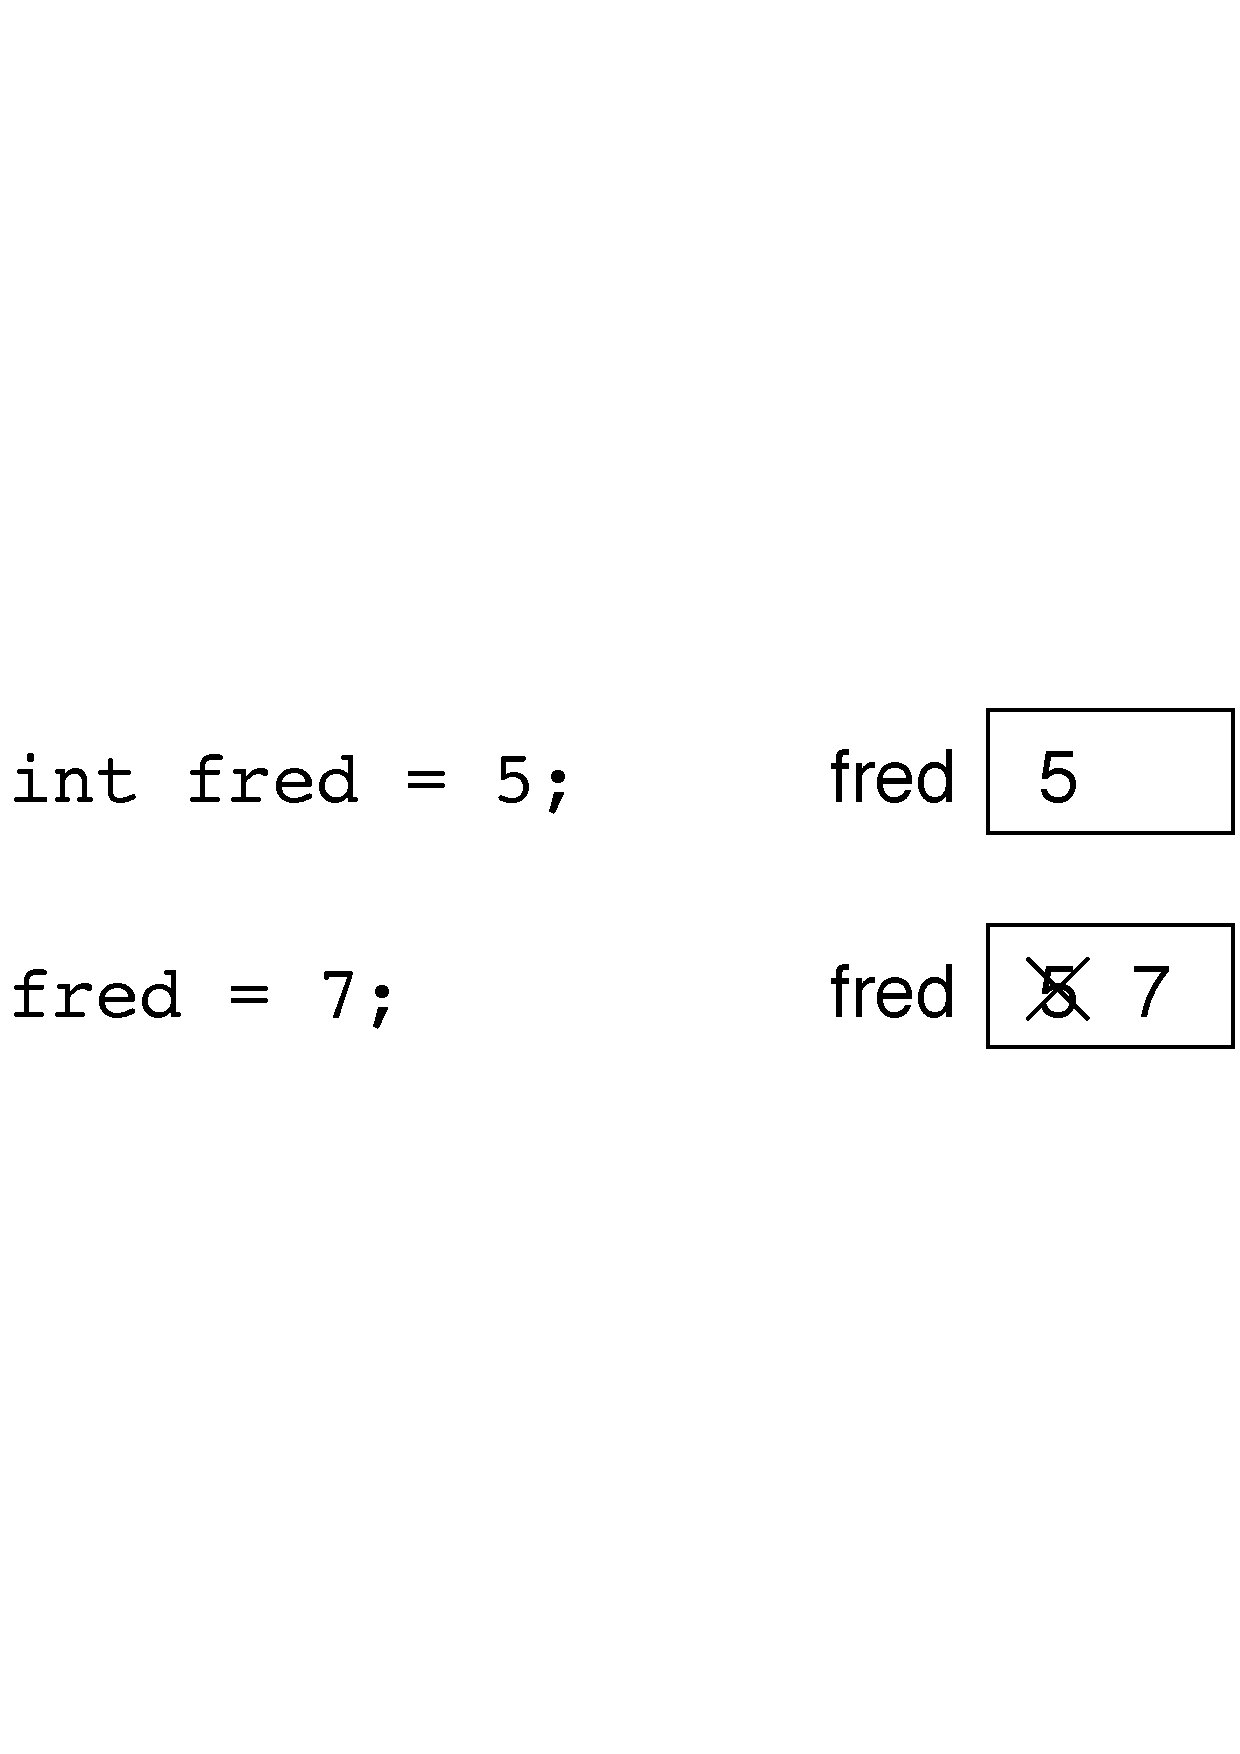
\includegraphics[height=1.8cm]{figs/assign2.pdf}}
\vspace{0.1in}

When there are multiple assignments to a variable, it is especially
important to distinguish between an assignment statement and a
statement of equality.  Because C uses the {\tt =} symbol for
assignment, it is tempting to interpret a statement like {\tt a = b}
as a statement of equality.  It is not! In many programming languages 
an alternate symbol is used
for assignment, such as {\tt <-} or {\tt :=}, in order to
avoid confusion.

First of all, equality is commutative, and assignment is not.
For example, in mathematics if $a = 7$ then $7 = a$.  But in
C the statement {\tt a = 7;} is legal, and {\tt 7 = a;}
is not.

Furthermore, in mathematics, a statement of equality is true
for all time.  If $a = b$ now, then $a$ will always equal $b$.
In C, an assignment statement can make two variables equal,
but they don't have to stay that way!

\begin{verbatim}
  int a = 5;
  int b = a;     /* a and b no have the same value*/
  a = 3;         /* a and b are no longer have the same value */
\end{verbatim}
%
The third line changes the value of {\tt a} but it does not
change the value of {\tt b}, and so they are no longer equal.

The ability to make multiple assignments to a variable means we can {\bf self assign} variables:

\begin{verbatim}
	  int a = 5;  
	  a = a + 1;       
\end{verbatim}
%
Assignment has the lowest precedent. 
This means that all other operations in the expression are evaluated before the assignment. 
In the first line code {\tt a} is initialized with a value of 5. In the second line, 
the expression  to the right of the assignment operator ($=$) is evaluated first. 
Since {\tt a} has the value 5, {\tt a + 1}  results in the value 6.
Finally we assign the result of 6 to {\tt a}..

\index{self assignment!operator}
\index{operator!self assignment}

Self assignment is actually very common. In fact, C has operators specifically for this task.
Several of these operators follow:

 \begin{verbatim}
 	int x = 3;
 	x += 2;				/* means x = x + 2 */      
 	x *= 4;				/* means x = x * 4  */      
 	x -= 6;				/* means x = x - 6  */      
 	x /= 6;				/* means x = x / 6   */    
 	x %=2;			 /* means x = x % 2 */  
 \end{verbatim}
 %
For a very specific set of self assignment, we have an even shorter way to write it. 
When we add one to a number, we call that incrementing. 
Decrementing means subtracting one from a number.
Incrementing and decrementing are so common they have 
their own operators $++$ for increment and $--$ for decrementing.

 \begin{verbatim}
  int x = 5;
  x++;         					 //add 1 to x
  printf("%i\n", x);	  //prints 6
   x--;         				 //sutracts 1 from x
  printf("%i\n", x);  	//prints 5
\end{verbatim}
%
 The increment/decrement operator can be placed before the variable (pre-increment/pre-decrement) or after the variable (post-increment/post-decrement). When using the pre-operators, the value is modified then utilized in an expression. When the post-operators are used, the value is utilized then modified. 
  \begin{verbatim}
  int x = 1;
  int y = 1;
  printf("%i\n", x++);  //prints 1, but x = 2 when completed
  printf("%i\n", ++y); //prints 2 and y = 2 when completed
  printf("%i\n", x);  //prints 2
  printf("%i\n", y);  //prints 2
 \end{verbatim}
 %
This behavior can be confusing and being careless with them can lead to errors. 
The best is to never mix the increment and decrement operators with other expressions. 
They should be executed on a line alone.
  \begin{verbatim}
	int x = 1;
	int y = 1;
	 x++;
	 ++y;
	printf("%i\n", x);  //prints 2
	printf("%i\n", y);  //prints 2
\end{verbatim}
%
\section{Iteration}
\index{iteration}

One of the things computers are often used for is the automation
of repetitive tasks.  Repeating identical or similar tasks without
making errors is something that computers do well and people do
poorly.

In section \ref{recursion} we have seen programs that use {\bf recursion} to perform
repetition, such as {\tt printLines()} and {\tt countdown()}. 
I now want to introduce a new
type of repetition, that is called {\bf iteration}, and C provides
several language features that make it easier to write repetitive
programs.

We introduce two new control structures,  the {\tt while}
statement and the {\tt for} statement. 
These are repetition structures - they repeat stuff.

\section{The {\tt while} statement}
\index{statement!while}
\index{while statement}

We can write {\tt countdown()} program using a {\tt while} statement:

\begin{verbatim}
  void countdown (int n) 
  {
      while (n > 0) 
      {
          printf ("%i\n", n);
          n = n-1;
      }
      printf ("Blastoff!\n");
  }
\end{verbatim}
%
You can almost read a {\tt while} statement as if it were
English.  What this means is, ``While {\tt n} is greater than
zero, continue displaying the value of {\tt n} and then reducing
the value of {\tt n} by 1.  When you get to zero, output the
word `Blastoff!'''

More formally, the flow of execution for a {\tt while} statement
is as follows:

 \begin{enumerate}
 	
 	\item Evaluate the condition in parentheses, yielding {\tt true}
or {\tt false}.

\item If the condition is false, exit the {\tt while} statement
and continue execution at the next statement.

\item If the condition is true, execute each of the statements
between the curly-brackets, and then go back to step 1.

\end{enumerate}

This type of flow is called a {\bf loop} because the third step loops
back around to the top.  Notice that if the condition is false the
first time through the loop, the statements inside the loop are
never executed.  The statements inside the loop are called
the {\bf body} of the loop.

\index{loop}
\index{loop!body}
\index{loop!infinite}
\index{body!loop}
\index{infinite loop}

The body of the loop should change the value of
one or more variables so that, eventually, the condition becomes
false and the loop terminates.  Otherwise the loop will repeat
forever, which is called an {\bf infinite loop}.  An endless
source of amusement for computer scientists is the observation
that the directions on shampoo, ``Lather, rinse, repeat,'' are
an infinite loop.

In the case of {\tt countdown()}, we can prove that the loop
will terminate because we know that the value of {\tt n} is
finite, and we can see that the value of {\tt n} gets smaller
each time through the loop (each {\bf iteration}), so
eventually we have to get to zero.  In other cases it is not
so easy to tell:

\begin{verbatim}
  void sequence (int n) 
  {
      while (n != 1) 
      {
          printf ("%i\n", n);
          if (n%2 == 0)       /* n is even */
          {          
              n = n / 2;
          } 
          else                /* n is odd */
          {                  
              n = n*3 + 1;
          }
      }
  }
\end{verbatim}
%
The condition for this loop is {\tt n != 1}, so the loop
will continue until {\tt n} is 1, which will make the condition
false.

At each iteration, the program outputs the value of {\tt n} and then
checks whether it is even or odd.  If it is even, the value of
{\tt n} is divided by two.  If it is odd, the value is replaced
by $3n+1$.  For example, if the starting value (the argument passed
to {\tt Sequence}) is 3, the resulting sequence is
3, 10, 5, 16, 8, 4, 2, 1.

Since {\tt n} sometimes increases and sometimes decreases, there is no
obvious proof that {\tt n} will ever reach 1, or that the program will
terminate.  For some particular values of {\tt n}, we can prove
termination.  For example, if the starting value is a power of two, then
the value of {\tt n} will be even every time through the loop, until
we get to 1.  The previous example ends with such a sequence,
starting with 16.

Particular values aside, the interesting question is whether
we can prove that this program terminates for {\em all} values of n.
So far, no one has been able to prove it {\em or} disprove it!

\section{Looping Design Patterns}
When learning about loops it is helpful to identify common design pattern.
We will first discuss the a basic strategy for writing loops and then detail a number of common loop patterns such as the counting loop, the user termination loop, the sentinel loop, and the value validation loop.

The while loop is the most universal loop, but any while loop to work properly, it needs three things:
\begin{enumerate}
	\item A variable with an initial value before the loop, this will be the test variable in the condition
	\item A conditional test on the variable at the start of the loop
	\item An assignment on the test variable inside the loop body
\end{enumerate}

All of these components are needed for a loop to work. Let's identify these pieces from one of our previous loops. 

\begin{verbatim}
	void countdown (int n) 
	{
		 //#1 n has an initial value when passed to the function
		  while (n > 0) //#2 this is a test on the variable
	 	{
		 	  printf ("%i\n", n);
		 	  n = n-1;  //#3 this is an assignment on the variable
	 	}
	 	printf ("Blastoff!\n");
	}
\end{verbatim}
%
\index{loops!counting}
Now that we have a basic strategy for laying out our while loops, let's examine some common patterns. The most common pattern we see it the {\bf counting loop}. This loop is used for iterating a specified number of times. If you can count the number of times you need your loop to run this may the pattern you need.

in a counting loop we start out counter with an initial value. Our condition will test if the count has yet to reach a specific limit. At each iteration we increment the count. 
\begin{verbatim}
		//#1 count has an initial value of zero
		int count = 0;
		
		while (count  < 10) //#2 this is a test on the variable, we will loop 10 times
		{
			 printf ("%i\n", count);  //do something in the loop
			 count++;   //#3 this is an assignment on the variable
		}
\end{verbatim}
%

\index{loops!sentinel}
Another common pattern we see it the {\bf sentinel loop}. A sentient is like a guard on watch. This loop will keep iterating until a special value is seen by the guard.  
\begin{verbatim}
 	int value;
 	puts("enter a grade from 0 to 100. Enter a negative number to stop");
 	scanf(" %i", &value);  //#1 get an intial value before the loop
	
 	while (value >= 0) //#2 test for a sentinel value
 	{
	  	printf ("%i\n", value);  //do something in the loop
		
	   //#3 this is an assignment on the variable - we need to prompt and scan again
	   puts("enter a grade from 0 to 100. Enter a negative number to stop");
	   scanf(" %i", &value);  //this is an assignment
 	}
\end{verbatim}
%
\index{loops!user-terminated}
We can look at another sentinel, but we will call this a {\bf user terminated loop}. Like our sentinel, this uses user input to end a program.
\begin{verbatim}
	char choice;
	puts("start a program y or n");
	scanf(" %c", &choice);  //#1 get an intial value before the loop
	
	while (choice == 'y') //#2 test for a sentinel value
	{
		/ /run a wholoe program
		
		 //#3 this is an assignment on the variable - we need to prompt and scan again
		
		 puts("Do you want to run the progam again");
		 scanf(" %c", &choice); 
	}
\end{verbatim}
%
\index{loops!value validation}
Our last looping pattern is the value validation pattern. If you need a user to enter a number a bounded value. You can use this loop to ensure a value fits your bound.  In this loop we ask the user for input until an 'y' or an 'n' is entered. All three of our loop components are here, unlabeled. Can you identify them?
\begin{verbatim}
	char choice;
	puts("start a program y or n");
	scanf(" %c", &choice);  
	while(choice != 'y' && choice != 'n')
	{
		puts("that is invalid input");
		puts("start a program y or n");
		scanf(" %c", &choice);  
	}	
//more program after this
\end{verbatim}
%

\section{Tables}
\index{table}
\index{logarithm}

One of the things loops are good for is generating
tabular data.  For example, before computers were readily available,
people had to calculate logarithms, sines and cosines, and other
common mathematical functions by hand.
To make that easier, there were books containing long tables
where you could find the values of various functions.
Creating these tables was slow and boring, and the result
tended to be full of errors.

When computers appeared on the scene, one of the initial reactions
was, ``This is great!  We can use the computers to generate the
tables, so there will be no errors.''  That turned out to be true
(mostly), but shortsighted.  Soon thereafter computers and
calculators were so pervasive that the tables became obsolete.

Well, almost.  It turns out that for some operations, computers
use tables of values to get an approximate answer, and then
perform computations to improve the approximation.  In some
cases, there have been errors in the underlying tables, most
famously in the table the original Intel Pentium used to perform
floating-point division.

\index{division!floating-point}

Although a ``log table'' is not as useful as it once was, it still
makes a good example of iteration.  The following program outputs a
sequence of values in the left column and their logarithms in the
right column:

\begin{verbatim}
  double x = 1.0;
  while (x < 10.0) 
  {
      printf ("%.0f\t%f\n", x ,log(x));
      x = x + 1.0;
  }
\end{verbatim}
%
The sequence \verb+\t+ represents a {\bf tab} character.
The sequence \verb+\n+ represents a newline character.  
They are so called \emph{escape sequences} which are used to encode
non-printable ASCII-characters.
Escape sequences can be included anywhere in a string, although in these examples
the sequence is the whole string.

A tab character causes the cursor to shift to the right until
it reaches one of the {\bf tab stops}, which are normally every
eight characters.  As we will see in a minute, tabs are useful
for making columns of text line up.
A newline character causes the cursor to move on to the next line.  
%Usually if a newline character appears by itself, I use {\tt endl}, but
%if it appears as part of a string, I use \verb+\n+.

The output of this program is:

\begin{verbatim}
   1      0.000000
   2      0.693147
   3      1.098612
   4      1.386294
   5      1.609438
   6      1.791759
   7      1.945910
   8      2.079442
   9      2.197225
\end{verbatim}
%
If these values seem odd, remember that the {\tt log()} function uses
base $e$.  Since powers of two are so important in computer science,
we often want to find logarithms with respect to base 2.  To do that,
we can use the following formula:

\[ \log_2 x = \frac {log_e x}{log_e 2} \]
%
Changing the output statement to

\begin{verbatim}
      printf ("%.0f\t%f\n", x, log(x) / log(2.0));
\end{verbatim}
%
yields:

\begin{verbatim}
    1      0.000000
    2      1.000000
    3      1.584963
    4      2.000000
    5      2.321928
    6      2.584963
    7      2.807355
    8      3.000000
    9      3.169925
\end{verbatim}
%
We can see that 1, 2, 4 and 8 are powers of two, because
their logarithms base 2 are round numbers.  If we wanted to find
the logarithms of other powers of two, we could modify the
program like this:

\begin{verbatim}
    double x = 1.0;
    while (x < 100.0) 
    {
        printf ("%.0f\t%.0f\n", x, log(x) / log(2.0));
        x = x * 2.0;
    }
\end{verbatim}
%
Now instead of adding something to {\tt x} each time through
the loop, which yields an arithmetic sequence, we multiply
{\tt x} by something, yielding a {\bf geometric} sequence.
The result is:

\begin{verbatim}
    1      0
    2      1
    4      2
    8      3
    16     4
    32     5
    64     6
\end{verbatim}
%
Because we are using tab characters between the columns, the
position of the second column does not depend on the number
of digits in the first column.

Log tables may not be useful any more, but for computer scientists,
knowing the powers of two is!  As an exercise, modify this program
so that it outputs the powers of two up to 65536
(that's $2^{16}$).  Print it out and memorize it.

\section{Two-dimensional tables}
\index{table!two-dimensional}

A two-dimensional table is a table where you choose a row and
a column and read the value at the intersection.  A multiplication
table is a good example.  Let's say you wanted to print a
multiplication table for the values from 1 to 6.

A good way to start is to write a simple loop that prints
the multiples of 2, all on one line.

\begin{verbatim}
    int i = 1;
    while (i <= 6) 
    {
        printf("%i   ", i*2);
        i = i + 1;
    }
    printf("\n");
\end{verbatim}
%
The first line initializes a variable named {\tt i}, which is
going to act as a counter, or {\bf loop variable}.  As the
loop executes, the value of {\tt i} increases from 1 to 6,
and then when {\tt i} is 7, the loop terminates.  Each
time through the loop, we print the value {\tt 2*i} followed
by three spaces.  By omitting the  \verb+\n+ from the
first output statement, we get 
all the output on a single line.

\index{loop variable}
\index{variable!loop}

The output of this program is:

\begin{verbatim}
    2   4   6   8   10   12
\end{verbatim}
%
So far, so good.  The next step is to {\bf encapsulate} and {\bf
generalize}.

\section {Encapsulation and generalization}

Encapsulation usually means taking a piece of code and wrapping it up
in a function, allowing you to take advantage of all the things functions
are good for.  We have seen two examples of encapsulation, when we
wrote {\tt PrintParity()} in Section~\ref{alternative} and {\tt
IsSingleDigit()} in Section~\ref{bool}.

Generalization means taking something specific, like printing
multiples of 2, and making it more general, like printing the
multiples of any integer.

\index{encapsulation}
\index{generalization}

Here's a function that encapsulates the loop from the previous
section and generalizes it to print multiples of {\tt n}.

\begin{verbatim}
    void PrintMultiples (int n)
    {
        int i = 1;
        while (i <= 6) 
        {
            printf("%i   ", i*n);
            i = i + 1;
        }
        printf("\n");
    }
\end{verbatim}
%
To encapsulate, all I had to do was add the first line,
which declares the name, parameter,
and return type.  To generalize, all I had to do was replace
the value 2 with the parameter {\tt n}.

If we call this function with the argument 2, we get the same
output as before.  With argument 3, the output is:

\begin{verbatim}
    3   6   9   12   15   18
\end{verbatim}
%
and with argument 4, the output is

\begin{verbatim}
    4   8   12   16   20   24 
\end{verbatim}
%
By now you can probably guess how we are going to print a
multiplication table: we'll call {\tt PrintMultiples()} repeatedly with
different arguments.  In fact, we are going to use another loop to
iterate through the rows.

\begin{verbatim}
    int i = 1;
    while (i <= 6) 
    {
        PrintMultiples (i);
        i = i + 1;
    }    
\end{verbatim}
%
First of all, notice how similar this loop is to the one inside {\tt
PrintMultiples()}.  I only replaced the call of the \texttt{printf()} function with 
the call of the \texttt{PrintMultiples()} function.

The output of this program is

\begin{verbatim}
    1   2   3   4   5   6   
    2   4   6   8   10   12   
    3   6   9   12   15   18   
    4   8   12   16   20   24   
    5   10   15   20   25   30   
    6   12   18   24   30   36   
\end{verbatim}
%
which is a (slightly sloppy) multiplication table.  If the
sloppiness bothers you, try replacing the spaces between
columns with tab characters and see what you get.

\section{Functions}
\index{function}

In the last section I mentioned ``all the things functions
are good for.''  About this time, you might be wondering
what exactly those things are.  Here are some of the reasons
functions are useful:

\begin{itemize}

\item By giving a name to a sequence of statements, you make
your program easier to read and debug.

\item Dividing a long program into functions allows you to
separate parts of the program, debug them in isolation, and
then compose them into a whole.

\item Functions facilitate both recursion and iteration.

\item Well-designed functions are often useful for many programs.
Once you write and debug one, you can reuse it.

\end{itemize}

\section{More encapsulation}
\index{encapsulation}
\index{program development!encapsulation}

To demonstrate encapsulation again, I'll take the code
from the previous section and wrap it up in a function:

\begin{verbatim}
    void PrintMultTable () 
    {
        int i = 1;
        while (i <= 6) 
        {
            PrintMultiples (i);
            i = i + 1;
        }
    }
\end{verbatim}
%
The process I am demonstrating is a common 
development plan.  You develop code gradually by adding
lines to {\tt main()} or someplace else, and then when you get
it working, you extract it and wrap it up in a function.

The reason this is useful is that you sometimes don't know
when you start writing exactly how to divide the program into
functions.  This approach lets you design as you go along.

\section{Local variables}

About this time, you might be wondering how we can use the same
variable {\tt i} in both {\tt PrintMultiples()} and {\tt
PrintMultTable()}.  Didn't I say that you can only declare a variable
once?  And doesn't it cause problems when one of the functions changes
the value of the variable?

The answer to both questions is ``no,'' because the {\tt i} in {\tt
PrintMultiples()} and the {\tt i} in {\tt PrintMultTable()} are
{\em not the same variable}.  They have the same name, but
they do not refer to the same storage location, and changing
the value of one of them has no effect on the other.

\index{local variable}
\index{variable!local}

Remember that variables that are declared inside a function definition
are local.  You cannot access a local variable from outside its
``home'' function, and you are free to have multiple variables with
the same name, as long as they are not in the same function.

The stack diagram for this program shows clearly that the
two variables named {\tt i} are not in the same storage location.
They can have different values, and changing one does not affect
the other.


\vspace{0.1in}
\centerline{\epsfig{figure=figs/stack4.pdf,width=6.5cm}}
\vspace{0.1in}
\index{stack diagram}
\index{diagram!stack}
%
Notice that the value of the parameter {\tt n} in
{\tt PrintMultiples()} has to be the same as the value
of {\tt i} in {\tt PrintMultTable()}.  On the other hand,
the value of {\tt i} in {\tt PrintMultiples()} goes
from 1 up to {\tt 6}.  In the diagram, it happens to be 3.
The next time through the loop it will be 4.

It is often a good idea to use different variable names in
different functions, to avoid confusion, but there are good
reasons to reuse names.  For example, it is common to
use the names {\tt i}, {\tt j} and {\tt k} as loop variables.
If you avoid using them in one function just because you
used them somewhere else, you will probably make the program
harder to read.

\index{loop variable}
\index{variable!loop}

%%
\section{More generalization}
\label{More generalization}
\index{generalization}

As another example of generalization, imagine you wanted
a program that would print a multiplication table of any
size, not just the 6x6 table.  You could add a parameter to
{\tt PrintMultTable()}:

\begin{verbatim}
    void PrintMultTable (int high) 
    {
        int i = 1;
        while (i <= high) 
        {
            PrintMultiples (i);
            i = i + 1;
        }
    }
\end{verbatim}
%
I replaced the value 6 with the parameter {\tt high}.  If I
call {\tt PrintMultTable()} with the argument 7, I get:

\begin{verbatim}
    1   2   3   4   5   6   
    2   4   6   8   10   12   
    3   6   9   12   15   18   
    4   8   12   16   20   24   
    5   10   15   20   25   30   
    6   12   18   24   30   36   
    7   14   21   28   35   42   
\end{verbatim}
%
which is fine, except that I probably want the table to
be square (same number of rows and columns), which means
I have to add another parameter to {\tt PrintMultiples()},
to specify how many columns the table should have.

Just to be annoying, I will also call this parameter {\tt high},
demonstrating that different functions can have parameters
with the same name (just like local variables):

\begin{verbatim}
  void PrintMultiples (int n, int high) 
  {
      int i = 1;
      while (i <= high) 
      {
          printf ("%i    ", n*i);
          i = i + 1;
      }    
      printf ("\n");
  }

  void PrintMultTable (int high) 
  {
      int i = 1;
      while (i <= high) 
      {
          PrintMultiples (i, high);
          i = i + 1;
      }
  }
\end{verbatim}
%
Notice that when I added a new parameter, I had to change the first
line of the function, and I also had to
change the place where the function is called in {\tt PrintMultTable()}.
As expected, this program generates a square 7x7 table:

\begin{verbatim}
    1   2   3   4   5   6   7   
    2   4   6   8   10   12   14   
    3   6   9   12   15   18   21   
    4   8   12   16   20   24   28   
    5   10   15   20   25   30   35   
    6   12   18   24   30   36   42   
    7   14   21   28   35   42   49
\end{verbatim}
%
When you generalize a function appropriately, you often find
that the resulting program has capabilities you did not intend.
For example, you might notice that the multiplication table
is symmetric, because $ab = ba$, so all the entries in the
table appear twice.  You could save ink by printing only
half the table.  To do that, you only have to change one
line of {\tt PrintMultTable()}.  Change

\begin{verbatim}
      PrintMultiples (i, high);
\end{verbatim}
%
to

\begin{verbatim}
      PrintMultiples (i, i);
\end{verbatim}
%
and you get:

\begin{verbatim}
    1   
    2   4   
    3   6   9   
    4   8   12   16   
    5   10   15   20   25   
    6   12   18   24   30   36   
    7   14   21   28   35   42   49  
\end{verbatim}
%
I'll leave it up to you to figure out how it works.

\section{Glossary}

\begin{description}

\item[loop:]  A statement that executes repeatedly while a
condition is true or until some condition is satisfied.

\item[infinite loop:]  A loop whose condition is always true.

\item[body:]  The statements inside the loop.

\item[iteration:]  One pass through (execution of) the body
of the loop, including the evaluation of the condition.

\item[tab:] A special character, written as \verb+\t+ in C,
that causes the cursor to move to the next tab stop on the
current line.

\item[encapsulate:]  To divide a large complex program into
components (like functions) and isolate the components from
each other (for example, by using local variables).

\item[local variable:]  A variable that is declared inside
a function and that exists only within that function.  Local variables
cannot be accessed from outside their home function, and do not
interfere with any other functions.

\item[generalize:]  To replace something unnecessarily specific
(like a constant value) with something appropriately general
(like a variable or parameter).  Generalization makes code more
versatile, more likely to be reused, and sometimes even easier
to write.

\item[development plan:]  A process for developing a program.
In this chapter, I demonstrated a style of development based on
developing code to do simple, specific things, and then encapsulating
and generalizing.

\index{loop}
\index{infinite loop}
\index{body}
\index{tab}
\index{loop!infinite}
\index{iteration}
\index{encapsulation}
\index{generalization}
\index{local variable}
\index{variable!local}
\index{program development}

\end{description}

\section{Exercises}
\setcounter{exercisenum}{0}

% LaTeX source for textbook ``How to think like a computer scientist''
% Copyright (C) 1999  Allen B. Downey
% Copyright (C) 2009  Thomas Scheffler

%%%%%%%%%%%%%%%%%%%%%%%%%%%%%%%%%%%%%%

\begin{exercise}\label{infloop}
%changed the condition on the loop so that it will terminate
%(was this *supposed* to be an infinite loop?)
\begin{verbatim}
    void loop(int n) 
    {
        int i = n;
        while (i > 1) 
        {
            printf ("%i\n",i);
            if (i%2 == 0) 
            {
                i = i/2;
            } 
            else 
            {
                i = i+1;
            }
        }
    }

    int main (void) 
    {
        loop(10);
        return EXIT_SUCCESS;
    }
\end{verbatim}
%
\begin{enumerate}

\item  Draw a table that shows the value of the variables {\tt i} and {\tt n} during the execution of the program. 
The table should contain one column for each variable and one line for each iteration.


\item What is the output of this program?

\end{enumerate}
\end{exercise}

%%%%%%%%%%%%%%%%%%%%%%%%%%%%%%%%%%%%%%


\begin{exercise}
In Exercise~\ref{ex.power} we wrote a recursive version of {\tt
power()}, which takes a double {\tt x} and an integer {\tt n} and
returns $x^n$.  Now write an iterative function to perform the same
calculation.
\end{exercise}

%%%%%%%%%%%%%%%%%%%%%%%%%%%%%%%%%%%%%%



\begin{exercise}
	Define a function and prototype called getFirstNumber(). This function takes no parameters and returns an integer. The function should prompt a user for a number between 1 and 10. Use a loop to validate the input's value. If the value is invalid, continue to prompt until a valid value is received. When a valid value is given, it should be returned from the function
	
	Define a function and prototype called getSecondNumber(). This function takes one integer parameter and returns an integer. The parameter is a lower bound for a number. The function should prompt a user for a number between the lower bound and 15. Use a loop to validate the input's value. If the value is invalid, continue to prompt until a valid value is received. When a valid value is given, it should be returned from the function
	
	Define a function and prototype called printRange. This function takes two integer parameters, the lower and upper bound) and returns void. The function should use to print all the numbers form the lower to upper bound.
	
	Write a main program that calls the getFirstNumber function and uses the result as input to the getSecondNumber function. These will be the lower and upper bound for calling printRange, call print range with this input
	
	The goal of this exercise is to practice various loop patterns and practice using functions. 
\end{exercise}

%%%%%%%%%%%%%%%%%%%%%%%%%%%%%%%%%%%%%%


\begin{exercise}
	Write a program that meets the following description. 
	The user is asked if they want to play a game. If so the program should generate a random number between 1 and 10. This is the secret number. Prompt the user to make a guess at the secret number. Allow the to make 3 guesses. The game ends it the user guesses correctly or if they run out of guesses. Once the game is over, ask the user if they want to play again and replay the game.
	
	It is up to you to use the best loop designs for this problem. Be sure to use functions (can you reuse any functions you previously wrote)
	
	The goal of this exercise is to practice program design and loop types.
\end{exercise}

%%%%%%%%%%%%%%%%%%%%%%%%%%%%%%%%%%%%%%


%% LaTeX source for textbook ``How to think like a computer scientist''
% Copyright (C) 1999  Allen B. Downey
% Copyright (C) 2009  Thomas Scheffler


\chapter{Arrays}
\label{arrays}
\index{arrays}
\index{type!array}

A {\bf array} is a set of values where each value is identified and referenced by a
number (called an index).  The nice thing
about arrays is that they can be made up of any type of element,
including basic types like {\tt int}s and {\tt double}s, 
but all the values in an array have to have the same type.
%and user-defined types like {\tt Point} and {\tt Time}.


When you declare an array, you have to determine the number of
elements in the array. Otherwise the declaration looks similar to other variable types:

\begin{verbatim}
    int c[4];
    double values[10];
\end{verbatim}


%

Syntactically, array variables look like other C variables except that they are followed 
by {\tt [NUMBER\_OF\_ELEMENTS]}, the number of elements in the array enclosed in square brackets. 
The first line in our example, {\tt int c[4];} is of the type "array of integers" and creates a array of four integers named {\tt c}.
The second line, {\tt double values[10];} has the type "array of doubles" and
  creates an array of 10 {\tt double}s. 

%The number
%of elements in {\tt values} depends on {\tt size}. You can use any
%integer expression to determine the size of an array.
%!!! Not in C
%this would be dynamic arrays, that can not be initialised at definition time!!!

%

C allows you to to initialize the element values of an array immediately
after you have declared it.  The values  for the individual elements must be 
enclosed in curly brackets {\tt \{\}} and separated by comma, as in the following example:

\begin{verbatim}
    int c[4] = {0, 0, 0, 0};
\end{verbatim}

This statement creates an array of four elements and initializes
all of them to zero.
This syntax is only legal at initialisation time. Later in your program you can only
assign values for the array element by element.

%
The following figure shows how arrays are represented in state
diagrams:

%\myfig{figure=figs/array.eps}

\unitlength0.1cm

\begin{picture}(40,10)(-30,-5)
%\put(-4,1.5){{\Large \texttt{c}}}
%\put(0,1.5){\framebox(2,2)}
%\thicklines
%\put(2,2.5){\vector(1,0){8}}
%\thinlines
\put(5,1.5){{\Large \texttt{c}}}
\put(10,0){\framebox(7,5){\textbf{\textsf{0}}}}
\put(17,0){\framebox(7,5){\textbf{\textsf{0}}}}
\put(24,0){\framebox(7,5){\textbf{\textsf{0}}}}
\put(31,0){\framebox(7,5){\textbf{\textsf{0}}}}

\put(10.5,-4){{\scriptsize \texttt{c[0]}}}
\put(17.5,-4){{\scriptsize \texttt{c[1]}}}
\put(24.5,-4){{\scriptsize \texttt{c[2]}}}
\put(31.5,-4){{\scriptsize \texttt{c[3]}}}

\end{picture}

The large numbers inside the boxes are the values of the {\bf elements} in
the array.  The small numbers outside the boxes are the
indices used to identify each box.  When you allocate a new
array, without initializing, the arrays elements typically
contain arbitrary values and you must initialize them to
a meaningful value before using them.

%%
\section{Accessing elements}
\index{element}
\index{array!element}

The {\tt []} operator allows us to read and write the individual elements of an array.  
The indices start at zero, so {\tt c[0]}
refers to the first element of the array, and {\tt c[1]}
refers to the second element.  You can use the {\tt []} operator
anywhere in an expression:


\begin{verbatim}
    c[0] = 7;
    c[1] = c[0] * 2;
    c[2]++;
    c[3] -= 60;
\end{verbatim}
%
All of these are legal assignment statements.  Here is the
effect of this code fragment:


%\myfig{figure=figs/array2.eps}

\unitlength0.1cm

\begin{picture}(40,10)(-30,-5)
%\put(-11,1.5){\texttt{count}}
%\put(0,1.5){\framebox(2,2)}
%\thicklines
%\put(2,2.5){\vector(1,0){8}}
%\thinlines
\put(5,1.5){{\Large \texttt{c}}}

\put(10,0){\framebox(7,5){\textbf{\textsf{7}}}}
\put(17,0){\framebox(7,5){\textbf{\textsf{14}}}}
\put(24,0){\framebox(7,5){\textbf{\textsf{1}}}}
\put(31,0){\framebox(7,5){\textbf{\textsf{-60}}}}

\put(10.5,-4){{\scriptsize \texttt{c[0]}}}
\put(17.5,-4){{\scriptsize \texttt{c[1]}}}
\put(24.5,-4){{\scriptsize \texttt{c[2]}}}
\put(31.5,-4){{\scriptsize \texttt{c[3]}}}

\end{picture}

By now you should have noticed that the four elements of this array
are numbered from 0 to 3, which means that there is no element with
the index 4.  

Nevertheless, it is a common error to go
beyond the bounds of an array. In safer languages such as Java, this will cause an 
error and most likely the program quits. C does not check array boundaries, so
your program can go on accessing memory locations beyond the array itself, as if 
they where part of the array. This is most likely wrong and can cause very
severe bugs in your program. 
\begin{quote}

{\bf It is necessary that you, as a programmer,
make sure that your code correctly observes array boundaries!}

\end{quote}




\index{run-time error}
\index{index}
\index{expression}

You can use any expression as an index, as long as it has type {\tt
int}.  One of the most common ways to index an array is with a loop
variable.  For example:

\begin{verbatim}
    int i = 0;
    while (i < 4) 
    {
        printf ("%i\n", c[i]);
        i++;
    }
\end{verbatim}

%
This is a standard {\tt while} loop that counts from 0
up to 4, and when the loop variable {\tt i} is 4, the
condition fails and the loop terminates.  Thus, the body
of the loop is only executed when {\tt i} is 0, 1, 2 and 3.

\index{loop}
\index{loop variable}
\index{variable!loop}

Each time through the loop we use {\tt i} as an index into
the array, printing the {\tt i}th element.  This type of
array traversal is very common.  Arrays and loops go together
like fava beans and a nice Chianti.

\index{fava beans}
\index{Chianti}

%%
\section{Copying arrays}
\index{array!copying}

Arrays can be a very convenient solution for a number of problems, like
storing and processing large sets of data.

However, there is very little that C does automatically for you. For example
you can not set all the elements of an array at the same time and you can not
assign one array to the other, even if they are identical in type and number of elements.


\begin{verbatim}
    double a[3] = {1.0, 1.0, 1.0};
    double b[3];

    a = 0.0;     /* Wrong! */
    b = a;       /* Wrong! */
\end{verbatim}
%

In order to set all of the elements of an array to some value, you must do so element by element.
To copy the contents of one array to another, you must again do so, by copying each element from
one array to the other.

\begin{verbatim}
    int i = 0;
    while (i < 3) 
    {
        b[i] = a[i];
        i++;
    }
\end{verbatim}

%%
\section{{\tt for} loops}

The loops we have written so far have a number of elements
in common.  All of them start by initializing a variable;
they have a test, or condition, that depends on that variable;
and inside the loop they do something to that variable,
like increment it.

\index{loop!for}
\index{for}
\index{statement!for}

This type of loop is so common that there is an alternate
loop statement, called {\tt for}, that expresses it more
concisely.  The general syntax looks like this:

\begin{verbatim}
    for (INITIALIZER; CONDITION; INCREMENTOR) 
    {
        BODY
    }
\end{verbatim}
%
This statement is exactly equivalent to

\begin{verbatim}
    INITIALIZER;
    while (CONDITION) 
    {
        BODY
        INCREMENTOR
    }
\end{verbatim}
%
except that it is more concise and, since it puts all the
loop-related statements in one place, it is easier to read.
For example:

\begin{verbatim}
    int i;
    for (i = 0; i < 4; i++) 
    {
        printf("%i\n", c[i]);
    }
\end{verbatim}
%
is equivalent to 

\begin{verbatim}
    int i = 0;
    while (i < 4) 
    {
        printf("%i\n", c[i]);
        i++;
    }
\end{verbatim}

%%
\section{Array length}
\label{Array length}
\index{length!array}
\index{array!length}
\index{sizeof}
\index{operator!sizeof}

C does not provide us with a convenient way to determine the
actual length of an array. Knowing the size of an array would
be convenient when we are looping through all elements of
the array and need to stop with the last element.

In order to determine the array length we could use the {\tt sizeof()} 
operator, that calculates the size of data types in bytes.
Most data types in C use more than one byte to store their values,
therefore it becomes necessary to divide the byte-count for the array by 
the byte-count for a single element to establish the number of elements
in the array.
\begin{verbatim}
    sizeof(ARRAY)/sizeof(ARRAY_ELEMENT)
\end{verbatim}

It is a good idea to use this value as the upper bound of a loop,
rather than a constant.  That way, if the size of the array
changes, you won't have to go through the program changing all the
loops; they will work correctly for any size array.

\begin{verbatim}
    int i, length;
    length = sizeof (c) / sizeof (c[0]);

    for (i = 0; i < length; i++) 
    {
        printf("%i\n", c[i]);
    }
\end{verbatim}
%
The last time the body of the loop gets executed, the value of {\tt i}
is {\tt length - 1}, which is the index of the last element.  When
{\tt i} is equal to {\tt length}, the condition fails and the body
is not executed, which is a good thing, since it would access a
memory location that is not part of the array.


%%
\pagebreak
\section{Arrays and random}
\index{statistics}
\index{distribution}
\index{mean}

The numbers generated by {\tt rand()} are supposed to be distributed
uniformly.  That means that each value in the range should be
equally likely.  If we count the number of times each value appears,
it should be roughly the same for all values, provided that we
generate a large number of values.

In the next few sections, we will write programs that generate
a sequence of random numbers and check whether this property
holds true.

%%
\section{Array of random numbers}
\label{Array of random numbers}

The first step is to generate a large number of random values
and store them in a array.  By ``large number,'' of course,
I mean 20.  It's always a good idea to start with a manageable
number, to help with debugging, and then increase it later.

The following function takes three arguments, an array of integers, 
the size of the array and an upper bound for the random values.  
It fills the array of {\tt int}s with random values between 0 and {\tt upperBound-1}.

\begin{verbatim}
    void RandomizeArray (int array[], int length, int upperBound) 
    {
        int i;
        for (i = 0; i < length; i++) 
        {
            array[i] = rand() % upperBound;
        }
    }
\end{verbatim}
%
The return type is {\tt void}, which means that
this function does not return any value to the calling function.
To test this function, it is convenient to have a function that
outputs the contents of a array.

\begin{verbatim}
    void PrintArray (int array[], int length) 
    {
        int i;
        for (i = 0; i < length; i++) 
        {
            printf ("%i ",  array[i]);
        }
    }
\end{verbatim}
%
The following code generates an array filled with random values and outputs it:

\begin{verbatim}
    int r_array[20];
    int upperBound = 10;
    int length = sizeof(r_array) / sizeof(r_array[0]);
  
    RandomizeArray (r_array, length, upperBound);
    PrintArray (r_array, length);
\end{verbatim}

%
On my machine the output is:

\begin{verbatim}
3 6 7 5 3 5 6 2 9 1 2 7 0 9 3 6 0 6 2 6 
\end{verbatim}
\nopagebreak%
which is pretty random-looking.  Your results may differ.

If these numbers are really random,
we expect each digit to appear the same number of times---twice
each.  In fact, the number 6 appears five times, and the numbers 4
and 8 never appear at all.

Do these results mean the values are not really uniform?  It's
hard to tell.  With so few values, the chances are slim
that we would get exactly what we expect.  But as the number
of values increases, the outcome should be more predictable.

To test this theory, we'll write some programs that count the
number of times each value appears, and then see what happens
when we increase the number of elements in our array.

%%
\section{Passing an array to a function}
\label{Passing an array to a function}
\index{call by reference}
\index{call by value}
\index{array parameters}
You probably have noticed that our {\tt RandomizeArray()} function 
looked a bit unusual. We pass an array to this function and expect 
to get a a randomized array back. Nevertheless, we have declared it to 
be a {\tt void} function, and miraculously the function appears to have 
altered the array.

This behaviour goes against everything what I have said about the
use of variables in functions so far.
C typically uses the so called {\bf call-by-value} evaluation of
expressions. If you pass a value to a function it gets copied from
the calling function to a variable in the called function. The same
is true if the function returns a value.
Changes to the internal variable in the called function do not affect the external 
values of the calling function.

When we pass an array to a function this behaviour changes to
something called {\bf call-by-reference} evaluation.
C does not copy the array to an internal array --  it rather generates a
reference to the original array and any operation in the called function 
directly affects the original array.
This is also the reason why we do not have to return anything from our 
function. The changes have already taken place. 

Call by reference also makes it necessary to supply the length of
the array to the called function, since invoking  the {\tt sizeof}
operator in the called function would determine the size of the reference
and not the original array.

%!!!Reference to later chapter needed!!!
We will further discuss call by reference and call by value in 
Section~\ref{Pointers and Addresses}, Section~\ref{Call by value} and
\ref{Call by reference}.

%%
\section{Counting}
\label{counting}
\index{traverse!counting}
\index{loop!counting}
\index{counter}

A good approach to problems like this is to think of simple functions
that are easy to write, and that might turn out to be useful.  Then
you can combine them into a solution.  This approach is sometimes
called {\bf bottom-up design}.  

Of course, it is not easy to
know ahead of time which functions are likely to be useful, but as you
gain experience you will have a better idea.
\index{bottom-up design}
\index{program development!bottom-up}
Also, it is not always obvious what sort of things are easy to write,
but a good approach is to look for subproblems that fit a pattern you
have seen before.

\index{pattern!counter}

%Back in Section~\ref{loopcount} we looked at a loop that traversed a
%string and counted the number of times a given letter appeared.  
In our current example we want to examine a potentially large set
of elements and count the number of times a certain value appears.
You
can think of this program as an example of a pattern called ``traverse
and count.''  The elements of this pattern are:

\begin{itemize}

\item A set or container that can be traversed, like a string
or a array.

\item A test that you can apply to each element in the container.

\item A counter that keeps track of how many elements pass
the test.

\end{itemize}

In this case, I have a function in mind called {\tt HowMany()} that
counts the number of elements in a array that are equal to a given value.
The parameters are the array, the length of the array and the integer value we are looking
for.  The return value is the number of times the value appears.

\begin{verbatim}
    int HowMany (int array[], int length, int value) 
    {
        int i; 
        int count = 0;
  
        for (i=0; i < length; i++) 
            {
                if (array[i] == value) count++;
            }
        return count;
    }
\end{verbatim}


\section{Checking the other values}

{\tt HowMany()} only counts the occurrences of a particular value, and
we are interested in seeing how many times each value appears.
We can solve that problem with a loop:

\begin{verbatim}
    int i;
    int r_array[20];
    int upperBound = 10;
    int length = sizeof(r_array) / sizeof(r_array[0]);
  
    RandomizeArray(r_array, length, upperBound);

    printf ("value\tHowMany\n");
    for (i = 0; i < upperBound; i++) 
    {
        printf("%i\t%i\n", i, HowMany(r_array, length, i));
    }
\end{verbatim}
%

%! ! ! Applies only to C++! ! !
%Notice that it is legal to declare a variable inside a {\tt for}
%statement.  This syntax is sometimes convenient, but you should
%be aware that a variable declared inside a loop only exists
%inside the loop.  If you try to refer to {\tt i} later, you
%will get a compiler error.

This code uses the loop variable as an argument to
{\tt HowMany()}, in order to check each value between 0 and 9,
in order.  The result is:

\begin{verbatim}
value   HowMany
0       2
1       1
2       3
3       3
4       0
5       2
6       5
7       2
8       0
9       2
\end{verbatim}
%
Again, it is hard to tell if the digits are really appearing
equally often.  If we increase the size of the array to 100,000 we
get the following:

\begin{verbatim}
value   HowMany
0       10130
1       10072
2       9990
3       9842
4       10174
5       9930
6       10059
7       9954
8       9891
9       9958
\end{verbatim}
%
In each case, the number of appearances is within about 1\% of
the expected value (10,000), so we conclude that the random
numbers are probably uniform.

\section {A histogram}
\index{histogram}

It is often useful to take the data from the previous tables
and store them for later access, rather than just print them.
What we need is a way to store 10 integers.  We could create
10 integer variables with names like {\tt howManyOnes},
{\tt howManyTwos}, etc.  But that would require a lot of
typing, and it would be a real pain later if we decided to
change the range of values.

A better solution is to use a array with length 10.  That
way we can create all ten storage locations at once and we
can access them using indices, rather than ten different names.
Here's how:

\begin{verbatim}
    int i;
    int upperBound = 10;
    int r_array[100000];
    int histogram[upperBound];
    int r_array_length = sizeof(r_array) / sizeof(r_array[0]);
  
    RandomizeArray(r_array, r_array_length, upperBound);

    for (i = 0; i < upperBound; i++) 
    {
        int count = HowMany(r_array, length, i);
        histogram[i] = count;
    }  
\end{verbatim}
%
I called the array {\bf histogram} because that's
a statistical term for a array of numbers that counts the
number of appearances of a range of values.

\index{histogram}

The tricky thing here is that I am using the loop variable
in two different ways.  First, it is an argument to {\tt HowMany()},
specifying which value I am interested in.  Second, it is
an index into the histogram, specifying which location I should
store the result in.

\section{A single-pass solution}

Although this code works, it is not as efficient as it could
be.  Every time it calls {\tt HowMany()}, it traverses the
entire array.  In this example we have to traverse the
array ten times!

It would be better to make a single pass through the array.
For each value in the array we could find the corresponding
counter and increment it.  In other words, we can use the
value from the array as an index into the histogram.  Here's
what that looks like:

\begin{verbatim}
    int upperBound = 10;
    int histogram[upperBound] = {0, 0, 0, 0, 0, 0, 0, 0, 0, 0};

    for (i = 0; i < r_array_length; i++) 
    {
        int index = r_array[i];
        histogram[index]++;
    }
\end{verbatim}
%
The second line initializes the elements of the histogram to
zeroes.  That way, when we use the increment
operator ({\tt ++}) inside the loop, we know we are starting from zero.
Forgetting to initialize counters is a common error.

As an exercise, encapsulate this code in a function called {\tt Histogram()} 
that takes an array and the range of values in the array
(in this case 0 through 10) as two parameters \texttt{min} and \texttt{max}. 
You should pass a second array to the function where a histogram of the
values in the array can be stored.


\section{Partially filled arrays}
In C, an array's sized is fixed at the moment it is declared. But what if we don't know how much space is needed when an array is declared. For example, we may want to store the names of students who enrolled in a course, but we don't know how many students there will be until they register. Or we may want to store some numbers that are entered by the user, but we don't know how many numbers there will be until they stop entering them. In these cases, we can use a {\bf partially filled array}.

A partially filled array is an array that has some empty slots that are not used for storing data. For example, if we declare an array of size 10, but only use 5 elements to store some data, then we have a partially filled array with 5 empty slots. The advantage of using a partially filled array is that we can allocate more space than we need at first, and then fill it up later as needed. The disadvantage is that we may waste some memory if we allocate too much space than we need.

To work with partially filled arrays in C, we need two things: a variable that defines the maximum size of the array (its capacity), and a local variable that keeps track of how many elements are actually used in the array (usually called size). The size variable also allows us to ensure that we don't exceed the capacity of the array when adding new elements. All the values are stored contiguously in the array starting at the zero index. This means we can use the size variable to find the next open location. We can assign a value at that location, then increase the size.

\begin{verbatim}

 #define CAPACITY  10  //the maximum size of the array

 int arr[CAPACITY]; // Declare an int array with the max capacity 

 int size = 0;  //the current size of the filled part

 //get some values from the user using a user-terminated loop (or sentinel loop)

 int num;
 puts("Enter some numbers (enter -1 to stop):");
 scanf("%d", &num);

 //while the user enters a valid number 
 //and we have room in the array
 while (num != -1 && size < CAPACITY) 
 {
	  arr[size] = num; 	
	  size++;  

	  puts("Enter some numbers (enter -1 to stop):");
	  scanf("%d", &num); // Read another number from input
 }
\end{verbatim}
%

\section{Glossary}

\begin{description}

\item[array:]  A named collection of values, where all the
values have the same type, and each value is identified by
an index.

\item[element:]  One of the values in a array.  The {\tt []}
operator selects elements of a array.

\item[index:]  An integer variable or value used to indicate
an element of a array.

\item[increment:]  Increase the value of a variable by one.
The increment operator in C is {\tt ++}. 

\item[decrement:]  Decrease the value of a variable by one.
The decrement operator in C is {\tt -}{\tt -}.

\item[bottom-up design:]  A method of program development that
starts by writing small, useful functions and then assembling
them into larger solutions.

\item[histogram:]  A array of integers where each integer
counts the number of values that fall into a certain range.

\index{array}
\index{element}
\index{index}
\index{deterministic}
\index{histogram}

\end{description}

%%
\section{Exercises}
\setcounter{exercisenum}{0}


% LaTeX source for textbook ``How to think like a computer scientist''
% Copyright (C) 1999  Allen B. Downey
% Copyright (C) 2009  Thomas Scheffler

%%%%%%%%%%%%%%%%%%%%%%%%%%%%%%%%%%%%%%
\begin{exercise}
	
	It helpful to have a function that prints the contents of an array. Define a function and prototype for a function called printIntArray that has 2 parameters, an int for the size of the array and an array of integers. Use a loop to print the contents of the array in a nicely formatted way. Write a main program that defines two arrays and use the function to print the arrays.  Below is an example output of the program:
	
	\begin{verbatim}
		[ 2, 5, 7, 8, 1 ]
		[ 1, 2, 9, 1 ]
	\end{verbatim}
	
\end{exercise}

%%%%%%%%%%%%%%%%%%%%%%%%%%%%%%%%%%%%%%
\begin{exercise}

A friend of yours shows you the following method and
explains that if {\tt number} is any two-digit number, the program
will output the number backwards.  He claims that if {\tt number} is
17, the method will output {\tt 71}.

Is he right?  If not, explain what the program actually does and
modify it so that it does the right thing.

\begin{verbatim}
   #include <stdio.h>
   #include<stdlib.h>
   
   int main (void)
   {
     int number = 71;
     int lastDigit = number%10;
     int firstDigit = number/10;
     printf("%i",lastDigit + firstDigit);
     return EXIT_SUCCESS;
  }

\end{verbatim}
%%%%%%%%%%%%%%%%%%%%%%%%%%%%%%%%%%%%%%

\end{exercise}
\begin{exercise}
	
	Rewrite the previous program so that it prompts the user for a three digit integer. Create a 3 element array and store each digit into the array. Use your printIntArray function to print the content of the array.
\end{exercise}


%%%%%%%%%%%%%%%%%%%%%%%%%%%%%%%%%%%%%%
\begin{exercise}
Write a function and prototype that takes an array of integers, the length of the array and an integer named
{\tt target} as arguments. 

The function should search through the provided array and should return the first index where
{\tt target} appears in the array, if it does. If {\tt target} is not in the array the function should 
return an invalid index value to indicate an error condition  (e.g.  -1).

Write a main program to test the function. Be sure to print the array as well.
\end{exercise}

%%%%%%%%%%%%%%%%%%%%%%%%%%%%%%%%%%%%%%

%%%%%%%%%%%%%%%%%%%%%%%%%%%%%%%%%%%%%%
\begin{exercise}
	Write a function and prototype that takes an array of integers, and the length of the array.
	
	The function should sum all the values in the array and then return the sum of the array. If the array is empty, return 0.
	
	Write a main program that creates a 20 element array, and uses a user-terminated loop to ask the user to fill the array with positive numbers. The user can stop the loop by entering a negative number. Use the array, call your function and print the resulting sum. Be sure to print the array as well/
\end{exercise}

%%%%%%%%%%%%%%%%%%%%%%%%%%%%%%%%%%%%%%
\begin{exercise}

One not-very-efficient way to sort the elements of an array
is to find the largest element and swap it with the first
element, then find the second-largest element and swap it with
the second, and so on.

\begin{enumerate}

\item Write a function called {\tt IndexOfMaxInRange()} that 
takes an array of integers, finds the
largest element in the given range, and returns its {\em index}.

\item Write a function called {\tt SwapElement()} that takes an
array of integers and two indices, and that swaps the elements
at the given indices.

\item Write a function called {\tt SortArray()} that takes an array of
integers and that uses {\tt IndexOfMaxInRange()} and {\tt SwapElement()}
to sort the array from largest to smallest.

\end{enumerate}
\end{exercise}


%%%%%%%%%%%%%%%%%%%%%%%%%%%%%%%%%%%%%%





%% LaTeX source for textbook ``How to think like a computer scientist''
% Copyright (C) 1999  Allen B. Downey
% Copyright (C) 2009  Thomas Scheffler
% Copyright (C) 2023  Michael Penta

\selectlanguage{english}
\chapter{Strings and things}
\label{strings}

\section{Containers for strings}

We have seen four types of values---characters, integers,
floating-point numbers and strings---but only three types of
variables---{\tt char}, {\tt int} and {\tt double}.  So
far we have no way to store a string in a variable or perform
operations on strings.

This chapter is going to rectify this situation and I can now tell
you that strings in C are stored as an array of characters terminated by the 
character {\tt \textbackslash 0}.

By now this explanation should make sense to you and you probably understand
why we had to learn quite a bit about the working of the language 
before we could turn our attention towards string variables.

\index{<string.h>}
\index{header file!string.h}
In the previous chapter we have seen that operations on arrays have 
only minimal support from the C language itself and we had
to program extra functions by ourselves.
Fortunately things are a little bit easier when we manipulate
these special types of arrays - called strings.  There exist a number of
library functions in {\tt string.h} that make string handling a bit easier
than operations on pure arrays. 

Nevertheless string operations in 
C are still a lot more cumbersome than their equivalence in other
programing languages and can be a 
potential source of errors in your programs, if not handled 
carefully.

\section{String variables}

You can create a string variable as an array of characters in the following
way:

\begin{verbatim}
    char first[] = "Hello, ";
    char second[] = "world.";
\end{verbatim}
%
The first line creates an {\tt string} and assigns it the string value {\tt "Hello."}
In the second line we declare a second string variable. Remember,
the combined declaration and assignment is called initialization.

Initialisation time is the only time you can assign a value to a string directly (just as with
arrays in general). The initialisation parameters are passed 
in the form of a string constant enclosed in quotation marks ({\tt"}\ldots {\tt"}).

Notice the difference in syntax for the initialisation of arrays and strings. 
If you like you can also initialize the string in the normal array syntax, 
although this looks a little odd and is not very convenient to type.  

\begin{verbatim}
    char first[] = {'H','e','l','l','o',',',' ','\0'};
\end{verbatim}

There is no need to supply an array size when you are initialising the 
string variable at declaration time. The compiler compute the necessary
array size to store the supplied string.

Remember what we said about the nature of a string variable. It is an array of
characters \textbf{plus} a marker that shows where our string ends: the 
termination character  {\tt \textbackslash 0}.

Normally you do not have to supply this termination character.
The compiler understands our code and insertes it automatically.
However, in the example above, we treated our string exactly
like an array and in this case we have to insert the termination character ourselves.

When we are using a string variable to store different sting values 
during the lifetime of our program we have to declare a size big enough
for the largest sequence of characters that we are going to store.
We also have to make our string variable exactly one character longer than
the text we are going to store, because of the necessary termination character. 

We can output strings in the usual way using the {\tt printf()} function:

\begin{verbatim}
    printf("%s", first);
\end{verbatim}



%%
\section{Extracting characters from a string}

Strings are called ``strings'' because they are made up of a sequence,
or string, of characters.  The first operation we are going to
perform on a string is to extract one of the characters.  C
uses an index in square brackets ({\tt [} and {\tt ]}) for this operation:

\begin{verbatim}
    char fruit[] = "banana";
    char letter = fruit[1];
    printf ("%c\n", letter);
\end{verbatim}
%
The expression {\tt fruit[1]} indicates that I want character number 1
from the string named {\tt fruit}.  The result is stored in a {\tt
char} named {\tt letter}.  When I output the value of {\tt letter}, I
get a surprise:

\begin{verbatim}
   a
\end{verbatim}
%
{\tt a} is not the first letter of {\tt "banana"}.  Unless you are a
computer scientist.  For perverse reasons, computer scientists always
start counting from zero.  The 0th letter (``zeroeth'') of {\tt
"banana"} is {\tt b}.  The 1th letter (``oneth'') is {\tt a} and the
2th (``twoeth'') letter is {\tt n}.

If you want the zereoth letter of a string, you have to put
zero in the square brackets:

\begin{verbatim}
    char letter = fruit[0];
\end{verbatim}

\section{Length}
\index{string!length}
\index{length!string}
\index{<string.h>}
\index{header file!string.h}

To find the length of a string (the number of characters this string contains), we can
use the {\tt strlen()} function.  The function is called using the string variable
as an argument:

\begin{verbatim}
    #include <string.h>
    int main(void)
    { 
       int length;
       char fruit[] = "banana"; 

       length = strlen(fruit);
       return EXIT_SUCCESS;
    }   
\end{verbatim}
%
The return value of {\tt strlen()} in this case is 6. We assign this value to the integer
 {\tt length}  for further use.  

In order to compile this code, you need to include the
header file for the {\tt string.h} library. This library provides a number of
useful functions for operations on strings. 
%The type of the {\tt strlen()} is {\tt size_t}, an unsigned value large enough to
%enumerate any object that the system can handle (such as a string).
%for our example we can safely assume that the size of the string object 
%in our example will never
%exceed the range of the integer type. 
You should familiarize yourself with these functions because they can 
help you to solve your programming problems faster.


%Notice
%that it is legal to have a variable with the same name as a function.

To find the last letter of a string, you might be tempted to
try something like

\begin{verbatim}
    int length = strlen(fruit);
    char last = fruit[length];       /* WRONG!! */
\end{verbatim}
%
That won't work.  The reason is that  {\tt fruit} is still an array and there is no letter
at the array index  {\tt fruit[6]} in {\tt "banana"}.  Since we started counting at 0, the 6
letters are numbered from 0 to 5.  To get the last character,
you have to subtract 1 from {\tt length}.

\begin{verbatim}
    int length = strlen(fruit);
    char last = fruit[length-1];
\end{verbatim}

\section{Traversal}
\index{traverse}

A common thing to do with a string is
start at the beginning, select each character in turn, do
something to it, and continue until the end.  This pattern
of processing is called a {\bf traversal}.  A natural
way to encode a traversal is with a {\tt while} statement:

\begin{verbatim}
    int index = 0;
    while (index < strlen(fruit)) 
    {
        char letter = fruit[index];
        printf("%c\n" , letter);
        index = index + 1;
    }
\end{verbatim}
%
This loop traverses the string and outputs each letter on
a line by itself.  Notice that the condition is
{\tt index < strlen(fruit)}, which means that when
{\tt index} is equal to the length of the string, the
condition is false and the body of the loop is not executed.
The last character we access is the one with the
index {\tt strlen(fruit)-1}.

\index{loop variable}
\index{variable!loop}
\index{index}

The name of the loop variable is {\tt index}.  An {\bf
index} is a variable or value used to specify one member of an ordered
set, in this case the set of characters in the string.  The index
indicates (hence the name) which one you want.  The set has to be
ordered so that each letter has an index and each index
refers to a single character.

As an exercise, write a function that takes a {\tt string}
as an argument and that outputs the letters backwards, all on
one line.

%\section{A run-time error}
%\index{error!run-time}
%\index{run-time error}

%Way back in Section~\ref{run-time} I talked about run-time errors,
%which are errors that don't appear until a program has started
%running.

%So far, you probably haven't seen many run-time errors, because we
%haven't been doing many things that can cause one.  Well, now we are.
%If you use the {\tt []} operator and you provide an index that is
%negative or greater than {\tt length-1}, you will get a run-time
%error and a message something like this:

%\begin{verbatim}
%index out of range: 6, string: banana
%\end{verbatim}
%%
%Try it in your development environment and see how it looks.


%%
\section{Finding a  {\tt character} in a {\tt string}}
\label{Finding a  character in a string}

If we are looking for a letter in a {\tt string}, we have to search 
through the string and detect the position where this
letter occurs in the string.
Here is an implementation of this function:

\begin{verbatim}
    int LocateCharacter(char *s, char c)
    {
        int i = 0;
        while (i < strlen(s)) 
        {
            if (s[i] == c) return i;
            i = i + 1;
        }
        return -1;
    }
\end{verbatim}

We have to pass the {\tt string}
as the first argument, the other argument is the character
we are looking for. Our function returns the index of the first
occurrence of the letter, or {\tt -1} if the letter is not contained
in the string.


%%
\section{Pointers and Addresses}
\label{Pointers and Addresses}
\index{pointer}
\index{address}

When we look at the definition of the {\tt LocateCharacter()} function
you may notice the following construct {\tt char *s} which looks unfamiliar.

Remember, when we discussed how we had to pass
an array to a function, back in Section~\ref{Passing an array to a function},
we said that instead of copying the array, we only pass a reference to the function. 
Back then, we did not say exactly what this reference was.



C is one of the very few high-level programming languages that
let you directly manipulate objects in the computer memory.
In order to do this direct manipulation, we need to know the location 
of the object in memory: it's address. 
Adresses can be stored in variables of a special type.
These variables that point to other objects in memory 
(such as variables, arrays and strings) 
are therefore called {\bf pointer} variables. 

A pointer references the memory location of an object
and can be defined like this:

\begin{verbatim}
    int *i_p;
\end{verbatim}

This declaration looks similar to our earlier declarations, with one difference: the asterisk
in front of the name. 
We have given this pointer the type {\tt int}. The type specification has nothing to do
with the pointer itself, but rather defines which object this pointer is
supposed to reference (in this case an {\tt integer}).
This allows the compiler to do some type checking on, what would
otherwise be, an anonymous reference.
  
A pointer all by itself is rather meaningless, we also need an object that
this pointer is referencing:

\begin{verbatim}
    int number = 5; 
    int *i_p;
\end{verbatim}
 
This code-fragment defines an {\tt int} variable and a pointer. We can use 
 the "address-of" operator~{\tt \&} to assign  the memory 
 location or {\bf address} of our variable to the pointer.
 
 \begin{verbatim}
    i_p = &number;
\end{verbatim}

%{\tt}
Pointer {\tt i\_p} now references integer variable {\tt number}.
We can verify this using the "content-of" operator~{\tt *}.

 \begin{verbatim}
    printf("%i\n", *i_p);
\end{verbatim}

This prints {\tt 5}, which happens to be the content of the 
memory location at our pointer reference. 

With pointers we can directly manipulate memory locations:

 \begin{verbatim}
    *i_p = *i_p + 2;
    printf("%i\n", number);
\end{verbatim}

Our variable {\tt number} now has the value {\tt 7} and we begin to 
understand how our {\tt LocateCharacter()} function can directly access 
the values of string variables through the use of a {\tt char} pointer.

Pointers are widely used in many C programs and we have only
touched the surface of the topic. They can be immensely useful 
and efficient, however they can also be a potential source of
problems when not used appropriately. For this reason not
many programming languages support direct memory manipulation.
 

%If we are looking for a letter in an {\tt string}, we may
%not want to start at the beginning of the string.  One way
%to generalize the {\tt find} function is to write a version
%that takes an additional parameter---the index where we should
%start looking.  Here is an implementation of this function.

%\begin{verbatim}
%    int Find (char *s, char c, int i)
%    {
%        while (i < strlen(s)) 
%        {
%            if (s[i] == c) return i;
%            i = i + 1;
%        }
%        return -1;
%    }
%\end{verbatim}
%
%We have to pass the {\tt string}
%as the first argument.  The other arguments are the character
%we are looking for and the index where we should start.



%%
%\section{Looping and counting}
%\label{loopcount}
%\index{traverse!counting}
%\index{loop!counting}

%The following program counts the
%number of times the letter {\tt 'a'} appears in a string:

%\begin{verbatim}
%    char fruit[] = "banana";
%    int length = strlen(fruit);
%    int count = 0;

%    int index = 0;
%    while (index < length) 
%    {
%        if (fruit[index] == 'a') 
%        {
%            count ++;
%        }
%        index++;
%    }
%    printf ("%i\n", count);
%\end{verbatim}
%%
%This program demonstrates a common idiom, called a {\bf counter}.  The
%variable {\tt count} is initialized to zero and then incremented each
%time we find an {\tt 'a'}.  (To {\bf increment} is to increase by one;
%it is the opposite of {\bf decrement}.)  When we exit the loop, {\tt count}
%contains the result: the total number of a's.

%\index{counter}

%As an exercise, encapsulate this code in a function named
%{\tt CountLetters()}, and generalize it so that it accepts the
%string and the letter as arguments.
%% m�ssen wir die L�nge vorher ermitteln und �bergeben?

%\index{encapsulation}
%\index{generalization}

%As a second exercise, rewrite this function so that instead
%of traversing the string, it uses the version of
%{\tt find} we wrote in the previous section.


%\section{The {\tt strchr} function}
%\index{find}

%


% The {\tt strchr} function is like the opposite of the
%{\tt []} operator.  Instead of taking an index and extracting the
%character at that index, {\tt strchr} takes a character and finds the
%index where that character appears.

%\begin{verbatim}
%  char fruit[] = "banana";
%  int index = strchar(fruit,'a'));
%\end{verbatim}
%%
%This example finds the index of the letter {\tt 'a'} in the string.
%In this case, the letter appears three times, so it is not obvious
%what {\tt find} should do.  According to the documentation, it returns
%the index of the {\em first} appearance, so the result is 1.  If the
%given letter does not appear in the string, {\tt find} returns -1.

%In addition, there is a 
%version of {\tt find} that takes another {\tt string} as
%an argument and that finds the index where the substring
%appears in the string.  For example,

%\begin{verbatim}
%  apstring fruit = "banana";
%  int index = fruit.find("nan");
%\end{verbatim}
%%
%This example returns the value 2.




%%
%\pagebreak[4]

\section{String concatenation}

In Section~\ref{Finding a  character in a string} we have seen how we
could implement a search function that finds a {\tt character} in a {\tt string}.

One useful operation on strings is string {\bf concatenation}.  
To concatenate means to
join the two operands end to end.  For example:  {\tt shoe}
and {\tt maker} becomes {\tt shoemaker}.

Fortunately, we do not have to program all the necessary functions in C ourselves.
The {\tt string.h} library already provides several functions that we can
invoke on strings. 

We can use the library function {\tt strncat()} to concatenate
strings in C. 

\begin{verbatim}
    char fruit[20] = "banana";
    char bakedGood[] = " nut bread";
    strncat(fruit, bakedGood, 10);
    printf ("%s\n", fruit);
\end{verbatim}
%
The output of this program is {\tt banana nut bread}.

When we are using library functions it is important to completely understand
all the necessary arguments and to have a complete understanding
of the working of the function. 

The {\tt strncat()} does not take the two strings, joins them together and
produces a new combined string. It rather copies the content from the second
argument into the first. 

We therefore have to make sure that our first string is long enough to 
also hold the second string. We do this by defining the maximum capacity for 
string {\tt fruit} to be 19 characters + 1 termination character ({\tt char fruit[20]}). 
The third argument of {\tt strncat()}  specifies 
the number of characters
that will be copied from the second into the first string.



%It is also possible to concatenate a character onto the
%beginning or end of an {\tt string}.  In the following example, we
%will use concatenation and character arithmetic to output
%an abecedarian series.

%``Abecedarian'' refers to a series or list in which the elements
%appear in alphabetical order.  For example, in Robert McCloskey's book
%{\em Make Way for Ducklings}, the names of the ducklings are Jack,
%Kack, Lack, Mack, Nack, Ouack, Pack and Quack.  Here is a loop that
%outputs these names in order:

%\begin{verbatim}
%    char name[5];
%    char suffix[] = "ack";

%    char letter = 'J';
%    name[0] = letter;
%    name[1] = '\0';
%    
%    while (letter <= 'Q') 
%    {
%	/* Wrong, does not work, string gets longer and longer...*/        
%        printf("%s\n", strncat (name, suffix, 3));
%        letter++;
%        name[0] = letter;
%    }
%\end{verbatim}
%%
%The output of this program is:

%\begin{verbatim}
%Jack
%Kack
%Lack
%Mack
%Nack
%Oack
%Pack
%Qack
%\end{verbatim}
%%
%Of course, that's not quite right because I've misspelled ``Ouack''
%and ``Quack.''  As an exercise, modify the program to correct
%this error.

%Again, be careful to use string concatenation only with {\tt apstring}s
%and not with native C strings.  Unfortunately, an expression like
%{\tt letter + "ack"} is syntactically legal in C++, although it
%produces a very strange result, at least in my development environment.

%%
%\section{{\tt string}s are mutable}
%\index{immutable}
%\index{string}

%You can change the letters in an {\tt string} one at a time
%using the {\tt []} operator on the left side of an assignment.
%For example,

%\begin{verbatim}
%    char greeting[] = "Hello, world!";
%    greeting[0] = 'J';
%    printf ("%s", greeting);
%\end{verbatim}
%
%produces the output {\tt Jello, world!}.

\section{Assigning new values to {\tt string} variables}
\index{assigning!string}
\index{string}

So far we have seen how to initialise a string variable 
at declaration time. As with arrays in general, it is not 
legal to assign values directly to strings, because it is
not  possible to assign a value to an entire array.

\begin{verbatim}
    fruit = "orange";  /* Wrong: Cannot assign directly! */
\end{verbatim}

In order to assign a new value to an existing string variable we
have to use the {\tt strncpy()} function.
For example,

\begin{verbatim}
    char greeting[15];
    strncpy (greeting, "Hello, world!", 13);
\end{verbatim}

copies 13 characters from the of the second argument 
string to the first argument string.

This works, but not quite as expected. The {\tt strncpy()} function
copies exactly 13 characters from the second argument string
into the first argument string. And what happens to our 
string termination character  {\tt \textbackslash 0}?

%\pagebreak[4]

It is \textbf{not} copied automatically. We need to change
our copy statement to copy also the invisible 14th character at
the end of the string:

\begin{verbatim}
    strncpy (greeting, "Hello, world!", 14);
\end{verbatim}

However, if we only copy parts of the second string into the first
we need to explicitly set the n+1th character in the {\tt greeting[15]}
string to {\tt \textbackslash 0} afterwards.

\begin{verbatim}
    strncpy (greeting, "Hello, world!", 5); /*only Hello is copied*/
    greeting[5] = '\0';
\end{verbatim}

\vskip 1.5em

{\bf Attention!} In the last two sections we have used
the {\tt strncpy()} and the {\tt strncat()} function that require you
to explicitly supply the number of characters that will get copied
or attached to the first argument string. 

The {\tt string.h} library also defines the {\tt strcpy()} and 
the {\tt strcat()} functions that have no explicit bound on the number
of characters that are copied. 

The usage of these functions is
strongly discouraged! Their use has lead to a vast number
of security problems with C programs. Remember, C does not
check array boundaries and will continue copying characters
into computer memory even past the length of the variable.


%%
\section{{\tt string}s are not comparable}
\label{incomparable}
\index{comparison!string}
\index{string}

All the comparison operators that work on {\tt int}s and
{\tt double}s do work on {\tt strings}.  For example,
if you write the following code to determine if two strings are equal:

\begin{verbatim}
    if (word == "banana")  /* Wrong! */ 
\end{verbatim}

This test will always fail.

%
You have to use the {\tt strcmp()} function to compare two strings
with each other. The function returns {\tt 0} if the two strings are 
identical, a negative value if the first string is 'alphabetically less' than
the second (would be listed first in a dictionary) or a positive value
if the second string is 'greater'.

Please notice, this return value is not the standard true/false result, where the
return value {\tt 0}  is interpreted as 'false'.



The  {\tt strcmp()} function is useful for putting words
in alphabetical order.

\begin{verbatim}
    if (strcmp(word, "banana") < 0) 
    {
        printf( "Your word, %s, comes before banana.\n", word);
    } 
    else if (strcmp(word, "banana") > 0) 
    {
        printf( "Your word, %s, comes after banana.\n", word);
    } 
    else 
    {
        printf ("Yes, we have no bananas!\n");
    }
\end{verbatim}
%
You should be aware, though, that the {\tt strcmp()} function does
not handle upper and lower case letters the same way that people
do.  All the upper case letters come before all the lower case
letters.  As a result,

\begin{verbatim}
Your word, Zebra, comes before banana.
\end{verbatim}
%
A common way to address this problem is to convert strings to a
standard format, like all lower-case, before performing the
comparison.  The next sections explains how. 

%%
\section{Character classification}

\index{<ctype.h>}
\index{header file!ctype.h}
It is often useful to examine a character and test whether
it is upper or lower case, or whether it is a character or
a digit.  C provides a library of functions that perform
this kind of character classification.  In order to use these
functions, you have to include the header file {\tt ctype.h}.

\begin{verbatim}
    char letter = 'a';
    if (isalpha(letter)) 
    {
        printf("The character %c is a letter.", letter);
    }
\end{verbatim}
%
The return value from {\tt isalpha()} is an integer that is
0 if the argument is not a letter, and some non-zero value
if it is.

It is legal to use this kind of integer in a conditional, as shown
in the example.  The value {\tt 0} is treated as {\tt false}, and
all non-zero values are treated as {\tt true}.

%Technically, this sort of thing should not be allowed---integers are
%not the same thing as boolean values.  Nevertheless, the C habit of
%converting automatically between types can be useful.

Other character classification functions include {\tt isdigit()}, which
identifies the digits 0 through 9, and {\tt isspace()}, which identifies
all kinds of ``white'' space, including spaces, tabs, newlines, and a
few others.  There are also {\tt isupper()} and {\tt islower()}, which
distinguish upper and lower case letters.

Finally, there are two functions that convert letters from one
case to the other, called {\tt toupper()} and {\tt tolower()}.  Both take
a single character as an argument and return a (possibly
converted) character.

\begin{verbatim}
    char letter = 'a';
    letter = toupper (letter);
    printf("%c\n", letter);
\end{verbatim}
%
The output of this code is {\tt A}.

As an exercise, use the character classification and conversion
library to write functions named {\tt StringToUpper()} and
{\tt StringToLower()} that take a single string as
a parameter, and that modify the string by converting all the
letters to upper or lower case.  The return type should be
{\tt void}.

%%%
%\section{Other {\tt string} functions}

%This chapter does not cover all the {\tt apstring} functions.
%Two additional ones, {\tt c\_str} and {\tt substr}, are covered
%in Section~\ref{finput} and Section~\ref{parsing}.

\section{Getting user input}
\label{input}
\index{input!keyboard}

The programs we have written so far are pretty predictable;
they do the same thing every time they run.  Most of the time,
though, we want programs that take input from the user and
respond accordingly.

There are many ways to get input, including keyboard
input, mouse movements and button clicks, as well as more exotic
mechanisms like voice control and retinal scanning.  In this
text we will consider only keyboard input.

\index{scanf()}
\index{printf()}

In the header file {\tt stdio.h},
C defines a function named {\tt scanf()} that handles input in
much the same way that {\tt printf()} handles output.  We can use the following code to get an
integer value from the user:

\begin{verbatim}
    int x;
    scanf("%i", &x);
\end{verbatim}
%
The {\tt scanf()} function causes the program to stop executing and
wait for the user to type something.  If the user types a valid
integer, the program converts it into an integer value and
stores it in {\tt x}.

If the user types something other than an integer,
C doesn't report an error, or anything sensible like that.
Instead, the {\tt scanf()} function returns and leaves the value in {\tt x} unchanged.

Fortunately, there is a way to check and see if an input
statement succeeds.  The {\tt scanf()} function returns the number
of items that have been successfully read.
This number will be {\tt 1} when the last input
statement succeeded.  If not, we know that some previous operation
failed, and also that the next operation will fail.

Getting input from the user might look like this:

\begin{verbatim}
    int main (void)
    {
        int success, x;

        /* prompt the user for input */
        printf ("Enter an integer: \n");

        /* get input */
        success = scanf("%i", &x);

        /* check and see if the input statement succeeded */
        if (success == 1) 
        {
            /* print the value we got from the user */
            printf ("Your input: %i\n", x);
            return EXIT_SUCCESS;
        }
        printf("That was not an integer.\n");
        return EXIT_FAILURE;
    }
\end{verbatim}
%
There is another potential pitfall connected with the {\tt scanf()} function.
Your program code might want to insist that the user types a valid integer, because
this value is needed later on. In this case you might want to 
repeat the input statement in order to get a valid user input:
 
 \begin{verbatim}
    if (success != 1) 
    {
          while (success != 1)                                      
          { 
               printf("That was not a number. Please try again:\n");
               success = scanf("%i", &x);
          }  
     }
\end{verbatim}

\index{input!flushing the buffer}
\index{input buffer!flushing the buffer}
Unfortunately this code leads into an endless loop. You probably ask yourself, why?
The input from the keyboard is delivered to your program by the operating system, in 
something called an input buffer. A successful read operation automatically empties this buffer.
However, if the {\tt scanf()} function fails, like in our example, the buffer does not get emptied
and the next {\tt scanf()} operation re-reads the old value - you see the problem?

We need to empty the input buffer, before we can attempt to read the next input from the
user. Since there is no standard way to do this, we will introduce our own code that 
reads and empties the buffer using the {\tt getchar()} function. It run through a  {\tt while}-loop 
until there are no more characters left in the buffer (notice the construction of this loop, where all
the operations are executed in the test condition):
\begin{verbatim}
      char ch;    /* helper variable stores discarded chars*/
      while (success != 1)                                      
      { 
          printf("That isn't a number. Please try again:\n");
           /* now we empty the input buffer*/
           while ((ch = getchar()) != '\n' && ch != EOF);
           success = scanf("%i", &x);
      }    

\end{verbatim}
 

The {\tt scanf()} function can also be used to input a {\tt string}:

\begin{verbatim}
    char name[80];

    printf ("What is your name?");
    scanf ("%s", name);
    printf ("%s", name);
\end{verbatim}
%
Again, we have to make sure our string variable is large enough
to contain the complete user input. Notice the difference in the
argument of the {\tt scanf()} function when we are reading 
an {\tt integer} or a {\tt string}. The function requires a
pointer to the variable where the input value will be stored.
If we are reading an {\tt integer} we need to use the address operator {\tt \&}
with the variable name. In the case of a {\tt string} we simply provide the 
variable name.

Also notice, that the {\tt scanf()} function only takes the first word of
the input, and leaves the rest for the next input statement.
So, if you run this program and type your full name, it
will only output your first name.



\section{Glossary}

\begin{description}

\item[index:]  A variable or value used to select one of the
members of an ordered set, like a character from a string.

\item[traverse:]  To iterate through all the elements of a set
performing a similar operation on each.

\item[counter:]  A variable used to count something, usually
initialized to zero and then incremented.

\item[concatenate:] To join two operands end-to-end.

\item[pointer:] A reference to an object in computer memory.

\item[address:] The exact storage location of objects in memory.

\index{index}
\index{traverse}
\index{counter}
\index{increment}
\index{decrement}
\index{concatenate}
\index{pointer}
\index{address}


\end{description}

\section{Exercises}
\setcounter{exercisenum}{0}


% LaTeX source for textbook ``How to think like a computer scientist''
% Copyright (C) 1999  Allen B. Downey
% Copyright (C) 2009  Thomas Scheffler

%%%%%%%%%%%%%%%%%%%%%%%%%%%%%%%%%%%%%%
\begin{exercise}
A word is said to be ``abecedarian'' if the letters in the
word appear in alphabetical order.  For example, the following
are all 6-letter English abecedarian words.

\begin {quote}
abdest, acknow, acorsy, adempt, adipsy, agnosy, befist, behint,
beknow, bijoux, biopsy, cestuy, chintz, deflux, dehors, dehort,
deinos, diluvy, dimpsy
\end{quote}

\begin{enumerate}

\item Describe an algorithm for checking whether a given word (String)
is abecedarian, assuming that the word contains only lower-case
letters.  Your algorithm can be iterative or recursive.

\item Implement your algorithm in a function called {\tt IsAbecedarian()}.

\end{enumerate}
\end{exercise}

%%%%%%%%%%%%%%%%%%%%%%%%%%%%%%%%%%%%%%


\begin{exercise}
Write a function called {\tt LetterHist()} that takes a string and and an int array as
parameters. The function builds a histogram by filling the count of each letter in the string to the array.
The zeroeth element of the histogram array should contain the number of a's
in the String (upper and lower case); the 25th element should contain
the number of z's.
Your solution should only traverse the String once.
\end{exercise}


%%%%%%%%%%%%%%%%%%%%%%%%%%%%%%%%%%%%%%


\begin{exercise}
A word is said to be a ``doubloon'' if every letter that appears in the
word appears exactly twice.  For example, the following are all the
doubloons I found in my dictionary.

\begin {quote}
Abba, Anna, appall, appearer, appeases, arraigning, beriberi,
bilabial, boob, Caucasus, coco, Dada, deed, Emmett, Hannah,
horseshoer, intestines, Isis, mama, Mimi, murmur, noon, Otto, papa,
peep, reappear, redder, sees, Shanghaiings, Toto
\end{quote}

Write a function called {\tt IsDoubloon()} that returns {\tt TRUE}
if the given word is a doubloon and {\tt FALSE} otherwise.
\end{exercise}




%%%%%%%%%%%%%%%%%%%%%%%%%%%%%%%%%%

\begin{exercise}

The Captain Crunch decoder ring works by taking each letter in a
string and adding 13 to it.  For example, 'a' becomes 'n' and 'b'
becomes 'o'.  The letters ``wrap around'' at the end, so 'z' becomes
'm'.

\begin{enumerate}
\item  Write a function that takes a String and that returns a new String
containing the encoded version.  You should assume that the String
contains upper and lower case letters, and spaces, but no other
punctuation.  Lower case letters should be transformed into other lower
case letters; upper into upper.  You should not encode the spaces.

\item Generalize the Captain Crunch method so that instead of adding
13 to the letters, it adds any given amount.  Now you should be able
to encode things by adding 13 and decode them by adding -13.  Try it.

\end{enumerate}
\end{exercise}


%%%%%%%%%%%%%%%%%%%%%%%%%%%%%%%%%%

\begin{exercise}
In Scrabble each player has a set of tiles with letters on them, and
the object of the game is to use those letters to spell words.  The
scoring system is complicated, but as a rough guide longer words are
often worth more than shorter words.

Imagine you are given your set of tiles as a String, like {\tt
"qijibo"} and you are given another String to test, like {\tt "jib"}.
Write a function called {\tt TestWord()} that takes these two Strings and
returns true if the set of tiles can be used to spell the word.  You
might have more than one tile with the same letter, but you can only
use each tile once.
\end{exercise}



%%%%%%%%%%%%%%%%%%%%%%%%%%%%%%%%%%



\begin{exercise}
In real Scrabble, there are some blank tiles that can be used
as wild cards; that is, a blank tile can be used to represent
any letter.

Think of an algorithm for {\tt TestWord()} that deals with wild
cards.  Don't get bogged down in details of implementation like
how to represent wild cards.  Just describe the algorithm, using
English, pseudocode, or C.
\end{exercise}







%% LaTeX source for textbook ``How to think like a computer scientist''
% Copyright (C) 1999  Allen B. Downey
% Copyright (C) 2009  Thomas Scheffler
% Copyright (C) 2023 Michael K Penta

\chapter{Structures}
\label{structs}
\index{struct}

\section{Compound values}

Most of the data types we have been working with represent a single
value---an integer, a floating-point number, a character value. 
Strings are different in the sense that they are made up of smaller
pieces, the characters.  Thus, strings are an example of a
{\bf compound} type. 

Depending on what we are doing, we may want to treat a compound type
as a single thing (or object), or we may want to access its parts (or
member variables).  This ambiguity is useful.

It is also useful to be able to create your own compound values.  
C provides a mechanism for doing that: {\bf structures}.  

\section{{\tt Point} objects}
\index{Point}
\index{struct!Point}

As a simple example of a compound structure, consider the concept of a
mathematical point.  At one level, a point is two numbers
(coordinates) that we treat collectively as a single object.  In
mathematical notation, points are often written in parentheses, with a
comma separating the coordinates.  For example, $(0, 0)$ indicates the
origin, and $(x, y)$ indicates the point $x$ units to the right and
$y$ units up from the origin.

A natural way to represent a point in C is with two {\tt double}s.
The question, then, is how to group these two values into
a compound object, or structure.  The answer is a {\tt struct}
definition:

\begin{verbatim}
    typedef struct 
    {
        double x;
        double y;
    } Point_t;  
\end{verbatim}
%
{\tt struct} definitions appear outside of any function definition,
usually at the beginning of the program (after the {\tt include}
statements).

This definition indicates that there are two elements in this
structure, named {\tt x} and {\tt y}.  These elements are called
the {\bf members} or {\bf fields} of a structure.
%, for reasons I will explain a little later.

It is a common error to leave off the semi-colon at the end of a
structure definition.  It might seem odd to put a semi-colon after
curly-brackets, but you'll get used to it.

Once you have defined the new structure, you can create variables
with that type:

\begin{verbatim}
    Point_t blank;
    blank.x = 3.0;
    blank.y = 4.0;   
\end{verbatim}
%
The first line is a conventional variable declaration: {\tt blank} has
type {\tt Point\_t}.  The next two lines initialize the fields of the
structure.  The ``dot notation'' used here is called the {\bf field selection
operator} and allows to access the structure fields.

\index{declaration}
\index{statement!declaration}
\index{reference}
\index{state diagram}
\index{state}

The result of these assignments is shown in the following
state diagram:

\vspace{0.1in}
\centerline{\epsfig{figure=figs/point.pdf, width=3.0cm}}
\vspace{0.1in}

As usual, the name of the variable {\tt blank} appears outside the box
and its value appears inside the box.  In this case, that value is
a compound object with two named member variables.

\section{Accessing member variables}
\index{struct!member variable}

You can read the values of an member variable using the same syntax we
used to write them:

\begin{verbatim}
    double x = blank.x;
\end{verbatim}
%
The expression {\tt blank.x} means ``go to the object named {\tt
blank} and get the value of {\tt x}.''  In this case we assign that
value to a local variable named {\tt x}.  Notice that there is no
conflict between the local variable named {\tt x} and the member
variable named {\tt x}.  The purpose of dot notation is to identify
{\em which} variable you are referring to unambiguously.

You can use dot notation as part of any C expression, so the
following are legal.

\begin{verbatim}
    printf ("%0.1f, %0.1f\n", blank.x, blank.y);
    double distance = blank.x * blank.x + blank.y * blank.y;
\end{verbatim}
%
The first line outputs {\tt 3, 4}; the second line calculates
the value 25.

\section{Operations on structures}
\index{struct!operations}
\index{typecasting}

Most of the operators we have been using on other types, like
mathematical operators ( {\tt +}, {\tt \%}, etc.) and comparison
operators ({\tt ==}, {\tt >}, etc.), do not work on structures.
%Actually, it is possible to define the meaning of these operators
%for the new type, but we won't do that in this book.

On the other hand, the assignment operator {\em does} work for
structures.  It can be used in two ways: to initialize the member
variables of a structure or to copy the member variables from one
structure to another.  An initialization looks like this:

\begin{verbatim}
    Point_t blank = { 3.0, 4.0 };
\end{verbatim}
%
The values in squiggly braces get assigned to the member variables of
the structure one by one, in order.  So in this case, {\tt x}
gets the first value and {\tt y} gets the second.

Unfortunately, this syntax can be used only in an initialization,
not in an assignment statement.  So the following is illegal:

\begin{verbatim}
    Point_t blank;
    blank = { 3.0, 4.0 };       /* WRONG !! */
\end{verbatim}
%
You might wonder why this perfectly reasonable statement should
be illegal; I'm not sure, but I think the problem is that the compiler
doesn't know what type the right hand side should be.  You must specify
the type of the assignment by adding a typecast:

\begin{verbatim}
    Point_t blank;
    blank = (Point_t){ 3.0, 4.0 };
\end{verbatim}
%
That works.

It is legal to assign one structure to
another.  For example:

\begin{verbatim}
    Point_t p1 = { 3.0, 4.0 };
    Point_t p2 = p1;
    printf ("%f, %f\n", p2.x, p2.y);
\end{verbatim}
%
The output of this program is {\tt 3, 4}.

%%
\section{Structures as parameters}
\label{Structures as parameters}
\index{parameter}
\index{struct!as parameter}

You can pass structures as parameters in the usual way.  For
example,

\begin{verbatim}
    void PrintPoint (Point_t point) 
    {
        printf ("(%0.1f, %0.1f)\n", point.x, point.y);
    }
\end{verbatim}
%
{\tt PrintPoint()} takes a point as an argument and outputs it in
the standard format.  If you call {\tt PrintPoint(blank)},
it will output {\tt (3.0, 4.0)}.

As a second example, we can rewrite the {\tt ComputeDistance()} function from
Section~\ref{distance} so that it takes two {\tt Point}s as parameters
instead of four {\tt double}s.

\begin{verbatim}
    double ComputeDistance (Point_t p1, Point_t p2) 
    {
        double dx = p2.x - p1.x;
        double dy = p2.y - p1.y;
        return sqrt (dx*dx + dy*dy);
    }
\end{verbatim}

\section{Call by value}
\label{Call by value}
\index{parameter passing}
\index{call by value}

When you pass a structure as an argument, remember that the
argument and the parameter are not the same variable.  Instead,
there are two variables (one in the caller and one in the
callee) that have the same value, at least initially.  For
example, when we call {\tt PrintPoint()}, the stack diagram
looks like this:

\vspace{0.1in}
\centerline{\epsfig{figure=figs/stack_point2.pdf, width=6cm}}
\vspace{0.1in}
%
If {\tt PrintPoint()} happened to change one of the member variables
of {\tt point}, it would have no effect on {\tt blank}.  Of course, there
is no reason for {\tt PrintPoint()} to modify its parameter, so this
isolation between the two functions is appropriate.

This kind of parameter-passing is called ``pass by value''
because it is the value of the structure (or other type) that
gets passed to the function.

\section{Call by reference}
\label{Call by reference}
\index{parameter passing}
\index{call by reference}
\index{reference}

An alternative parameter-passing mechanism that is available
in C is called ``pass by reference.''  
By now we already know that C uses pointers as references.
This mechanism makes
it possible to pass a structure to a procedure and modify it directly.

For example, you can reflect a point around the 45-degree line by
swapping the two coordinates.  The most obvious (but incorrect) way to
write a {\tt ReflectPoint()} function is something like this:

\begin{verbatim}
    void ReflectPoint (Point_t point)      /* Does not work! */
    {
        double temp = point.x;
        point.x = point.y;
        point.y = temp;
    }
\end{verbatim}
%
This won't work, because the changes we make in {\tt ReflectPoint()}
will have no effect on the caller.

Instead, we have to specify that we want to pass the parameter by
reference.  
Our function now has a struct pointer argument {\tt Point\_t~*ptr}.


\begin{verbatim}
    void ReflectPoint (Point_t *ptr)
    {
        double temp = ptr->x;
        ptr->x = ptr->y;
        ptr->y = temp;
    }
\end{verbatim}
When we are accessing the struct member variables through a pointer 
we can no longer use the "field-selection-operator" ({\tt .}). Instead we need to use
the "pointing-to" operator ({\tt ->}).

%
We pass a reference of our struct parameter by adding the "address-of"  operator ({\tt \&}) to the
structure variable when we call the function:

\begin{verbatim}
    PrintPoint (blank);
    ReflectPoint (&blank);
    PrintPoint (blank);
\end{verbatim}
%
The output of this program is as expected:

\begin{verbatim}
    (3.0, 4.0)
    (4.0, 3.0)
\end{verbatim}
%
Here's how we would draw a stack diagram for this program:

\vspace{0.1in}
\centerline{\epsfig{figure=figs/stack_point3.pdf, width=6.5cm}}
\vspace{0.1in}
%
The parameter {\tt ptr} is a reference to the structure named {\tt
blank}.  The usual representation for a reference is a dot with an
arrow that points to whatever the reference refers to.

The important thing to see in this diagram is that any changes that
{\tt ReflectPoint()} makes through {\tt ptr} will also affect {\tt blank}.

Passing structures by reference is more versatile than passing by
value, because the callee can modify the structure.  It is also
faster, because the system does not have to copy the whole
structure.  On the other hand, it is less safe, since it is harder to
keep track of what gets modified where.  Nevertheless, in C
programs, almost all structures are passed by reference almost all the
time.  In this book I will follow that convention.


\section{Rectangles}
\index{Rectangle}
\index{struct!Rectangle}

Now let's say that we want to create a structure to represent
a rectangle.  The question is, what information do I have to
provide in order to specify a rectangle?  To keep things simple
let's assume that the rectangle will be oriented vertically or
horizontally, never at an angle.

There are a few possibilities: I could specify the center of
the rectangle (two coordinates) and its size (width and height),
or I could specify one of the corners and the size, or I
could specify two opposing corners.

The most common choice in existing programs is to specify the
upper left corner of the rectangle and the size.  To do that
in C, we will define a structure that contains a {\tt Point\_t}
and two doubles.

\begin{verbatim}
    typedef struct 
    {
        Point_t corner;
        double width, height;
    } Rectangle_t;  
\end{verbatim}
%
Notice that one structure can contain another.  In fact, this
sort of thing is quite common.  Of course, this means that in
order to create a {\tt Rectangle\_t}, we have to create a {\tt Point\_t}
first:

\begin{verbatim}
    Point_t corner = { 0.0, 0.0 };
    Rectangle_t box = { corner, 100.0, 200.0 };
\end{verbatim}
%
This code creates a new {\tt Rectangle\_t} structure and initializes the
member variables.  The figure shows the effect of this assignment.

\vspace{0.1in}
\centerline{\epsfig{figure=figs/rectangle.pdf, width=6cm}}
\vspace{0.1in}
%
We can access the {\tt width} and {\tt height} in the usual way:

\begin{verbatim}
    box.width += 50.0;
    printf("%f\n", box.width);
\end{verbatim}
%
In order to access the member variables of {\tt corner}, we can use a
temporary variable:

\begin{verbatim}
    Point_t temp = box.corner;
    double x = temp.x;
\end{verbatim}
%
Alternatively, we can compose the two statements:

\index{composition}

\begin{verbatim}
    double x = box.corner.x;
\end{verbatim}
%
It makes the most sense to read this statement from right to
left: ``Extract {\tt x} from the {\tt corner} of the {\tt box},
and assign it to the local variable {\tt x}.''

While we are on the subject of composition, I should point
out that you can, in fact, create the {\tt Point} and the
{\tt Rectangle} at the same time:

\begin{verbatim}
    Rectangle_t box = { { 0.0, 0.0 }, 100.0, 200.0 };
\end{verbatim}
%
The innermost squiggly braces are the coordinates of the
corner point; together they make up the first of the three
values that go into the new {\tt Rectangle}.  This statement
is an example of {\bf nested structure}.

\index{nested structure}


\section{Structures as return types}
\index{struct!as return type}
\index{return}
\index{statement!return}

You can write functions that return structures.  For example,
{\tt FindCenter()} has a {\tt Rectangle\_t} parameter and
returns a {\tt Point\_t} that contains the coordinates of the
center of the rectangle:

\begin{verbatim}
    Point_t FindCenter (Rectangle_t box)
    {
        double x = box.corner.x + box.width/2;
        double y = box.corner.y + box.height/2;
        Point_t result = {x, y};
        return result;
    }
\end{verbatim}
%
To call this function, we have to pass a {\tt Rectangle\_t} as an argument
(notice that it is being passed by value), and assign the
return value to a {\tt Point\_t} variable:

\begin{verbatim}
    Rectangle_t box = { {0.0, 0.0}, 100, 200 };
    Point_t center = FindCenter (box);
    PrintPoint (center);
\end{verbatim}
%
The output of this program is {\tt (50, 100)}.

We could have passed the structure as a reference to the
function. In this case our function would look like this:

\begin{verbatim}
    Point_t FindCenter (Rectangle_t *box)
    {
        double x = box->corner.x + box->width/2;
        double y = box->corner.y + box->height/2;
        Point_t result = {x, y};
        return result;
    }
\end{verbatim}
Notice, how we had to change the access to the members of the 
structure, since {\tt box} is now a pointer. 
We would also have to change the function call for {\tt FindCenter()}:

\begin{verbatim}
    Point_t center = FindCenter (&box);
\end{verbatim}

\section {Passing other types by reference}
\index{parameter passing}
\index{call by reference}
\index{reference}

It's not just structures that can be passed by reference.
All the other types we've seen can, too.  For example, to swap
two integers, we could write something like:

\begin{verbatim}
    void Swap (int *x, int *y)
    {
        int temp = *x;
        *x = *y;
        *y = temp;
    }
\end{verbatim}
%
We would call this function in the usual way:

\begin{verbatim}
    int i = 7;
    int j = 9;
    printf (" i=%i, j=%i\n", i, j);
    Swap (&i, &j);
    printf (" i=%i, j=%i\n", i, j);
\end{verbatim}
%
The output of this program shows that the variable
values have been swapped.  Draw a stack
diagram for this program to convince yourself this is true.
If the parameters {\tt x} and {\tt y} were declared as
regular integer variables (without the {\tt \*}s), {\tt Swap()} would
not work.  It would modify {\tt x} and {\tt y} and have no
effect on {\tt i} and {\tt j}.

When people start passing things like integers by reference,
they often try to use an expression
as a reference argument.  For example:

\begin{verbatim}
    int i = 7;
    int j = 9;
    Swap (&i, &j+1);         /* WRONG!! */
\end{verbatim}
%
Presumably the programmer wanted to increase the value of {\tt j} by {\tt 1}
before it is passed to the function.
This does not work as expected, because the expression {\tt j+1} now
is interpreted a pointer value and in now pointing to a memory
location beyond the variable {\tt j}. 
It is a little tricky to figure out exactly
what kinds of expressions make sense to be passed by reference.  For now
a good rule of thumb is that reference arguments have to be
variables.


\section{Glossary}

\begin{description}

\item[structure:]  A collection of data grouped together and
treated as a single object.

\item[member variable:]  One of the named pieces of data that make up
a structure.

\item[reference:]  A value that indicates or refers to a variable
or structure.  In a state diagram, a reference appears as an arrow.

\item[pass by value:]  A method of parameter-passing in which the
value provided as an argument is copied into the corresponding
parameter, but the parameter and the argument occupy distinct
locations.

\item[pass by reference:]  A method of parameter-passing in which
the parameter is a reference to the argument variable.  Changes
to the parameter also affect the argument variable.

\index{structure}
\index{member variable}
\index{reference}
\index{pass by value}
\index{pass by reference}

\end{description}

\section{Exercises}
\setcounter{exercisenum}{0}

% LaTeX source for textbook ``How to think like a computer scientist''
% Copyright (C) 1999  Allen B. Downey
% Copyright (C) 2009  Thomas Scheffler

%%%%%%%%%%%%%%%%%%%%%%%%%%%%%%%%%%%%%%%%%%

\begin{exercise}

Section~\ref{Structures as parameters} defines the function {\tt PrintPoint()}. 
The argument of this function is passed along as a value (\emph{call-by-value}).

\begin{enumerate}
\item Change the definition of this function, so that it only passes a reference to 
the structure to the function for printing (\emph{call-by-reference}).

\item Test the new function with different values and document the results. 
\end{enumerate}


\end{exercise}


%%%%%%%%%%%%%%%%%%%%%%%%%%%%%%%%%%%%%%%%%%

\begin{exercise}

Write a program, that defines a struct \texttt{Person\_t}.
This struct should contain two members. The first member should be a string
of sufficient length, to contain the name of a person. The second member should
be an integer value containing the persons age. 

\begin{enumerate}
\item Define two struct variables \texttt{person1} and \texttt{person2}.\\ 
Initialize the two struct variables with suitable values. The first person
should be called Betsy. Betsy should be 42 years old.\\
The second person should be named after yourself and should also be as old as yourself.


\item Write a function \texttt{PrintPerson()}. The function should take a struct variable of type
\texttt{Person\_t} as an argument and print the name of the person and the corresponding age.
\item Write a function \texttt{HappyBirthday()}. The function should increase the age of the 
corresponding person by one year and print out a birthday greeting.\\
\textbf{Hint: }You need to passes a reference to the structure to the function (\emph{call-by-reference}). 
If your function uses \emph{call-by-value}, the age only changes in the local copy of the struct and
the changes you have made are lost, once the function terminates. Try it out, if you do not believe me!
\end{enumerate}


\end{exercise}




%%%%%%%%%%%%%%%%%%%%%%%%%%%%%%%%%%%%%%%%%%

\begin{exercise}

Most computer games can capture our interest only when their actions are
non-predictable, otherwise they become boring quickly.
Section~\ref{Random numbers} tells us how to generate random numbers in
in C. 


Write a simple game, where the computer chooses an arbitrary number in
the range between 1 and 20. You will then be asked to guess the
number chosen by the Computer.

To give you a hint the computer should answer your guess in the following
way: in case your guess was lower than the number of the computer, the
output should be: \emph{My number is larger!} \\
If you guess was higher than
the number of the computer, the output should read: \\
\emph{My number is smaller!}

It is necessary to seed the random number generator when you start your program
(cf. Section~\ref{Random seeds}.
You could use the {\tt time()} function for this. It returns the actual time measured
in seconds since 1971.

\begin{verbatim}
    srand(time(NULL));   /*Initialisation of the random number generator*/
\end{verbatim}

When you found the right answer, the computer should congratulate you. The 
program should also display the number of tries that where needed in order
to guess the number. 

The program should also keep the a `High-Score', that gets updated once
our number of trials is lower than any previous try.
The High-Score (the number of minimal guesses) should be stored in a
 {\tt struct}, together with the name of the player.

The \texttt{High-Score()} function should ask for your name and store it, when 
your current number of tries is lower than the previous High-Score value. 

The program then gives you the chance to play again or stop the game by pressing
 'q' on the keyboard.



\end{exercise}








\appendix
% LaTeX source for textbook ``How to think like a computer scientist''
% Copyright (C) 2009  Thomas Scheffler


\chapter{Coding Style}
\section{A short guide on style}
\index{style}
\index{coding style}


In the last few sections, I used the phrase ``by convention''
several times to indicate design decisions that are arbitrary
in the sense that there are no significant reasons to do things
one way or another, but dictated by convention.

In these cases, it is to your advantage to be familiar with
convention and use it, since it will make your programs easier
for others to understand.  At the same time, it is important to
distinguish between (at least) three kinds of rules:

\begin{description}

\item[Divine law:]  This is my phrase to indicate a rule that
is true because of some underlying principle of logic or
mathematics, and that is true in any programming language
(or other formal system).  For example, there is no way to
specify the location and size of a bounding box using fewer
than four pieces of information.  Another example is that adding
integers is commutative.  That's part of the definition of
addition and has nothing to do with C.

\item[Rules of C:]  These are the syntactic and semantic
rules of C that you cannot violate, because the
resulting program will not compile or run.  Some are arbitrary;
for example, the fact that the {\tt =} symbol represents
assignment and {\em not} equality.  Others reflect
underlying limitations of the compilation or execution process.
For example, you have to specify the types of parameters, but
not arguments.

\item[Style and convention:]  There are a lot of rules that
are not enforced by the compiler, but that are essential for
writing programs that are correct, that you can debug and
modify, and that others can read.  Examples include indentation
and the placement of squiggly braces, as well as conventions
for naming variables, functions and types.

\end{description}

In this section I will briefly summarize the coding style used within
this book. It follows loosely the "Nasa C Style Guide" 
\footnote{www.scribd.com/doc/6878959/NASA-C-programming-guide}
and its main
intent is on readability rather than saving space or typing effort.

%/ref 
Since C has such a long history of usage, many 
different coding styles have been developed and used. It is important
that you can read them and follow one particular scheme in all
your code. This makes it much more accessible should you find
yourself in a position where you have to share your work with other 
people or have to access code written by your younger self - many years ago...

\section{Naming conventions and capitalization rules}

As a general rule, you should always choose meaningful names for 
your identifiers. Ideally the name of a variable or function already explains
its behaviour or use.

It may be more typing effort to use a function named  {\tt FindSubString()} 
rather than  {\tt FndSStr()}. However, the former is almost self describing 
and might save you a lot in debugging-time.   

\textbf{Don't use single letter variable names!}

Similarly to functions, you should give your variables names that
speak for themselves and make clear what values will be stored
by this variable.
There are few noticeable exceptions to this rule:
People use {\tt i}, {\tt j} and {\tt k} as counter variables in loops and
for spacial coordinates people use {\tt x}, {\tt y} and {\tt z}.
Use these conventions if they suit you. Don't try to invent new
conventions all by yourself.


The following capitalization style shold be used for the different elements in your
program. The consistent use of one style gives the programmer and the reader
of the source code a quick way to determine the meaning of different items
in your program:


\begin{description}
\item[variableNames: ] variable names always start with lower-case, multiple 
words are separated by capitalizing the first letter. 
\item[CONSTANTS: ] use all upper case letters. In order to avoid name space
collisions it might be necessary to use a prefix such as {\tt MY\_CONSTANT}.
\item[FunctionNames:] start always with upper case and should possibly 
contain a verb describing the function. Names for functions that test values should 
start with '{\tt Is}' or '{\tt Are}'.  
\item[UserDefinedTypes\_t:] always end in '{\tt \_t}'. Type names names must be 
capitalised in order to avoid conflict with POSIX names.
\item[pointerNames\_p:] in order to visually separate pointer variables from
ordinary variables you should consider ending pointers with '{\tt \_p}'.
\end{description}

%%
\section{Bracing style}

There exist different bracing or indent styles that serve the goal
to make your code more readable through the use of a consistent 
indentation for control block structures.
The styles differ in the way the braces are indented with the rest
of the control block.
This book uses the BSD/Allman Style because its is the most 
readable of the four. It needs more horizontal space than the K\&R Style
but it makes it very easy to track opening and closing braces.

When you are writing programs, make sure that you are using one
style consistently. In larger projects all contributors should agree
on the style they are using. Modern programming environments like
Eclipse support you through the automatic enforcement of a single style.

\begin{verbatim}
/*Whitesmiths Style*/
   if (condition)            
       {
       statement1; 
       statement2;
       }
\end{verbatim}

Is named after Whitesmiths C, an early commercial C compiler that 
used this style in its examples. Some people refer to it as the 
One True Brace Style.

\begin{verbatim}

/*GNU Style*/
   if (condition)
     {
       statement1;
       statement2;
     }
\end{verbatim}

Indents are always four spaces per level, with the braces halfway between the outer and inner indent levels.

\begin{verbatim}

/*K&R/Kernel Style*/
   if (condition) {
       statement1;
       statement2;
   }
\end{verbatim}

This style is named after the programming examples in the book
\emph{The C Programming Language} by Brian W. Kernighan and 
Dennis Ritchie (the C inventors). 

The K\&R style is the style that is hardest to read. 
The opening brace happens to be at the far right side of the control statement
and can be hard to find. The braces therefore have different indentation levels.
Nevertheless, many C programs use this style. So you should be able 
to read it.

\begin{verbatim}

/*BSD/Allman Style*/
   if (condition)
   {
       statement1;
       statement2;
   }
\end{verbatim}

This style is used for all the examples in this book.

\section{Layout}

Block comments should be used at the top of your file, before all
function declarations, to explain the purpose of the program and give additional
information.

You should also use a similar documentation style before every 
relevant function in your program.
\begin{verbatim}

/*
 * File:     test.c
 * Author:   Peter Programmer
 * Date:     May, 29th, 2009
 *
 * Purpose: to demonstrate good programming
 *          practise
 * /

#include <stdlib.h>

/*
 * main function, does not use arguments
 */

int main (void)
{
    return EXIT_SUCCESS;
}
 
\end{verbatim}




% LaTeX source for textbook ``How to think like a computer scientist''
% Copyright (C) 2009  Thomas Scheffler


\chapter{ASCII-Table}
\label{ASCII-Table}
\vskip -3em

\begin{tabular}{|c|c|c|c||c|c|c|c|}
\hline
Dec & Hex & Oct & Character & Dec & Hex & Oct & Character\\
\hline
0 & 0x00 & 000 & NUL & 32 & 0x20 & 040 & SP\\
1 & 0x01 & 001 & SOH & 33 & 0x21 & 041 & ! \\
2 & 0x02 & 002 & STX & 34 & 0x22 & 042 & "'\\
3 & 0x03 & 003 & ETX & 35 & 0x23 & 043 & \# \\
4 & 0x04 & 004 & EOT & 36 & 0x24 & 044 & \$ \\
5 & 0x05 & 005 & ENQ & 37 & 0x25 & 045 & \% \\
6 & 0x06 & 006 & ACK & 38 & 0x26 & 046 & \& \\
7 & 0x07 & 007 & BEL & 39 & 0x27 & 047 & ' \\
8 & 0x08 & 010 & BS & 40 & 0x28 & 050 & (  \\
9 & 0x09 & 011 & TAB & 41 & 0x29 & 051 &  ) \\
10 & 0x0A & 012 & LF & 42 & 0x2A & 052 & * \\
11 & 0x0B & 013 & VT & 43 & 0x2B & 053 & + \\
12 & 0x0C & 014 & FF & 44 & 0x2C & 054 & , \\
13 & 0x0D & 015 & CR & 45 & 0x2D & 055 & - \\
14 & 0x0E & 016 & SO & 46 & 0x2E & 056 & . \\
15 & 0x0F & 017 & SI & 47 & 0x2F & 057 & / \\
16 & 0x10 & 020 & DLE & 48 & 0x30 & 060 & 0 \\
17 & 0x11 & 021 & DC1 & 49 & 0x31 & 061 & 1 \\
18 & 0x12 & 022 & DC2 & 50 & 0x32 & 062 & 2 \\
19 & 0x13 & 023 & DC3 & 51 & 0x33 & 063 & 3 \\
20 & 0x14 & 024 & DC4 & 52 & 0x34 & 064 & 4 \\
21 & 0x15 & 025 & NAK & 53 & 0x35 & 065 & 5 \\
22 & 0x16 & 026 & SYN & 54 & 0x36 & 066 & 6 \\
23 & 0x17 & 027 & ETB & 55 & 0x37 & 067 & 7 \\
24 & 0x18 & 030 & CAN & 56 & 0x38 & 070 & 8 \\
25 & 0x19 & 031 & EM & 57 & 0x39 & 071 & 9 \\
26 & 0x1A & 032 & SUB & 58 & 0x3A & 072 & : \\
27 & 0x1B & 033 & ESC & 59 & 0x3B & 073 & ; \\
28 & 0x1C & 034 & FS & 60 & 0x3C & 074 & "< \\
29 & 0x1D & 035 & GS & 61 & 0x3D & 075 & =\\
30 & 0x1E & 036 & RS & 62 & 0x3E & 076 & "> \\
31 & 0x1F & 037 & US & 63 & 0x3F & 077 & ? \\
\hline
\end{tabular}
\pagebreak

\begin{longtable}{|c|c|c|c||c|c|c|c|}
\hline
Dec & Hex & Oct & Character & Dec & Hex & Oct & Character\\
\hline
64 & 0x40 & 100 & @ & 96 & 0x60 & 140 & ` \\
65 & 0x41 & 101 & A & 97 & 0x61 & 141 & a \\
66 & 0x42 & 102 & B & 98 & 0x62 & 142 & b \\
67 & 0x43 & 103 & C & 99 & 0x63 & 143 & c \\
68 & 0x44 & 104 & D & 100 & 0x64 & 144 & d \\
69 & 0x45 & 105 & E & 101 & 0x65 & 145 & e \\
70 & 0x46 & 106 & F & 102 & 0x66 & 146 & f \\
71 & 0x47 & 107 & G & 103 & 0x67 & 147 & g \\
72 & 0x48 & 110 & H & 104 & 0x68 & 150 & h \\
73 & 0x49 & 111 & I & 105 & 0x69 & 151 & i \\
74 & 0x4A & 112 & J & 106 & 0x6A & 152 & j \\
75 & 0x4B & 113 & K & 107 & 0x6B & 153 & k \\
76 & 0x4C & 114 & L & 108 & 0x6C & 154 & l \\
77 & 0x4D & 115 & M & 109 & 0x6D & 155 & m \\
78 & 0x4E & 116 & N & 110 & 0x6E & 156 & n \\
79 & 0x4F & 117 & O & 111 & 0x6F & 157 & o \\
80 & 0x50 & 120 & P & 112 & 0x70 & 160 & p \\
81 & 0x51 & 121 & Q & 113 & 0x71 & 161 & q \\
82 & 0x52 & 122 & R & 114 & 0x72 & 162 & r \\
83 & 0x53 & 123 & S & 115 & 0x73 & 163 & s \\
84 & 0x54 & 124 & T & 116 & 0x74 & 164 & t \\
85 & 0x55 & 125 & U & 117 & 0x75 & 165 & u \\
86 & 0x56 & 126 & V & 118 & 0x76 & 166 & v \\
87 & 0x57 & 127 & W & 119 & 0x77 & 167 & w \\
88 & 0x58 & 130 & X & 120 & 0x78 & 170 & x \\
89 & 0x59 & 131 & Y & 121 & 0x79 & 171 & y \\
90 & 0x5A & 132 & Z & 122 & 0x7A & 172 & z \\
91 & 0x5B & 133 & [ & 123 & 0x7B & 173 & \{ \\
92 & 0x5C & 134 & $\backslash$ & 124 & 0x7C & 174 & $\mid$\\
93 & 0x5D & 135 & ] & 125 & 0x7D & 175 & \} \\
94 & 0x5E & 136 & \^{} & 126 & 0x7E & 176 & "~ \\
95 & 0x5F & 137 & \_ & 127 & 0x7F & 177 & DEL \\
\hline
\end{longtable}


% LaTeX source for textbook ``How to think like a computer scientist''
% Copyright (C) 2009  Thomas Scheffler


\chapter{Format Specifiers}
\label{Format-Specifiers}
\vskip -3em

\begin{tabular}{|c|c|c|}
	\hline
	Format Specifier & Type & Example Type\\
	\hline
	{\t \%i} & decimal integer & {\tt int}\\
	{\t \%d} & signed integer & {\tt int}\\
	{\t \%c} & signed character & {\tt char}\\
	{\t \%lf} & double & {\tt double}\\
	{\t \%f} &  float & {\tt float}\\
	{\t \%s} & string & {\tt char*}\\
	{\t \%Lf} & long double & {\tt long double}\\
	{\t \%ld} & long decimal integer & {\tt long int}\\
	{\t \%u} & unsigned integer & {\tt signed int}\\
	{\t \%p} & hexadecimal memory address & {\tt int*}\\
	\hline
\end{tabular}

\printindex

\tracingmacros=0
\end{document}



